% !TeX root = ../sustechthesis-example.tex


\chapter[RTMQ测控系统应用:离子阱频率、激光功率和激光拍频稳定]{RTMQ量子测控系统应用:离子阱频率、激光功率和激光拍频稳定\label{section:implementation}}

% 值得注意的是,RTMQ量子测控系统不仅可以完成常规的量子物理实验实时控制的需求,同时还可以不受影响地执行一些量子计算系统的实验背景环境维护这些实验背景环境原来常常需要一大堆模拟PID控制器、滤波器、放大器等等来进行建构和实现。RTMQ系统凭借其数字化的优势而可以及大地简化整个实验平台仪器的使用,使实验过程有着更强的可控性和更好的自动化水平。

% 本章将通过介绍使用RTMQ量子测控系统构建离子量子计算系统中几个重要子系统来进一步展示该系统的集成性和易用性。
量子测控系统说到底是要为量子物理实验服务的,量子计算最关注的基础指标之一就是量子操作的保真度。对于离子量子计算来说,影响其保真度的主要因素是系统中的射频和激光信号的稳定性。因而,测控系统最基本的任务便是通过各种控制回路为离子量子计算系统构建稳定的射频和激光。
此外,任何测控系统的使用也都必须落地到实际的软硬件上。测控系统硬件的设计除了需要考虑所采用的系统架构外,还需要根据具体的实验需求整合各种功能器件以及拓展一些板上的功能性软固件。

基于对离子量子计算(第\ref{section:quantum_computation}章)和RTMQ测控架构(第\ref{section:fpga_rtmq}章)内容的理解和拓展,本章将首先介绍量子操作的保真度,接着给出基于RTMQ架构的量子测控系统测控板的设计,包括测控板硬件设计架构、芯片选型、重要系统功能外设及其FPGA实现等。在此基础上结合螺线管谐振腔(第\ref{section:helical}章)、激光器等器件搭建和测试离子阱频率稳定、激光功率稳定和激光拍频稳定等几个离子阱量子计算提高保真度相关的重要子系统,过程中也给出RTMQ系统的两个重要功能外设拓展——高速通用数字PID和高速通用数字IIR滤波器的设计及FPGA实现。
% 此外,该套RTMQ量子测控系统在有关比特控制和量子模拟策略等的相关内容的量子实验上的应用可以在参见我们实验室过去发表的文章\cite[]{Zhang_Wang_Wang_Zhang_Wu_Jie_Lu_2022}。






\section[量子比特操作的保真度]{量子比特操作的保真度}
% ============================================================================
% ============================================================================
% =======================    量子比特操作的保真  ===============================
% ============================================================================
% ============================================================================


量子比特操作的保真度是量子计算研究过程中十分关注的指标,J.P.G. van Dijk等人\cite[]{van_Dijk_Kawakami_Schouten_Veldhorst_Vandersypen_Babaie_Charbon_Sebastiano_2019}详细的分析了经典电子学控制操作对量子比特保真度的影响。对量子比特进行的操作可以用一个时变的哈密顿量$H(t)$来描述,它可以被近似表述为一系列时不变的组成:
\begin{align}
    U\approx \prod_{n=N}^{0} e^{-iH(n\Delta t)\Delta t}
\end{align}

其中$\Delta t$是时间步长,它比需足够小以达到良好的近似。而操作的保真度即这个实际的操作$U$与理想操作$U_{ideal}$之间的近似度,对$n$维希尔伯特空间的操作保真度$F$计算如下:
\begin{align}
    F=\frac{1}{n^2}\left|Tr\left[U_{ideal}^{\dagger}U\right]\right|^2
\end{align}

% 单比特操作的希尔伯特空间$n=2$,两比特操作的希尔伯特空间$n=4$,以此类推,$N$比特门的希尔伯特空间将为$n=2^N$。可见随着量子比特数量的增加其整体操作的保真度会以$\frac{1}{n^2}$的速度急剧下降,因而大规模量子计算机的实现必须要不断提高量子比特操作的保真度。



% \begin{table}
%     \centering
%     \caption[电子学控制信号误差和噪声影响下的单比特操作保真度]{电子学控制信号误差和噪声影响下的单比特操作保真度\cite[]{van_Dijk_Kawakami_Schouten_Veldhorst_Vandersypen_Babaie_Charbon_Sebastiano_2019}。其中,$\theta$是目标的操作旋转角度,范围从$-\pi$到$\pi$;信号误差记为$\Delta$;$S_(\omega)$为噪声能量谱密度(PSDs);$H_(\omega)$为量子比特的传递函数;$\omega_{min}$为积分底限。\label{tb:fidelity}}    
%     \begin{tabular}{L{2cm}L{5.5cm}L{5.5cm}}
%         \toprule
%         & 误差 & 噪声 \\
%         \midrule
%         \multicolumn{3}{c}{载波}\\
%         % \hline
%         频率 & $1-\frac{1}{2}\left[1-cos{\theta}\right]\left(\frac{\Delta \omega_{mw}}{\omega_R}\right)^2$ & $1-\frac{1}{\pi}\int_{\omega_{min}}^{\infty}\frac{S_{mw}(\omega)}{\omega_R^2}\left|H_{mw}(\omega)\right|^2 d\omega$ \\
%         相位 & $1-\frac{1}{2}\left[1-cos{\theta}\right]\Delta \phi^2$ & \\
%         \hline
%         \multicolumn{3}{c}{波包}\\
%         % \hline
%         幅度 & $1-\frac{1}{4}\theta^2\left(\frac{\Delta\omega_R}{\omega_R}\right)^2$ & $1-\frac{1}{\pi}\int_{\omega_{min}}^{\infty}\frac{S_{R}(\omega)}{\omega_R^2}\left|H_{R}(\omega)\right|^2 d\omega$ \\
%         时间长度 & $1-\frac{1}{4}\theta^2\left(\frac{\Delta T}{T}\right)^2$ & $1-\frac{1}{\pi}\int_{\omega_{min}}^{\infty}S_{\phi}(\omega)\left|H_{T}(\omega)\right|^2 d\omega$ \\
%         \bottomrule
%     \end{tabular}
% \end{table}

% \begin{table}
%     \centering
%     \caption[电子学控制信号误差和高斯噪声影响下的单比特操作保真度]{电子学控制信号误差和高斯噪声影响下的单比特操作保真度\cite[]{van_Dijk_Kawakami_Schouten_Veldhorst_Vandersypen_Babaie_Charbon_Sebastiano_2019}。其中,$\theta$是目标的操作旋转角度,范围从$-\pi$到$\pi$;信号误差记为$\Delta$;$S_{\omega}$为噪声能量谱密度(PSDs);$H_{\omega}$为量子比特的传递函数;$\omega_{min}$为积分底限。\label{tb:fidelity}}    
%     \begin{tabular}{L{1.5cm}L{6cm}L{6cm}}
%         \toprule
%         & 误差 & 高斯噪声 \\
%         \midrule
%         \multicolumn{3}{c}{载波}\\
%         频率 & $1-\frac{1-cos{\theta}}{2}\alpha^2,\alpha=\frac{\Delta \omega_{mw}}{\omega_R}$ & $1-\frac{1}{\pi}\int_{\omega_{min}}^{\infty}\frac{S_{mw}(\omega)}{\omega_R^2}\left|H_{mw}(\omega)\right|^2 d\omega$ \\
%         相位 & $1-\frac{1-cos{\theta}}{2}\alpha^2,\alpha=\Delta \phi$ & \\
%         % 附加 &  & $1-\frac{1}{\pi}\int_{\omega_{min}}^{\infty}\frac{S_{add}(\omega-\omega_0)}{\omega_R^2}\left|H_{add}(\omega)\right|^2 d\omega$ \\
%         \hline
%         \multicolumn{3}{c}{波包}\\
%         幅度 & $1-\frac{1}{4}\theta^2\alpha^2,\alpha=\frac{\Delta\omega_R}{\omega_R}$ & $1-\frac{1}{\pi}\int_{\omega_{min}}^{\infty}\frac{S_{R}(\omega)}{\omega_R^2}\left|H_{R}(\omega)\right|^2 d\omega$ \\
%         时长 & $1-\frac{1}{4}\theta^2\alpha^2,\alpha=\frac{\Delta T}{T}$ & $1-\frac{1}{\pi}\int_{\omega_{min}}^{\infty}S_{\phi}(\omega)\left|H_{T}(\omega)\right|^2 d\omega$ \\
%         \bottomrule
%     \end{tabular}
% \end{table}

在实验中进行量子比特操作时,具体参数的设置误差、环境中存在的背景噪声、来自操作信号自身的噪声和抖动以及不同量子比特操作时的相互串扰噪声都会导致保真度的降低。
具体参数的设置有赖于实验人员的尝试和优化,而背景噪声和串扰噪声的解决有赖于背景环境和比特操作策略的系统设计,测控系统需要解决的问题是整个量子计算系统中涉及到的信号自身噪声和抖动,比如射频和激光信号的频率、幅度、相位稳定性等。

\begin{table}
    \centering
    \caption[操作信号微小误差和高斯噪声影响下的单比特操作保真度]{操作信号微小误差和高斯噪声影响下的单比特操作保真度$\theta$是操作的目标旋转角度,范围从$-\pi$到$\pi$;信号误差记为$\Delta$;$S(\omega)$为噪声能量谱密度(PSDs);$H(\omega)$为量子比特的传递函数;$\omega_{min}$为积分底限。\label{tb:fidelity}}    
    \begin{tabular}{L{1.5cm}L{5cm}L{7cm}}
        \toprule
        & 误差 & 高斯噪声 \\
        \midrule
        \multicolumn{3}{c}{载波}\\
        频率 & $1-\frac{1-cos{\theta}}{2}\alpha^2,\alpha=\frac{\Delta \omega_{mw}}{\omega_R}$ & $\frac{1}{2}\left(1+e^{-2\alpha^2}\right) sin^4\left(\frac{\theta}{2}\right)+cos^4\left(\frac{\theta}{2}\right)+\frac{1}{2} e^{-\frac{\alpha^2}{2}} sin^2\left(\theta\right), \alpha=\frac{\sigma_{\omega_{mw}}}{\omega_R}$ \\
        相位 & $1-\frac{1-cos{\theta}}{2}\alpha^2,\alpha=\Delta \phi$ & $\frac{1}{2}\left(1+e^{-2\alpha^2}\right) sin^4\left(\frac{\theta}{2}\right)+cos^4\left(\frac{\theta}{2}\right)+\frac{1}{2} e^{-\frac{\alpha^2}{2}} sin^2\left(\theta\right), \alpha=\sigma_{\phi}$ \\
        \hline
        \multicolumn{3}{c}{波包}\\
        幅度 & $1-\frac{1}{4}\theta^2\alpha^2,\alpha=\frac{\Delta\omega_R}{\omega_R}$ & $\frac{1}{2}+\frac{1}{2} e^{-\frac{1}{2}\alpha^2\theta^2},\alpha=\frac{\sigma_{\omega_R}}{\omega_{R,ideal}}$ \\
        时长 & $1-\frac{1}{4}\theta^2\alpha^2,\alpha=\frac{\Delta T}{T}$ & $\frac{1}{2}+\frac{1}{2} e^{-\frac{1}{2}\alpha^2\theta^2}, \alpha=\frac{\sigma_T}{T_{ideal}}$ \\
        \bottomrule
    \end{tabular}
\end{table}

信号本身导致的保真度降低的因素主要有两类,一类是信号设置的绝对误差,另一类是信号自身的噪声。常见的噪声一般都近似为高斯分布,以激光对离子量子比特的单比特操作为例,表\ref{tb:fidelity}中给出了若干操作信号微小误差和高斯噪声影响下的单比特操作保真度计算方法。表中的计算基于较高保真度情况下的结果,也即涉及到的各类误差都为微小误差,且对于频率误差和噪声不考虑其与离子相互作用的响应情况。

激光信号自身频率误差和相位误差影响下忽略高阶项后的保真度计算为:
\begin{align}
    F\approx1-\frac{1-cos{\theta}}{2}\alpha^2+\mathcal{O}\left(\alpha^4\right)
\end{align}

其中,$\theta$是目标的操作旋转角度,$\mathcal{O}\left(\alpha^4\right)$为四阶以上高阶项,一般可以忽略不计。对于频率误差,实际施加的频率为$\omega_{mw}=\omega_0+\Delta\omega_{mw}$,$\omega_0$为目标频率,$\Delta\omega_{mw}$是频率的误差,$\alpha=\Delta\omega_{mw}/\omega_R$是相对于拉比频率$\omega_R$的频率误差;对于相位误差,实际施加的相位为$\phi=\phi_{ideal}+\Delta\phi$,$\phi_{ideal}$为理想相位,$\Delta\phi$是相位的误差,$\alpha=\Delta\phi$。

激光信号自身幅度误差和时间长度误差影响下忽略高阶项后的保真度计算为:
\begin{align}
    F\approx 1-\frac{1}{4}\theta^2\alpha^2+\mathcal{O}\left(\alpha^4\right)
\end{align}

其中,$\theta$是目标的操作旋转角度,$\mathcal{O}\left(\alpha^4\right)$为四阶以上高阶项,一般可以忽略不计。对于幅度误差,实际施加的幅度为$\omega_R=\omega_{R,ideal}+\Delta\omega_R$,$\omega_{R,ideal}$是理想的拉比频率,$\Delta\omega_R$是实际幅度导致的拉比频率误差,$\alpha=\Delta\omega_R/\omega_{R,ideal}$是拉比频率的相对误差;
对于时间误差,实际施加的时间长度为$T=T_{ideal}+\Delta T$,$T_{ideal}$是理想的时间长度,$\Delta T$是实际施加的时间长度误差,$\alpha=\Delta T/T_{ideal}$是时间长度的相对误差。

激光信号自身高斯分布的频率噪声和相位噪声影响下简化后的期望保真度计算为:
\begin{align}
    F=\frac{1}{2}\left(1+e^{-2\alpha^2}\right) sin^4\left(\frac{\theta}{2}\right)+cos^4\left(\frac{\theta}{2}\right)+\frac{1}{2} e^{-\frac{\alpha^2}{2}} sin^2\left(\theta\right)\label{eq:frequency_noise_fidelity}
\end{align}

其中,$\theta$是目标的操作旋转角度,对于频率噪声$\alpha=\sigma_{\omega_{mw}}/\omega_{R}$,是激光频率$\omega_{mw}$对与拉比频率$\omega_R$的相对标准差;对于相位噪声$\alpha=\sigma_{\phi}$,是激光相位$\phi$的标准差。

激光信号自身高斯分布的幅度噪声和时间长度噪声影响下简化后的期望保真度计算为:
\begin{align}
    F=\frac{1}{2}+\frac{1}{2} e^{-\frac{1}{2}\alpha^2\theta^2}\label{eq:amplitude_noise_fidelity}
\end{align}

其中,$\theta$是目标的操作旋转角度,对于幅度噪声$\alpha=\sigma_{\omega_R}/\omega_{R,ideal}$,是激光幅度拉比频率标准差$\omega_R$对于理想拉比频率$\omega_{R,ideal}$的相对标准差;对于时间长度噪声$\alpha=\sigma_{T}/T_{ideal}$,是激光作用时间长度标准差对于理性时长$T_{ideal}$的相对标准差。

通过上面的保真度计算公式,我们可以计算出不同信号质量下的单量子比特操作保真度,更多比特保真度的详细计算公式可以参考相关文献\cite[]{van_Dijk_Kawakami_Schouten_Veldhorst_Vandersypen_Babaie_Charbon_Sebastiano_2019}。作为后续离子阱频率稳定、激光功率稳定和激光拍频稳定的指引,这里简单举例说明。以激光拍频频率实现离子比特$\theta=\pi$的旋转为例,想要实现$99.9\%$以上的保真度,由公式\eqref{eq:frequency_noise_fidelity}计算可知,需要保证激光的拍频结果的频率标准差对于拉比频率的相对标准差$\alpha$满足$\alpha < 3.164\times10^{-2}$。


% 其中,$\theta$是目标的操作旋转角度,$\alpha=\sigma_{\omega_R}/\omega_{R,ideal}$是幅度$\omega_R$的相对标准差。
% 如第\ref{section:quantum_computation}章第\ref{section:yb_computation}节中介绍的,镱离子比特的能隙约为12.643GHZ,

% 对于信号自身高斯分布的相位噪声,其忽略高阶项简化后的期望保真度为:
% \begin{align}
%     F=\frac{1}{2}\left(1+e^{-2\alpha^2}\right) sin^4\left(\frac{\theta}{2}\right)+cos^4\left(\frac{\theta}{2}\right)+\frac{1}{2} e^{-\frac{\alpha^2}{2}} sin^2\left(\theta\right)
% \end{align}

% 其中,$\theta$是目标的操作旋转角度,$\alpha=\sigma_{\phi}$是相位$\phi$的标准差。
% 而对于频率的噪声
% \begin{align}
%     \left|H_{mw}(\omega)\right|^2=\frac{[1-cos{(\theta)}cos{(\alpha\theta)}](\alpha^2+1)-2\alpha sin{(\theta)}sin{(\alpha\theta)}}{2(\alpha^2-1)^2}
% \end{align}

% 其中,$\theta$是目标的操作旋转角度,$\alpha=\omega/\omega_R$是频率相对于拉比频率的归一化。






\section[RTMQ测控板硬件设计及重要外设FPGA固件实现]{RTMQ测控板硬件设计及重要外设FPGA固件实现}
% ============================================================================
% ============================================================================
% =======================     RTMQ测控板设计    ===============================
% ============================================================================
% ============================================================================

测控系统架构需要结合适当的测控板硬件才能实际落地使用,为此需要设计一套适用于RTMQ测控系统架构(第\ref{section:fpga_rtmq}章)的测控板。该测控板硬件应该包括能够满足RTMQ系统核心固件部署的FPGA芯片和能够满足离子量子计算的一些重要功能性芯片,并且还要根据需要进行一些功能外设拓展固件的开发。在这一部分将介绍RTMQ测控板的硬件架构和芯片选型以及一些重要外设拓展及其基于FPGA的固件实现。

\subsection[RTMQ测控板的硬件架构和芯片选型]{RTMQ测控板的硬件架构和芯片选型}

RTMQ测控板硬件设计架构如图\ref{fig:rtmq_board_structure}所示,整套测控板的核心是RTMQ测控系统架构,RTMQ架构的实现是基于FPGA的,本设计选用XILINX Artix-7 XC7A200T-2FBG676I\cite[]{7_Series_FPGAs_2020}型号FPGA芯片,它提供了丰富的板上资源,包括215360个查找表逻辑单元、740个DSP48E1数字信号处理芯片、13140Kb的RAM存储块以及300个用户IO口。这些板上资源足够实现RTMQ核心及其相应的系统外设、功能外设和外设拓展。

对于实时系统的构建,测控板中的FPGA芯片及各个功能芯片之间的时钟同步十分重要,为此本设计采用专门的时钟管理芯片为板上各个设备提供统一的时钟管理。测控板所采用Texas Instruments公司的LMK04832\cite[]{lmk04832_2018}型号时钟管理芯片,它可以输出的时钟频率最高可达3255MHz,并且可以同时输出14个独立的时钟,其输出的本地噪声即使在3200MHz的高频上也低于-156dBc/Hz,十分适合用来构建高新能的时钟树。


射频信号广泛应用于离子阱量子计算实验中,如作为离子囚禁系统中的射频源、作为激光功率和拍频稳定系统中的调制信号等等。在这些应用中常常用到百兆量级的射频频率,因此在RTMQ测控板硬件上也集成了数字频率生成器DDS用以满足该部分需求。DDS芯片采用的为Analog Device公司的AD9910\cite[]{AD9910_2020}芯片,它可以输出400MHz以内的射频信号,其输出采用14位DAC频率分辨率可达0.23Hz以内,信号无杂散动态范围 (SFDR) >80dB,支持多种频率策略的快速切换并且不仅提供基于串口配置的频率、幅度、相位调节,还提供并行数据接口可以单独对频率、幅度、相位进行16位并行输入调制。相对于实验室常用的DAC+VCO或调频信号源的频率闭环控制方案,使用AD9910的并口频率和幅度调制功能来搭建射频控制系统可以实现全流程的数字化和集成化,性能更加稳定。


在离子阱量计算实验中经常会需要对射频、激光等模拟信号进行采集和处理,比如在离子阱频率稳定系统的实现中需要采集螺线管谐振腔的射频信号输出用于反馈调节,因此RTMQ的测控板上也集成了ADC芯片。ADC芯片的型号为Linear Technology公司的LTC2215\cite[]{ADC_2020},它是一款16比特位宽且采样率高达65Msps的模数转换器,其可接受的信号动态范围可达400MHz,电压范围为2.75Vpp。在一些实验中也会需要提供一定的电压或者将采集到的数字波形展示出来用以测量和分析,这就需要用到DAC芯片,本设计采用Linear Technology公司的LTC1688型号DAC芯片,它是一款16比特位宽的DAC芯片,具有50Msps的更新速率,且其1MHz输出时的无杂散动态范围可达87dB。

除了上述的几种芯片外,本RTMQ测控板设计还包括了一些用于和上位机通信的USB转串口芯片FT2232H\cite[]{FT2232H_2020}、为FPGA提供额外的Flash储存芯片S25FL256L\cite[]{S25FL256L_2017}及一些缓存和GPIO资源、为ADC/DAC提供电压参考的芯片LT6657\cite[]{LY6657_2020}、为ADC信号输入提供辅助的数字电位器芯片MAX5495\cite[]{MAX5495_2020}、为DDS输出提供放大的ADL5530\cite[]{ADL5530_2020}中频增益芯片和衰减器芯片SKY12347-362LF\cite[]{SKY12347_2011}等。

\begin{figure}
    \centering
    \caption[RTMQ测控板硬件设计架构]{RTMQ测控板硬件设计架构。\label{fig:rtmq_board_structure}}
    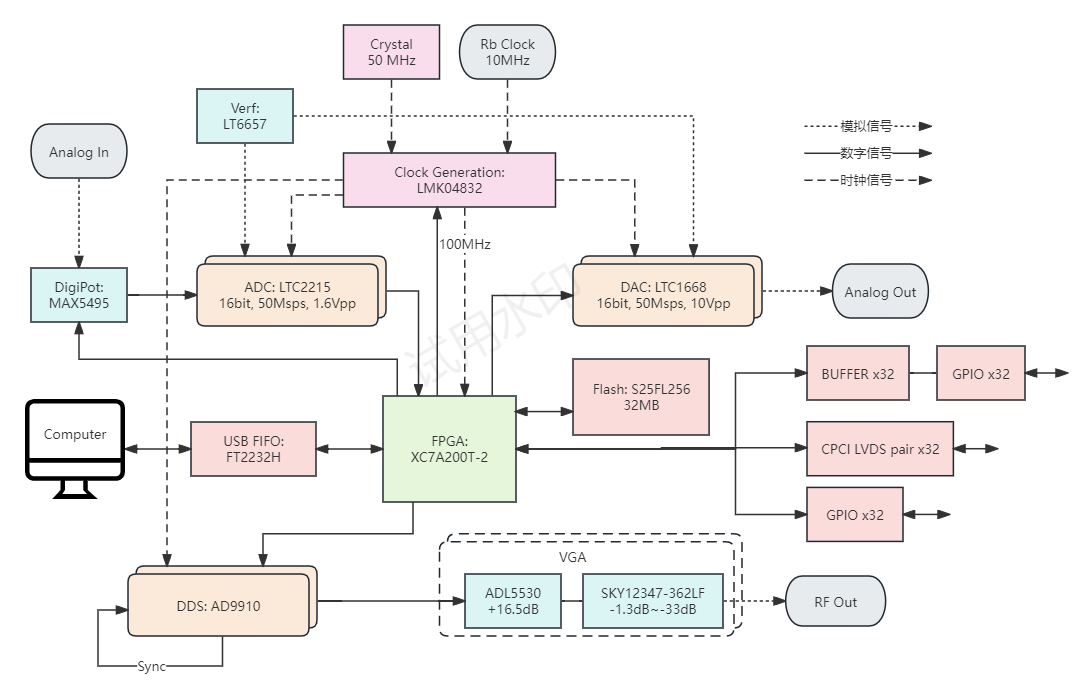
\includegraphics[width=1.0\linewidth]{rtmq/rtmq_board_structure}
\end{figure}



RTMQ测控板实物图如图\ref{fig:rtmq_board_hardware}所示,基于此硬件可以开发和部署RTMQ测控系统核心固件,此外还需要结合相应的汇编指令集(第\ref{section:fpga_rtmq}章第\ref{section:rtmq_instructions}节)来完成对系统的管理和控制\cite[]{junhua03}。当涉及到大规模拓展应用则还需要节点实时通信的链路系统(第\ref{section:fpga_rtmq}章第\ref{section:rtmq_links}节)来完成节点内部和外部通信的同步\cite[]{junhua02}。


\begin{figure}
    \centering
    \caption[RTMQ测控板去壳单板实物图]{RTMQ测控板去壳单板实物图\label{fig:rtmq_board_hardware}}
    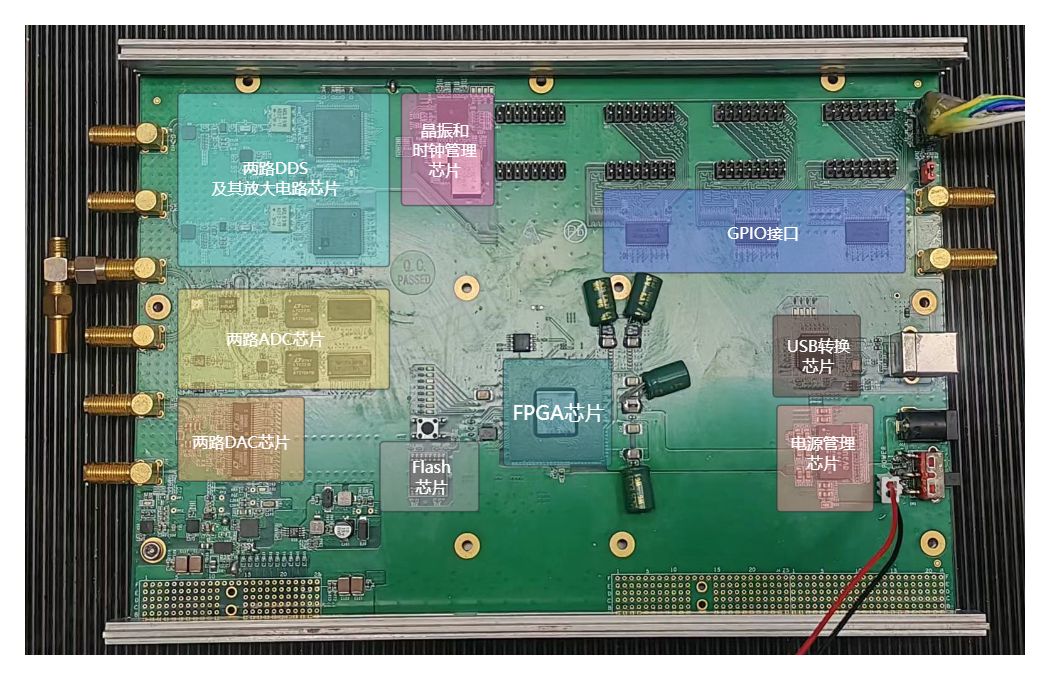
\includegraphics[width=1.0\linewidth]{rtmq/rtmq_board_hardware}
\end{figure}

\newpage
\subsection[RTMQ的重要外设拓展及其FPGA实现]{RTMQ的重要外设拓展及其FPGA实现}
% ============================================================================
% ============================================================================
% =======================   RTMQ Peripheral    ===============================
% ============================================================================
% ============================================================================

有了测控板硬件再结合RTMQ的核心固件就构成了一个可用的RTMQ测控系统板卡,而RTMQ量子测控系统的整体构成不仅需要一个专为实时可拓展量子计算设计的微处理器核心,还需要其它功能性模块的参与。因此与RTMQ架构相配套的功能性模块的固件设计开发必不可少,其中比较重要的有RTMQ通用寄存器模块、用于节点之间及与上位机通信的UART或SPI等通信模块、用于外部芯片的管理模块等,这些模块的设计和基于FPGA的固件实现将在本节接下来的内容中进行介绍。所有FPGA固件电路设计编程使用的皆是Verilog硬件描述语言,其功能仿真、综合优化及后仿真、实现、布线后仿真、板级仿真、调试与下载等都基于Xilinx公司的Vivado软件平台。

\subsubsection[RTMQ通用寄存器模块及其FPGA实现]{RTMQ通用寄存器模块及其FPGA实现}
% =======================     通用寄存器模块    ===============================
通用寄存器(General-Purpose Registers)是微处理器的一个重要功能外设,用于存储和操作微处理器中的数据。它可以用于临时存储指令和数据,以支持计算、逻辑操作和数据传输等操作,是微处理器与其它功能性外设联系的纽带。RTMQ核心的算数和逻辑运算操作、内部数据的传递和结果的储存、地址计算等都需要借助通用寄存器来实现。除此之外,通用寄存器也可以提供接口给其它功能性外设对其进行参数传递和读取,提高参数传递的速度和灵活性。接下来将介绍RTMQ系统中的通用寄存器模块及其FPGA实现结果。

通用寄存器的功能是根据微处理器请求的寄存器地址对相应的寄存器进行高速的读或写操作。如图\ref{fig:rtmq_universal_register_structure}所示,RTMQ中的通用寄存器接收来自算术逻辑单元的结果alu\_out,给出寄存器的数据输出reg\_out和副作用触发信号f\_trg。RTMQ\_AcsFlg模块的功能是根据alu\_out中寄存器地址位的值给出对该地址的寄存器的读写信号,这些信号可以是读信号(f\_read)、A指令型写信号(f\_wrt\_alu)、I指令型写高段信号(f\_wrt\_ihi)、I指令型写低段信号(f\_wrt\_ilo)。
其中alu\_out的输出结构alu\_out为:\{alu\_res, alu\_msk, alu\_rda, alu\_r0a, alu\_r1a, imm\_res, imm\_rda, imm\_seg\},其中alu\_rda为A类指令操作的目标寄存器地址、alu\_r0a和alu\_r1a为A类指令操作的两个操作寄存器地址、alu\_res和alu\_msk分别为A类指令给出的模块运算结果和结果的掩码、imm\_rda和imm\_seg分别为I类指令操作的目标寄存器地址和操作寄存器段、imm\_res为I类指令操作的模块运算结果。
% 信号具体含义如第\ref{section:rtmq_core_alu}节所述;
reg\_out是寄存器的数据输出,它的具体数据内容由reg\_out选择逻辑选择性输出;f\_trg是寄存器的副作用触发信号,当进行完A指令型写或者I指令低段写后有效,可以用来为寄存器的特定应用定义一些额外的功能。
RTMQ通用寄存器模块在Vivado中的FPGA实现结果如图\ref{fig:rtmq_universal_register}所示,其具体的接口定义如表\ref{tb:rtmq_universal_register}所示。

\begin{table}
    \centering
    \caption[RTMQ功能外设通用寄存器模块端口定义]{RTMQ功能外设通用寄存器模块端口定义\label{tb:rtmq_universal_register}}    
    \begin{tabular}{L{2.5cm}L{4cm}|L{2.5cm}L{4cm}}
        \toprule
        \multicolumn{2}{c|}{Input} & \multicolumn{2}{c}{Output} \\
        \midrule
        Port & Define & Port & Define\\
        \hline
        alu\_out[128:0] & 算术逻辑单元结果  & f\_trg & 副作用触发信号 \\
        clk             & 系统时钟          & reg\_out[31:0] & 寄存器数据输出 \\
        \bottomrule
    \end{tabular}
\end{table}

\begin{figure}
    \centering
    \caption[RTMQ用寄存器模块的设计结构图]{RTMQ用寄存器模块的设计结构图\label{fig:rtmq_universal_register_structure}}
    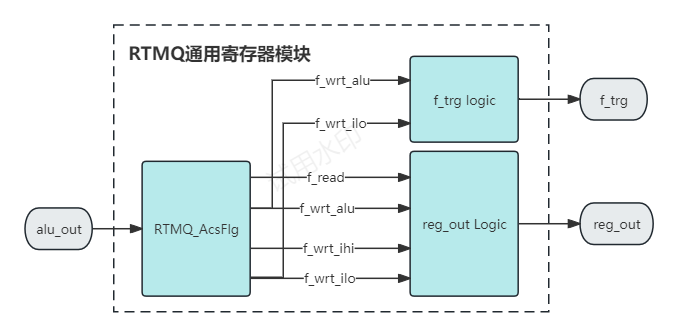
\includegraphics[width=0.7\linewidth]{rtmq/rtmq_universal_register_structure}
\end{figure}

\begin{figure}
    \centering
    \caption[RTMQ通用寄存器模块的FPGA实现结构图]{RTMQ通用寄存器模块的FPGA实现结构图(Vivado)\label{fig:rtmq_universal_register}}
    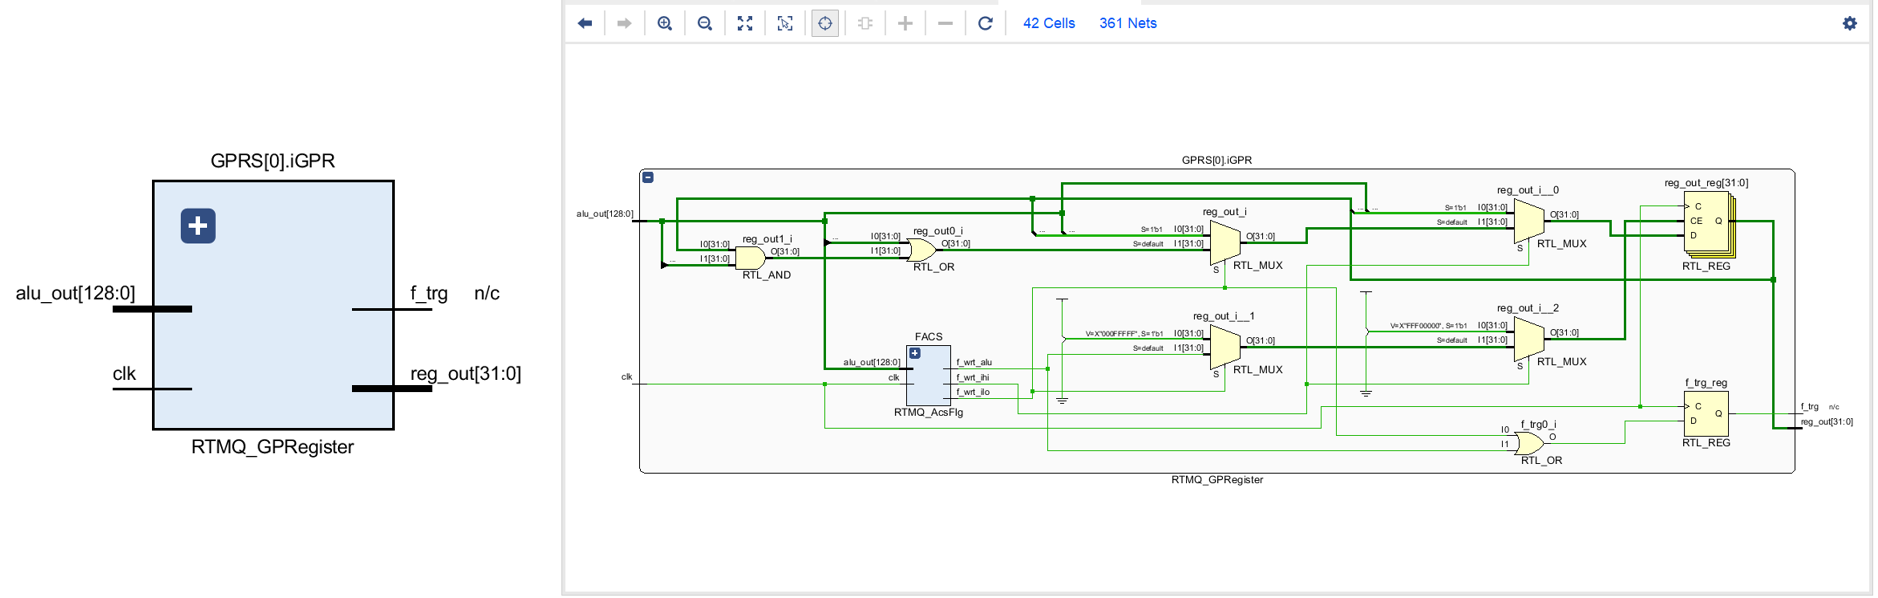
\includegraphics[width=1.0\linewidth]{rtmq/rtmq_universal_register}
\end{figure}



\subsubsection[UART模块及其FPGA实现]{UART模块及其FPGA实现}
% =======================       UART模块       ===============================
通信模块是RTMQ系统与上位机以及RTMQ系统节点之间相互传递信息的重要模块,其中UART通信模块在整个RTMQ系统中有着十分广泛的应用。UART模块即通用异步收发器(Universal Asynchronous Receiver/Transmitter),是一种串行、异步、全双工的通信协议,特点是通信线路简单,适用于远距离通信,但传输速度慢。因此该种通信方式主要应用于RTMQ系统节点与上位之间的通信以及RTMQ节点之间信息的传递。下面介绍RTMQ系统中的UART模块及其FPGA实现结果。

% \begin{table}
%     \centering
%     \caption[UART数据通信格式]{UART数据通信格式。起始位之前和停止位之后是空闲位;最低位LSB到最高位MSB之间为有效数据位;奇偶校验位在MSB之后。\label{tb:rtmq_uart_data}}    
%     \begin{tabular}{C{0.9cm}|C{0.85cm}C{0.4cm}C{0.4cm}C{0.4cm}C{0.4cm}C{0.4cm}C{0.4cm}C{0.4cm}C{0.4cm}C{0.85cm}|C{0.9cm}C{0.9cm}|C{0.9cm}}
%         \toprule
%         &\multicolumn{12}{c}{第n个字节数据流}& \\
%         \midrule
%         1 & 0 & X & X & X & X & X & X & X & X & X & X & 1 & 1 \\
%         \hline
%         空闲位 & 起始位 & LSB & & & & & & & & MSB & 奇偶校验位 & 停止位 & 空闲位 \\ 
%         \bottomrule
%     \end{tabular}
% \end{table}

% UART是一种串行、异步、全双工的通信协议,它的数据通信格式如表\ref{tb:rtmq_uart_data}所示。根据UART协议,初始时总线处于空闲状态,即信号线为高电平“1”(空闲位);每次传输开始时对方先发出一个低电平“0”(起始位);起始位之后就是数据位,可以是6、7、8、9位等等,先发送低位再发送高位,使用低电平表示‘0’高电平表示‘0’(有效数据位);根据事先规定,数据位加上这一位后,使得“1”的位数应为偶数(偶校验)或奇数(奇校验),以此来校验数据传送的正确性(奇偶校验位);一次字符数据传输结束后给出若干位高电平指示本字节传输结束,可以是1位、1.5位、2位等(停止位)。

UART模块的设计结构如图\ref{fig:rtmq_uart_structure}所示,模块的组成主要有RTMQ通用寄存器模块、UART发送模块、UART接收模块和数据处理模块部分。
该模块的输入为RTMQ算术逻辑单元输入alu\_out、UART接收输入uart\_rx,输出为配置指令输出cfg\_ins、配置指令覆盖标志f\_cfg、UART发送信号uart\_rx、发送结束标志f\_tx\_done等。需要发送数据时,算术逻辑单元输入alu\_out向通用寄存器写入数据,随后通用寄存器给出数据d\_txd和副作用触发信号f\_snd到UART模块中进行传输,UART发送模块使用uart\_tx按协议传输数据,结束时给出f\_tx\_done指示信号;需要接收数据时,来自对方发送模块的数据传入UART接收模块,接收模块按协议接收信息并通过dat\_rx传输到数据处理模块中逐个保存,传输结束后给出f\_fin指示信号,数据处理模块将收到数据的最高位作为f\_cfg指示信号输出,其余为作为cfg\_ins配置指令输出。
UART通信模块在Vivado中的FPGA实现结果如图\ref{fig:rtmq_uart}所示,其具体的接口定义如表\ref{tb:rtmq_uart}所示。


\begin{figure}
    \centering
    \caption[RTMQ功能外设UART模块的设计结构图]{RTMQ功能外设UART模块的设计结构图\label{fig:rtmq_uart_structure}}
    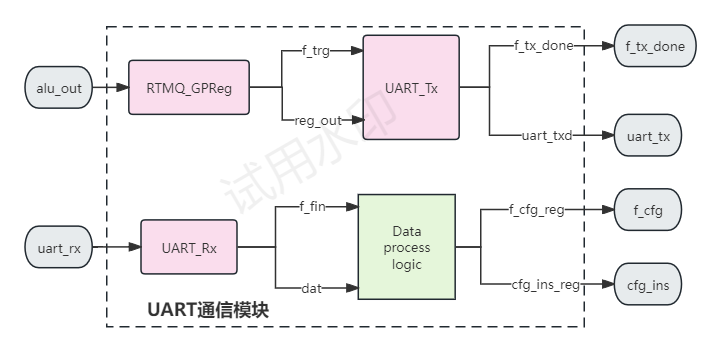
\includegraphics[width=0.8\linewidth]{rtmq/rtmq_uart_structure}
\end{figure}

\begin{table}
    \centering
    \caption[RTMQ功能外设UART模块端口定义]{RTMQ功能外设UART模块端口定义\label{tb:rtmq_uart}}    
    \begin{tabular}{L{2.5cm}L{4cm}|L{2.5cm}L{4cm}}
        \toprule
        \multicolumn{2}{c|}{Input} & \multicolumn{2}{c}{Output} \\
        \midrule
        Port & Define & Port & Define\\
        \hline
        alu\_out[128:0] & 算术逻辑单元结果  & cfg\_ins[31:0] & 模块配置指令 \\
        clk             & 系统时钟          & f\_cfg & 配置指令覆盖标志 \\
        uart\_rx        & UART接受信号Rx    & f\_tx\_done & 发送信号结束标志 \\
        &               & uart\_tx          & UART发送信号Tx\\
        \bottomrule
    \end{tabular}
\end{table}

\begin{figure}
    \centering
    \caption[RTMQ功能外设UART模块的FPGA实现结构图]{RTMQ功能外设UART模块的FPGA实现结构图(Vivado)\label{fig:rtmq_uart}}
    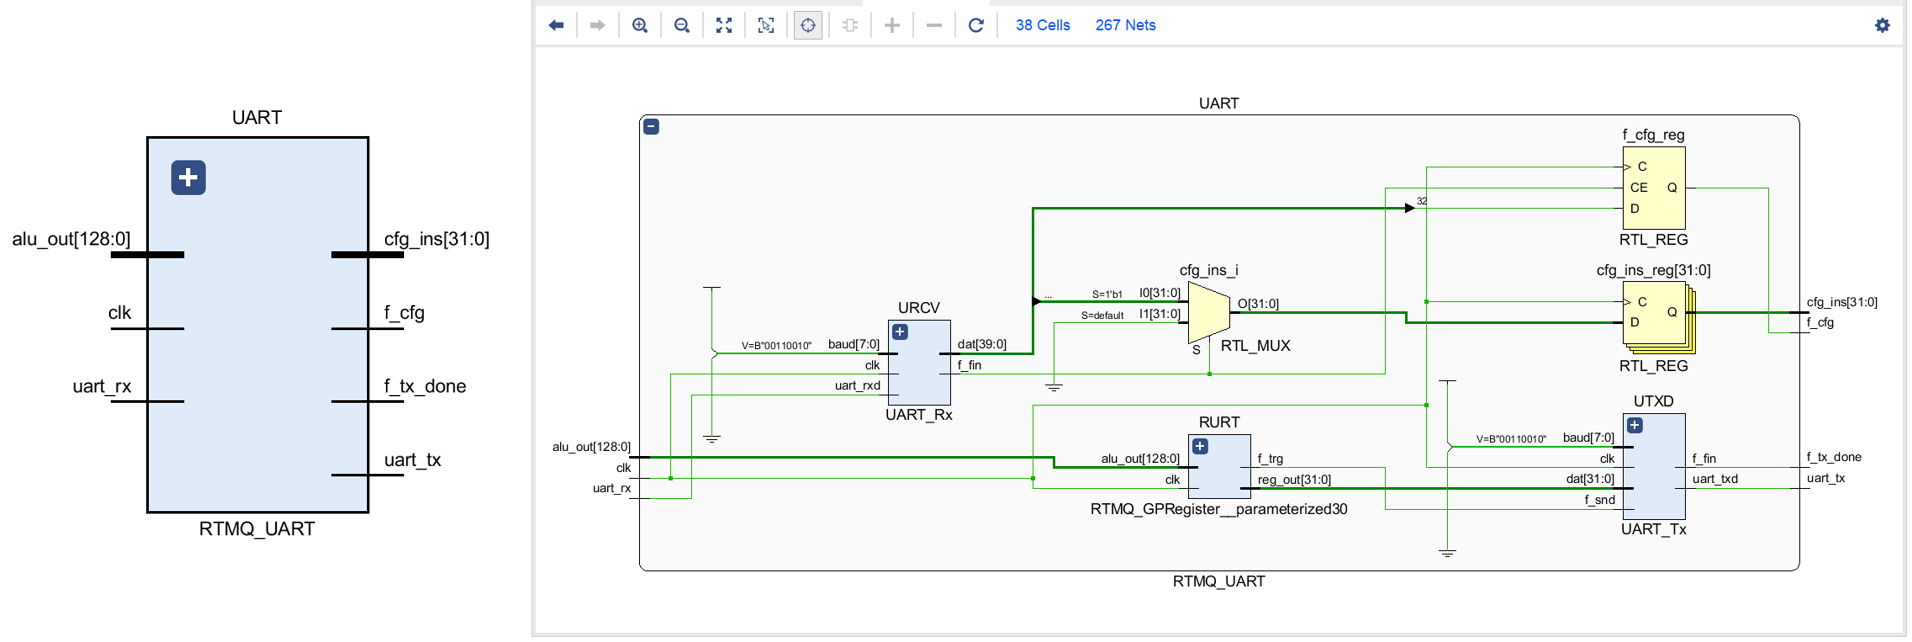
\includegraphics[width=1.0\linewidth]{rtmq/rtmq_uart}
\end{figure}




\subsubsection[SPIMaster模块及其FPGA实现]{SPIMaster模块及其FPGA实现}
% =======================        SPI模块       ===============================

RTMQ系统中不仅涉及与上位机和不同RTMQ节点间相互的通信,还需要与一些如板上的其它功能芯片进行高速通信。在高速通信的场景下UART通信协议的应用很受限,因此需要一种可以支持高速通信的协议来满足需求——SPI(串行外围设备接口,Serial Perripheral Interface)。SPI是一种高速、全双工、同步的通信总线,它常用于EEPROM、Flash、实时时钟(RTC)、数模转换器(ADC)、数字信号处理器(DSP) 以及数字信号解码器之间。RTMQ系统的微处理器即采用SPI进行外部功能拓展设备的管理,如与板上集成的AD9910芯片间的通信等,因此这里主要介绍SPIMaster模块的实现。

\begin{figure}
    \centering
    \caption[SPI主从设备连接图]{SPI主从设备连接图。\label{fig:rtmq_spi_connection1}}
    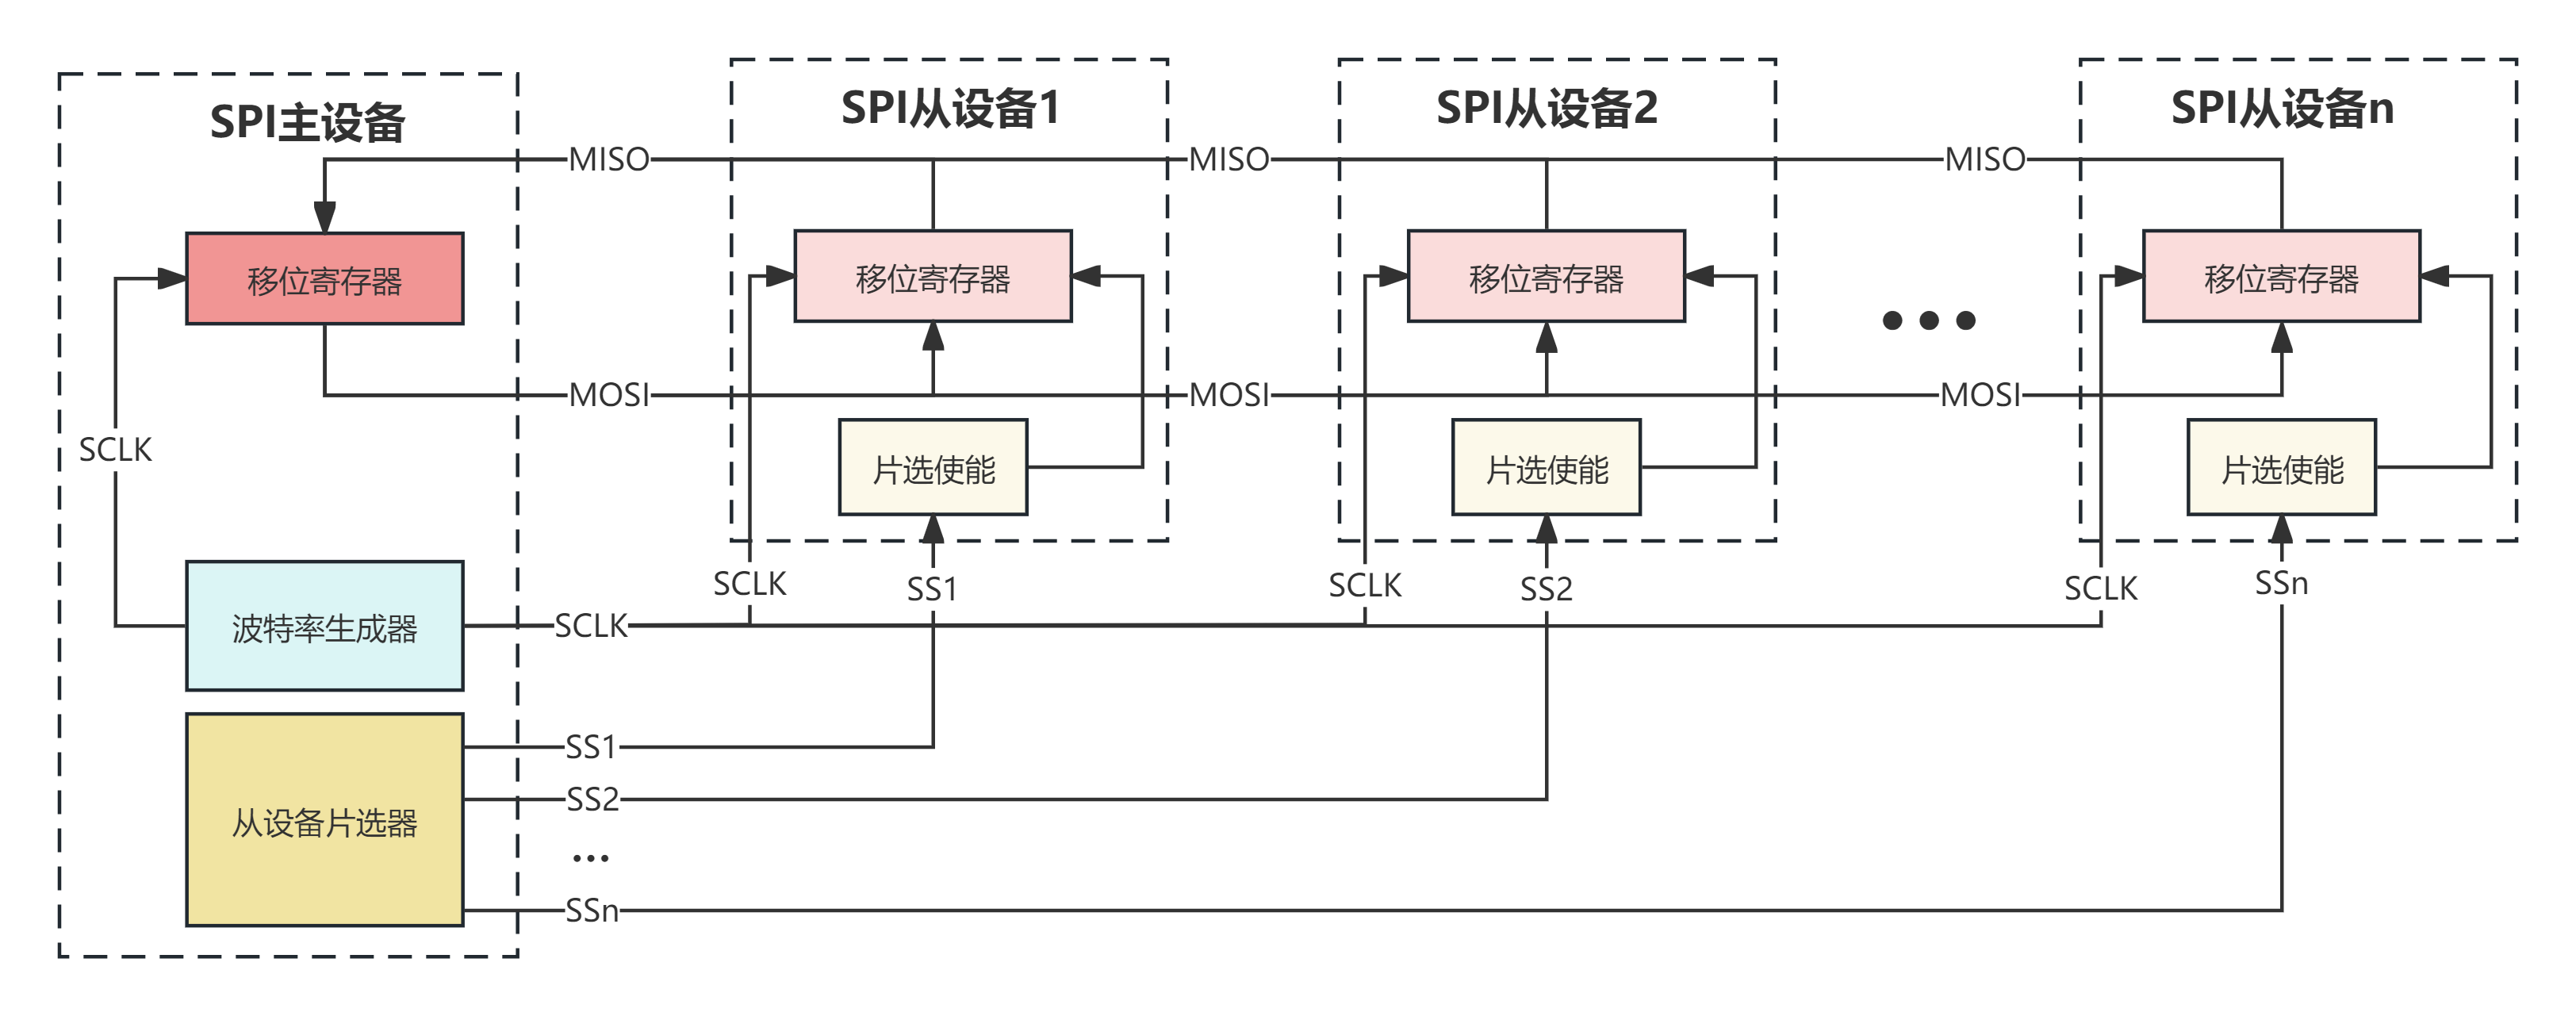
\includegraphics[width=1.0\linewidth]{rtmq/rtmq_spi_connection1}
\end{figure}

SPI是一种主从通信协议,只有一个主设备通过片选选择不同的从设备。主设备和多个从设备的连接如图\ref{fig:rtmq_spi_connection1}所示,每一个传输周期内SPI主设备与被片选到的SPI从设备(SSn)通过移位寄存器交换数据,在此过程中的通信时钟SCLK统一由SPI主设备产生并分发给各个SPI从设备。根据时钟空闲时的电平高低和采样发生在上升沿还是下降沿SPI可以有四种通信模式,几种模式之间没有本质区别,但要注意主从设备进行SPI通讯时要确保它们的传输模式设置相同。
SPIMaster模块设计结构如图\ref{fig:rtmq_spi_master_structure}所示,主要涉及到的模块有输出位移寄存器、输入位移寄存器、SPIMaster核心逻辑模块等。
该模块的输入为RTMQ算术逻辑单元结果alu\_out和主收从发信号miso,输出包括控制信号reg\_sctl、SPI从模块片选地址、SPI片选信号csb、SPI传输结束标志f\_spi\_done、主发从收信号mosi、SPI主模块生成时钟sclk、SPI主模块接收到的数据reg\_sdat。
当SPIMaster需要发送数据时,使用alu\_out将要发送的内容写入输出位移寄存器中等待发送,然后将SPI的控制信号配置写入通用寄存器,写入结束后通用寄存器会给出副作用触发信号传递给SPIMaster核心模块的发送使能端口f\_snd,同时输出位移寄存器将要发送的内容传递给ins\_buf逻辑模块,该模块将要发送的数据内容和来自reg\_sctl的要发送的目标地址dst\_adr整合后传递给SPIMaster的核心模块发送,SPIMaster核心模块内部将要发送的数据按照SPI通信方式与被csb信号片选到的SPI从机使用sclk时钟通过mosi线路进行通信;当SPIMaster要读取数据是时,过程与发送数据时类似,不过通信过程完成后来自从机的有用数据将被保存在输出位移寄存器模块中并用f\_spi\_done指示有效,可被RTMQ微处理器访问获取。控制信号reg\_sctl还包含SPI主收从发信号的时延配置信号miso\_ltn、比特数bit\_cnt以及时钟分频等信号用于对SPIMaster核心模块进行配置;SPIMaster核心模块的cpha和cpol用以配置SPI的工作模式,一般使用宏进行全局统一定义。SPIMaster通信模块在Vivado中的FPGA实现如图\ref{fig:rtmq_spi}所示,其具体的接口定义如表\ref{tb:rtmq_spi}所示。



\begin{figure}
    \centering
    \caption[SPIMaster模块设计结构图]{SPIMaster模块设计结构图\label{fig:rtmq_spi_master_structure}}
    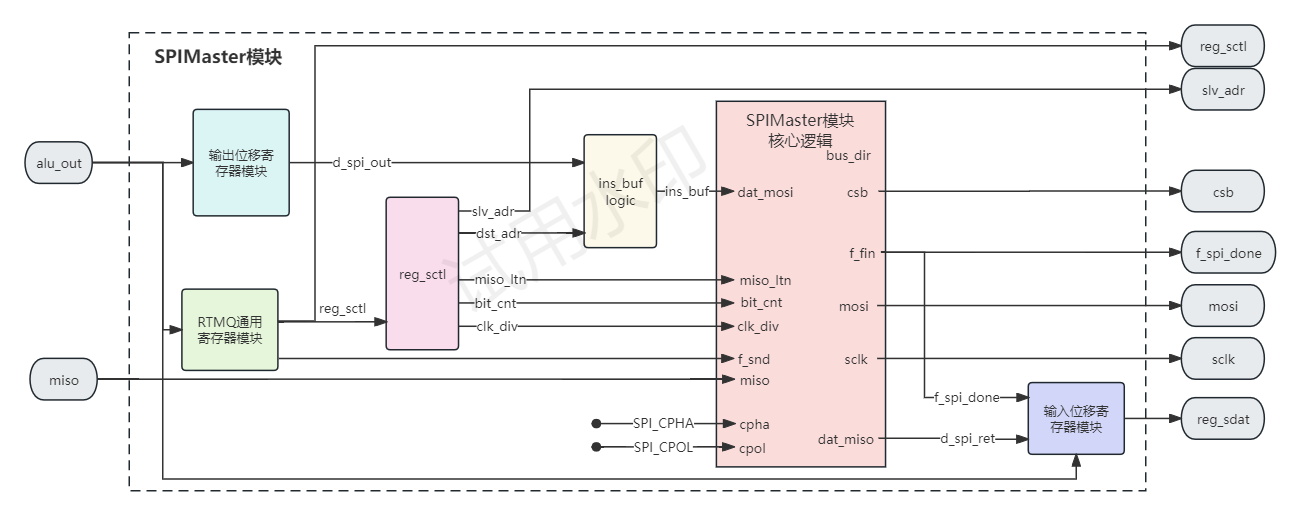
\includegraphics[width=1.0\linewidth]{rtmq/rtmq_spi_master_structure}
\end{figure}


\begin{table}
    \centering
    \caption[RTMQ功能外设SPIMaster模块端口定义]{RTMQ功能外设SPIMaster模块端口定义\label{tb:rtmq_spi}}    
    \begin{tabular}{L{2.5cm}L{4cm}|L{2.5cm}L{4cm}}
        \toprule
        \multicolumn{2}{c|}{Input} & \multicolumn{2}{c}{Output} \\
        \midrule
        Port & Define & Port & Define\\
        \hline
        alu\_out[128:0] & 算术逻辑单元结果 & csb &  \\
        clk & 系统时钟 & f\_spi\_done & SPI Rx/Tx结束标志 \\
        miso & 主收从发信号 & mosi & 主发从收信号 \\
        & & reg\_sctl[31:0] & \\
        & & reg\_sdat[31:0] & \\
        & & sclk & 主设备产生的时钟信号 \\
        & & slv\_adr[2:0] & 目标从设备地址\\

        \bottomrule
    \end{tabular}
\end{table}

\begin{figure}
    \centering
    \caption[RTMQ功能外设SPIMaster模块的实现结构图]{RTMQ功能外设SPIMaster模块的实现结构图(Vivado)\label{fig:rtmq_spi}}
    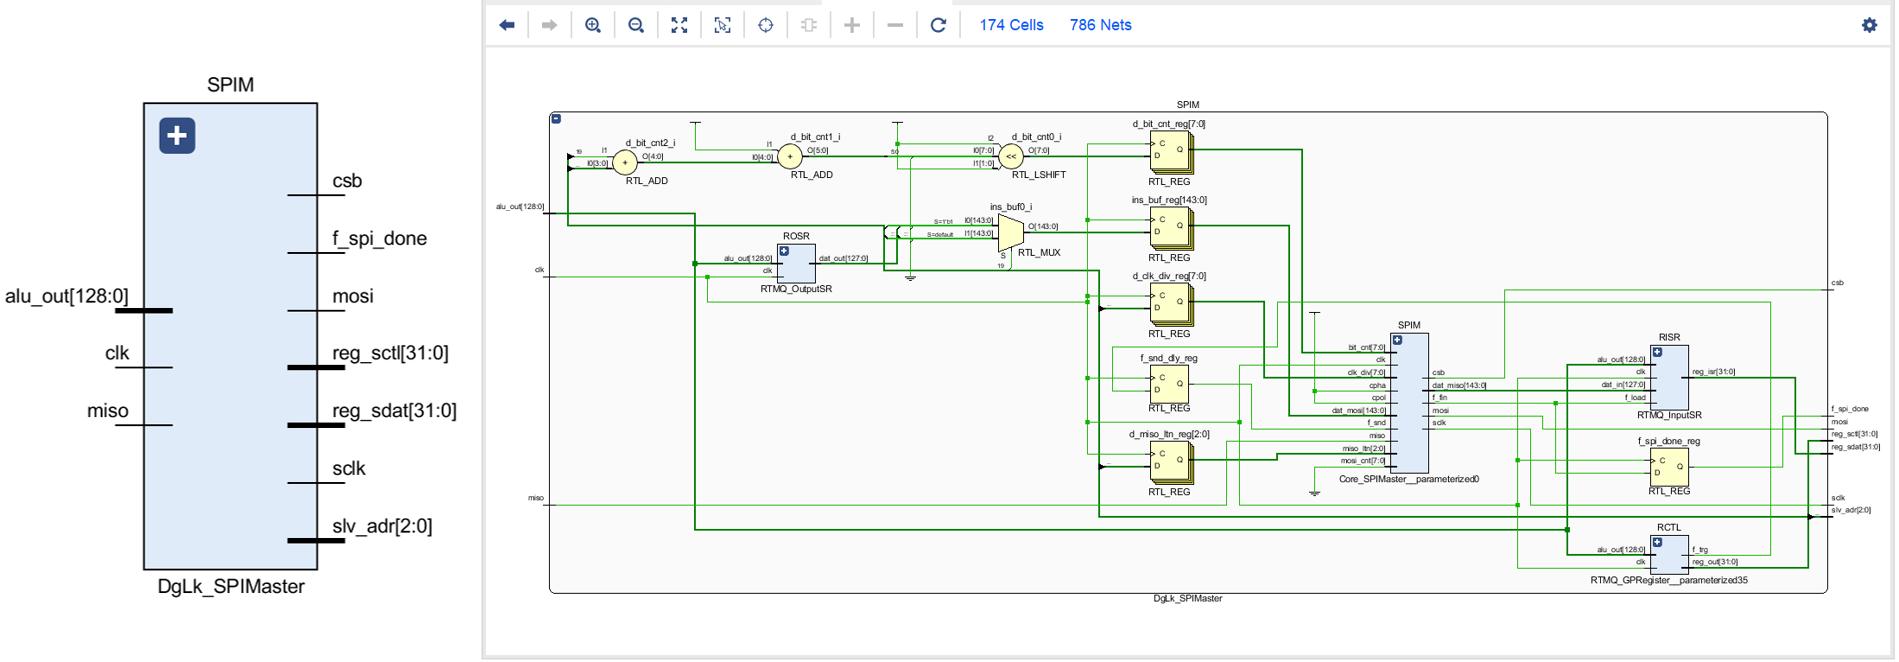
\includegraphics[width=1.0\linewidth]{rtmq/rtmq_spi}
\end{figure}



\subsubsection[AD9910芯片管理模块及其FPGA实现]{AD9910芯片管理模块及其FPGA实现}
% =======================    AD9910管理模块     ===============================



AD9910芯片是一个多功能的DDS芯片,它不仅可以通过寄存器配置射频输出幅度、频率、相位等参数,还可以提前设置多种预定义的参数策略在使用时通过外部选择信号进行灵活切换。除此之外,它还可以配置为并行输入模式对幅度、频率或相位进行高速调制。而AD9910芯片的各项功能配置需要依赖SPI串口对其内部的配置寄存器进行配置,于是AD9910芯片管理模块应运而生。

\begin{figure}
    \centering
    \caption[AD9910芯片管理模块设计结构图]{AD9910芯片管理模块设计结构图\label{fig:rtmq_ad9910_structure}}
    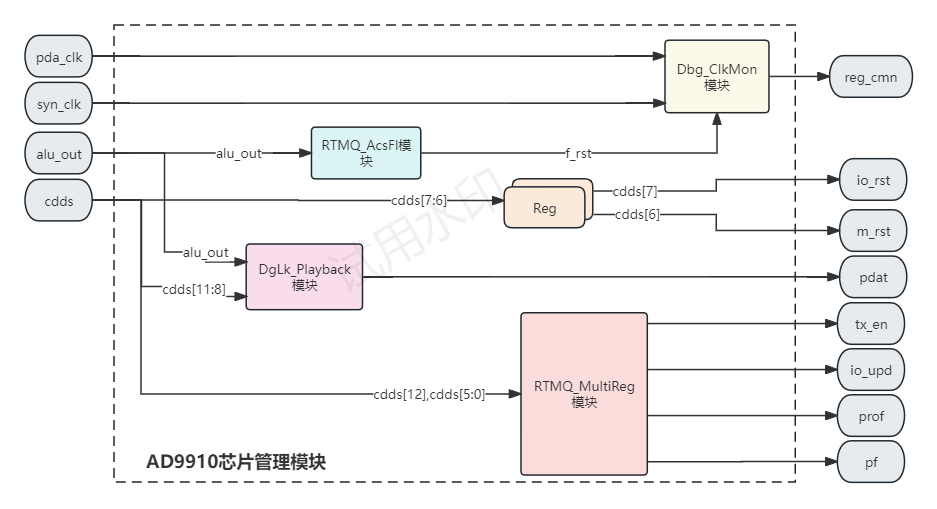
\includegraphics[width=0.8\linewidth]{rtmq/rtmq_ad9910_structure}
\end{figure}


\begin{table}
    \centering
    \caption[AD9910芯片管理模块端口定义]{AD9910芯片管理模块端口定义\label{tb:rtmq_ad9910}}    
    \begin{tabular}{L{2.5cm}L{4cm}|L{2.5cm}L{4cm}}
        \toprule
        \multicolumn{2}{c|}{Input} & \multicolumn{2}{c}{Output} \\
        \midrule
        Port & Define & Port & Define\\
        \hline
        alu\_out[128:0] & 算术逻辑单元结果  & io\_rst & 输入输出重置信号 \\
        cdds[8:0]      & DDS控制信号       & io\_upd & 输入输出更新信号 \\
        clk             & 系统时钟          & m\_rst & 主机重置信号 \\
        pda\_clk        & PD时钟            & pdat[15:0] & 并行数据 \\
        syn\_clk        & 同步时钟          & pf[1:0] & 并行数据目标 \\
        p\_dat[15:0]    & 并行数据       & prof & 配置策略选择\\
                        &                   & reg\_cmn[31:0] & 时钟相位检测\\
                        &                   & tx\_en & 发送使能信号\\
        \bottomrule
    \end{tabular}
\end{table}


\begin{figure}
    \centering
    \caption[AD9910芯片管理模块的实现结构图]{AD9910芯片管理模块的实现结构图(Vivado)\label{fig:rtmq_ad9910}}
    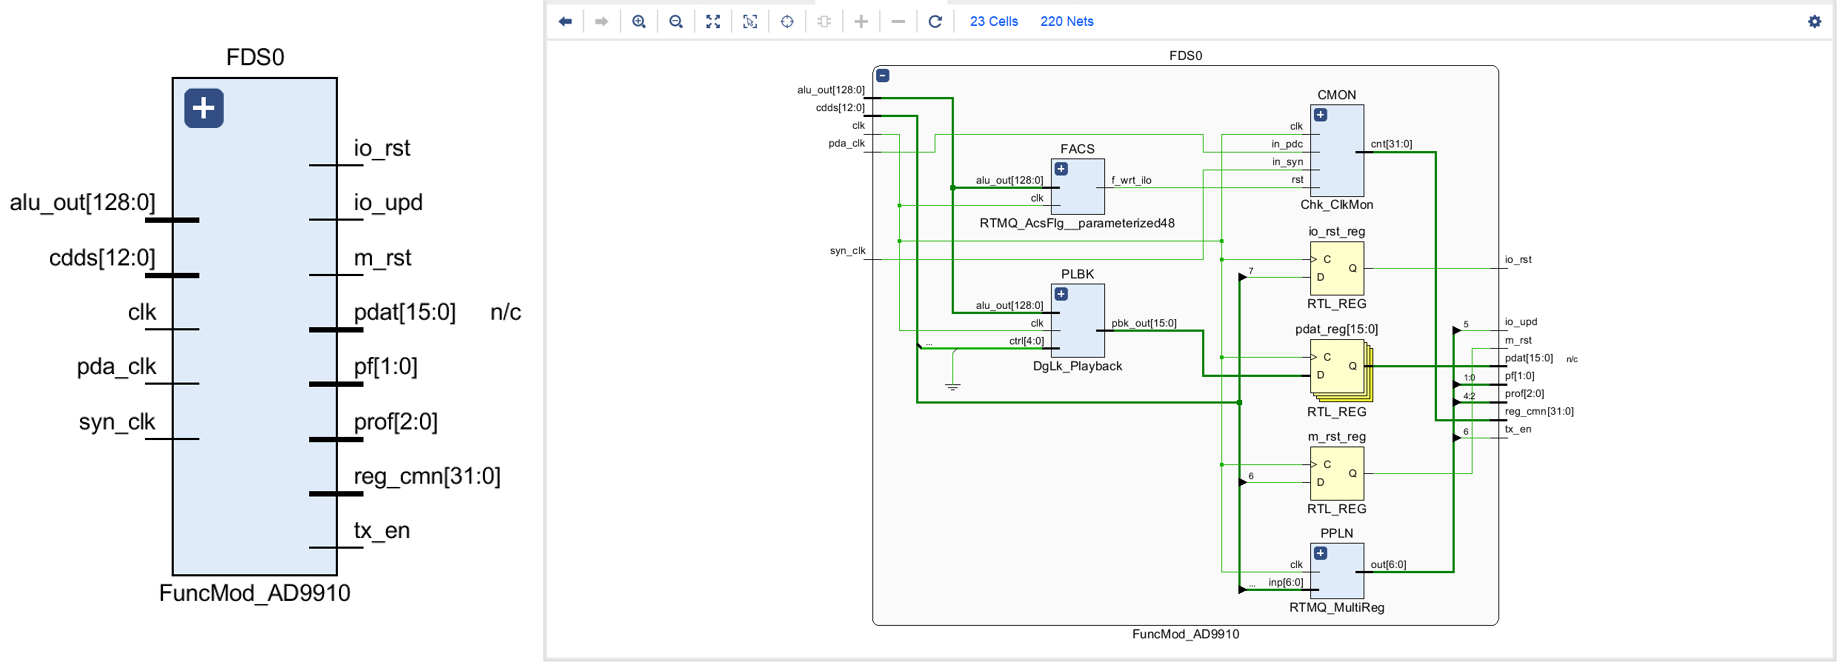
\includegraphics[width=1.0\linewidth]{rtmq/rtmq_ad9910}
\end{figure}

AD9910芯片管理模块设计结构如图\ref{fig:rtmq_ad9910_structure}所示,它的输入有算术逻辑单元结果alu\_out、PD时钟pda\_clk、同步时钟syn\_clk、并行数据输入p\_dat,DDS控制信号cdds,输出包括时钟相位检测reg\_cmn、输入输出重置信号io\_rst、主机重置信号m\_rst、并行数据pdat、发送使能信号tx\_en、输入输出更新信号io\_upd、配置策略选择prof、并行数据目标pf。其中RTMQ\_AcsFI模块和Chk\_ClkMon模块接收PD时钟pda\_clk和同步时钟syn\_clk进行对比输出时钟相位检测结果reg\_cmn用来对两时钟进行检查。cdds是一个9位的控制信号,其中第6、7位分别用来控制主机重置和输入输出重置;cdds的第0到5位和第12位这几个信号经过RTMQ\_MultiReg进行一定的时延(约为10个时钟周期,以平滑DDS芯片各模式之间的切换)对应输出信号,
第0到1位对应pf信号,第2到4位对应prof信号,第5位对应io\_upd,第12位对应tx\_en信号。输入的p\_dat,也即输出的pdat是向AD9910芯片输出的并行数据,该信号用作DDS并行调制模式的输入。AD9910芯片管理模块在Vivado中的FPGA实现如图\ref{fig:rtmq_ad9910}所示,其具体的接口定义如表\ref{tb:rtmq_ad9910}所示。


\subsubsection[ADC芯片管理模块及其FPGA实现]{ADC芯片管理模块及其FPGA实现}
% =======================      ADC管理模块      ===============================

ADC芯片管理模块只需要将来自ADC的数据进行缓存和寄存使之可以让RTMQ微处理器按照想要的时钟来稳定地获取到有效数据即可。ADC芯片管理模块的输入为ADC芯片的数据输出,该模块的功能为根据实际需求对ADC芯片的数据进行采样输出,当不进行采样时该模块的输出保持不变。

如图\ref{fig:rtmq_adc_structure}所示,来自ADC芯片的数据adc\_in作为模块输入,为了匹配ADC芯片的刷新速率与实际需求采样时钟速率,模块内部将ADC的数据进行缓存得到adc\_buf并对时钟输入adc\_smp使用边沿检测获得信号e\_smp,随后对其进行一定的时延来控制最终的有效ADC数据输出reg\_aio。
ADC芯片管理模块在Vivado中的FPGA实现如图\ref{fig:rtmq_adc}所示,其具体的接口定义如表\ref{tb:rtmq_adc}所示。
% \textcolor{green}{具体内容描述待补充。}

\begin{figure}
    \centering
    \caption[ADC芯片管理模块的设计结构图]{ADC芯片管理模块的设计结构图。\label{fig:rtmq_adc_structure}}
    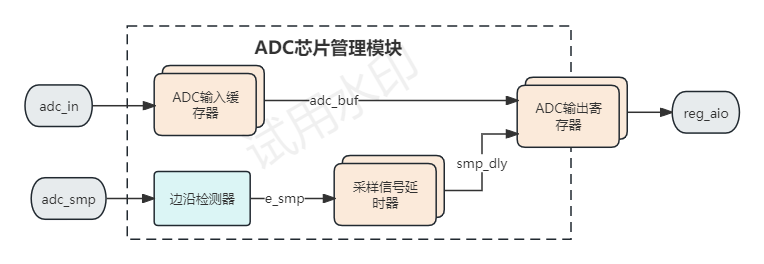
\includegraphics[width=0.7\linewidth]{rtmq/rtmq_adc_structure}
\end{figure}


\begin{table}
    \centering
    \caption[RTMQ系统外设AD9910芯片管理模块端口定义]{RTMQ系统外设AD9910芯片管理模块端口定义\label{tb:rtmq_adc}}    
    \begin{tabular}{L{2.5cm}L{4cm}|L{2.5cm}L{4cm}}
        \toprule
        \multicolumn{2}{c|}{Input} & \multicolumn{2}{c}{Output} \\
        \midrule
        Port & Define & Port & Define\\
        \hline
        adc\_in[15:0]   & ADC采样数据   & reg\_aio[15:0] & ADC输出数据 \\
        adc\_smp        & ADC采样时钟   &  &  \\
        clk             & 系统时钟      &  &  \\
        \bottomrule
    \end{tabular}
\end{table}




\begin{figure}
    \centering
    \caption[ADC芯片管理模块的FPGA实现结构图]{ADC芯片管理模块的FPGA实现结构图(Vivado)\label{fig:rtmq_adc}}
    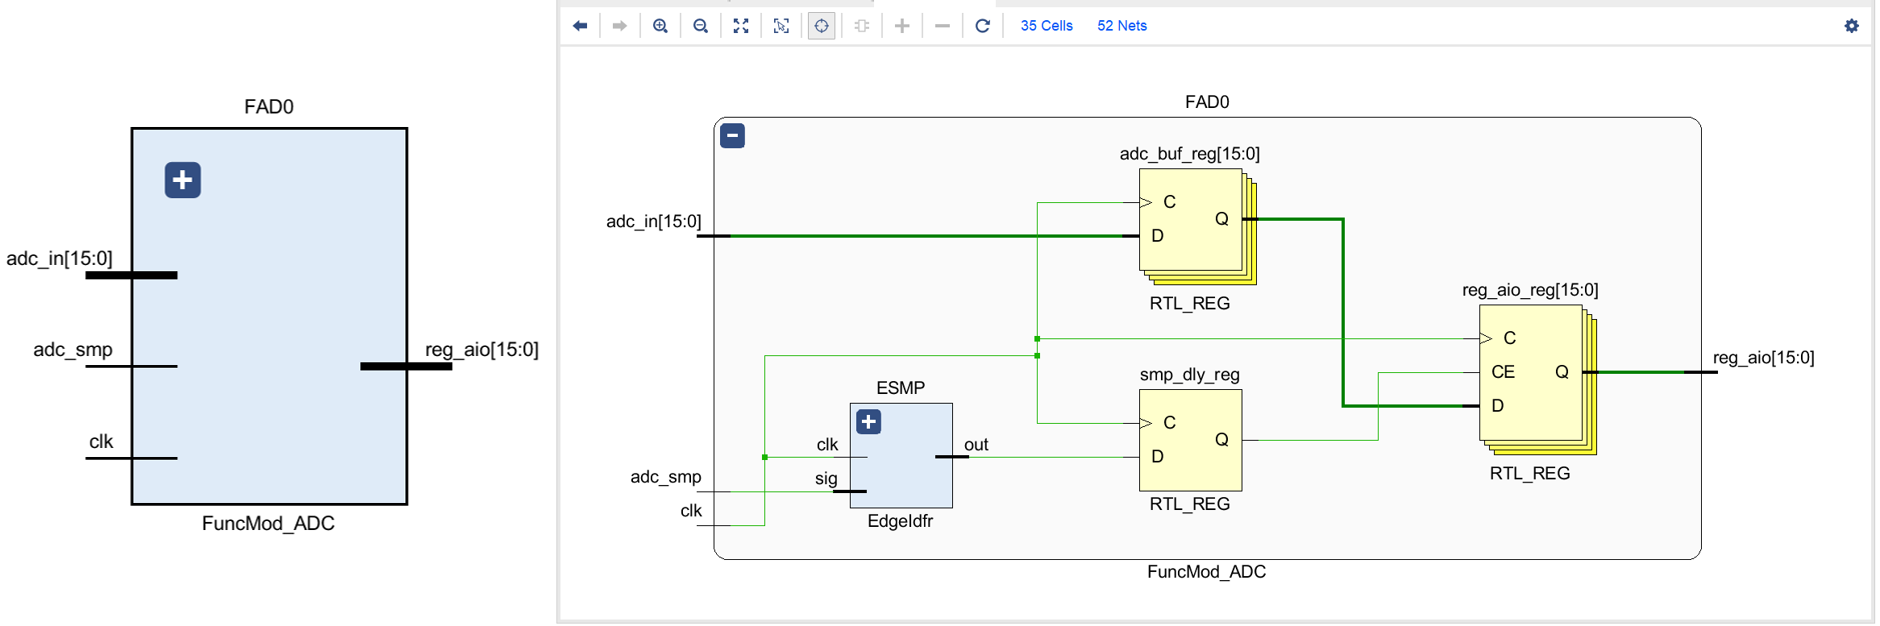
\includegraphics[width=1.0\linewidth]{rtmq/rtmq_adc}
\end{figure}






\newpage
\section[基于RTMQ的离子阱频率稳定]{基于RTMQ的离子阱频率稳定\label{section:trap_frequency_stablization}}
% ============================================================================
% ============================================================================
% =======================     离子阱频率稳定    ===============================
% ============================================================================
% ============================================================================

在前述的基本理论理解及RTMQ测控系统的软硬件基础上,可以结合具体的实验需求实现离子量子计算的一些重要子系统的构建以至于整个量子计算系统的建立。
如第\ref{section:quantum_computation}章第\ref{section:ion_trap_motion}节中讨论的,带电粒子通常由射频(RF)电势控制,其场梯度提供时间平均力,这些力构成了四极质量滤波器、离子质谱仪和射频(Paul)离子阱等应用的基础\cite[]{Dehmelt_1990, Paul_1990}。这些射频电势,通常在 1 kHz 到 100 MHz 的频率处数百或数千个伏特,在真空中驱动高阻抗负载,通常由射频放大器和谐振升压变换器(例如四分之一波或螺旋谐振器)产生\cite[]{Siverns_Simkins_Weidt_Hensinger_2012}。这种电路容易受到放大器增益、变压器的机械振动和系统中的温度漂移的波动的影响。离子阱对这些波动特别敏感,因为射频电势决定了被捕获离子的谐波振荡频率。稳定的阱频率在从量子信息处理\cite[]{Blatt_Wineland_2008, Monroe_Kim_2013}和量子模拟\cite[]{Richerme_Gong_Lee_Senko_Smith_Foss_Feig_Michalakis_Gorshkov_Monroe_2014, Jurcevic_Lanyon_Hauke_Hempel_Zoller_Blatt_Roos_2014}到原子运动的量子态的制备\cite[]{Leibfried_Blatt_Monroe_Wineland_2003}、原子干涉测量\cite[]{Johnson_Neyenhuis_Mizrahi_Wong_Campos_Monroe_2015}、和量子有限计量\cite[]{Chou_Hume_Koelemeij_Wineland_Rosenband_2010}等方面至关重要。


理论上离子阱中影响阱频率的各种因素
在离子阱系统中,阱频率的表达式为:
\begin{align}
    \omega=e\mu V_0/\sqrt{2}m\Omega R^2 \label{eq:trap_frequency}
\end{align}

这些参数分别是:
\begin{itemize}
    \item $e$: 离子电荷量;
    \item $\mu$: 几何效率因子;
    \item $m$: 粒子质量;
    \item $R$: 电极间距;
    \item $\Omega$: 输入射频信号的频率;
    \item $V_0$: 输入信号的电压;
\end{itemize}


上面的各个参数中$e$,$\mu$,$m$是常数,R在阱几何形状确定的情况下也是常数。因此,关键的参数在于与射频相关的 $\Omega$ 和 $V_0$ 。这其中,当今射频生成器件自身的频率和幅度稳定性是相当高的,可能产生抖动因素的实际上主要是经过谐振腔后的输出幅度。我们使用的螺线管谐振腔$Q$值较高,只要谐振腔的中心透过频率稍微发生偏移,输出幅度就可能发生较大的抖动。因此阱频稳定主要是通过稳定谐振腔输出的射频幅度实现的。本节接下来将首先介绍一种RTMQ的重要功能外设拓展——高速通用数字PID的设计及其FPGA实现,随后介绍利用RTMQ测控系统并结合该数字PID实现离子阱频稳定系统的原理及其搭建和测试结果。

\subsection[RTMQ功能拓展高速通用数字PID及其FPGA实现]{RTMQ功能拓展高速通用数字PID及其FPGA实现\label{section:digital_pid}}
% ============================================================================
% =======================      高速数字PID      ===============================
% ============================================================================

各类参数稳定的控制系统构建常常可以使用各式各样的反馈控制器来完成,其中最方便使用最广泛的控制器为PID控制器,即比例-积分-微分控制器。当前量子计算系统中大量采用PID控制器进行诸如激光功率稳定、激光相位稳定、激光拍频稳定等控制系统的构建,常用的器件有如LB1005模拟伺服控制器。这类模拟控制器的确定在于稳定性较差且价格昂贵,此外它的集成度也比较差,往往需要占用较大的实验平台面积。除此之外这类模拟PID控制器往往采用机械旋钮进行参数调节,不利于进行实验系统的集成化和自动化。与之相比较,使用融合了高速通用数字PID的RTMQ测控系统可以同时完成对实验序列的操控和对设备关键参数的伺服控制。除此之外,采用也对系统完成了集成化和数字化,提高了系统的稳定性和易用性。
% \subsubsection[数字PID]{数字PID}
数字PID控制器是一种常用的自动控制算法,用于实现对系统的闭环控制。PID控制器通过对系统的误差进行比例(Proportional)、积分(Integral)和微分(Derivative)计算,生成控制信号来调整系统的输出,以达到期望的控制效果。在量子测控系统中很多地方都需要用到闭环控制,比如激光的功率稳定、激光的波长稳定、离子阱频率稳定等。相对于模拟PID控制器,数字PID控制器具有结构简单、易于实现、控制灵活、工作稳定等优点,是RTMQ系统中的重要功能外设拓展。

PID 控制器的数学表达式可以表示为:
\begin{align}
    u(t)= K_p e(t) + K_i \int_{0}^{t} e(\tau) d\tau + K_d \frac{d e(t)}{dt}
\end{align}

其中,$u(t)$是控制器的输出,$e(t)$是系统的误差,$K_p$、$K_i$和$K_d$分别是比例系数、积分系数和微分系数。
 
PID控制器的实现可以分为模拟PID和数字PID两种方式。模拟PID是通过模拟电路实现的,而数字PID是通过数字计算实现的。数字PID控制器通常使用微处理器或计算机来实现,其基本结构包括采样、计算和输出三个部分。数字 PID 控制器的实现步骤如下:
\begin{itemize}
    \item 采样:对系统的输入和输出进行采样,获取当前时刻的误差值e(t);
    \item 计算:根据采样得到的误差值,按照 PID 控制器的数学表达式计算控制信号u(t);
    \item 输出:将计算得到的控制信号输出到执行机构,调整系统的输出;
\end{itemize}

要想实现数字PID控制器,首先需要对其中的比例、积分和微分操作进行离散化处理。常用的离散化方法有矩形法和梯形法。矩形法将积分区间划分为若干个相等的子区间,每个子区间的积分值近似为矩形的面积;梯形法将积分区间划分为若干个相等的子区间,每个子区间的积分值近似为梯形的面积。这一步骤在嵌入式系统中通常使用模拟数字转换(ADC)芯片来完成。

\subsubsection[数字PID的增量表达式]{数字PID的增量表达式}
硬件资源在FPGA中是十分宝贵的资源,而乘法器这样的器件往往会占用大量的硬件资源。因此在满足时序要求的情况下我们希望能够尽量减少乘法器的使用,PID的增量表达式就是一种可以有效减少PID硬件电路实现过程中乘法器需求个数的方式,下面将介绍这种方法。

\begin{figure}
    \centering
    \caption[数字PID结构示意图]{数字PID结构示意图。MULT:乘法器模块;Reg:寄存器模块;ADD:加法器模块;SUB:减法器模块;LIM:限幅器模块;$y_t, u_t$:输入和输出信号;$ref$:参考值输入;$k_0, k_1, k_2$:增量表达下的PID控制参数。\label{fig:rtmq_pid_structure}}
    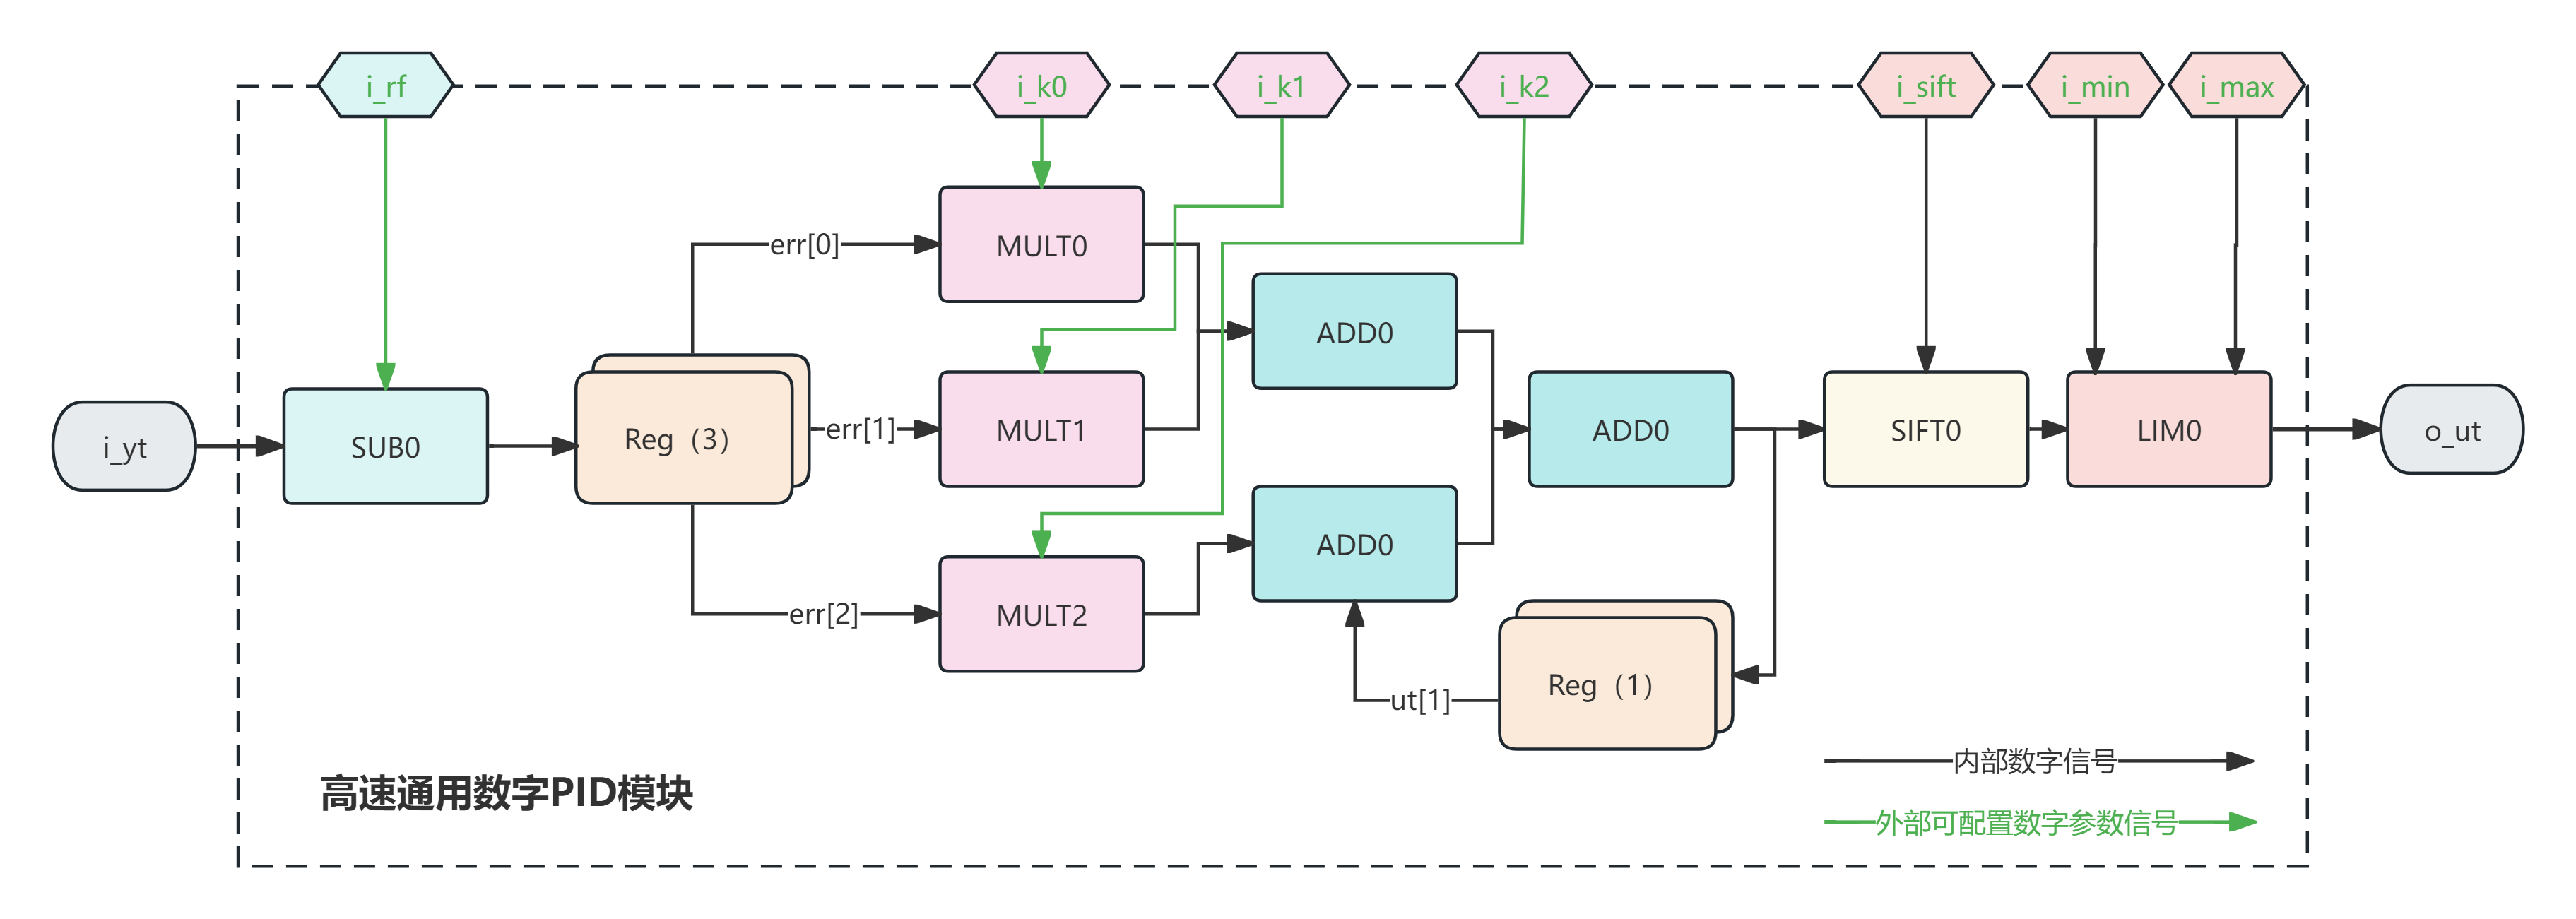
\includegraphics[width=1.0\linewidth]{rtmq/rtmq_pid_structure}
\end{figure}

离散化后的PID表达式为:
\begin{align}
    u(n)=k_p e(n)+k_i\sum_{j=-}^{n}e(j)+k_d[e(n)-e(n-1)]\\
    u(n-1)=k_p e(n-1)+k_i \sum_{j=0}^{n-1}e(j)+k_d [e(n-1)-e(n-2)]
\end{align}

由上面两式可以导出:
\begin{align}
    \Delta u(n)=&u(n)-u(n-1)\\
    =&k_0 e(n)+k_1 e(n-1)+k_2 e(n-2)
\end{align}

其中$k_0=k_p+k_i+k_d,\ k_1=-k_p-2k_d,\ k_2=k_d$,这个式子被称为PID的增量算法。采用这种形式的好处是避免了计算PID原始表达式中的无限积分项。在这种增量式的方式下,PID的控制输出可以表达为:
\begin{align}
    u(n)=u(n-1)+\Delta u(n)=u(n-1)+k_0 e(n)+k_1 e(n-1)+k_2 e(n-2)\label{eq:increment_pid}
\end{align}

按照上述式\eqref{eq:increment_pid}表示的增量式算法,数字PID实现的结构示意图如图\ref{fig:rtmq_pid_structure}所示。接口主要有参考$ref$、参数$k_0, k_1, k_2$、输出移位和限幅$shift, min, max$等可配置输入,反馈信号$y_t$等系统回路输入,以及$u_t$等系统控制输出。用到的器件包括加法器/减法器模块、乘法器模块、寄存器模块。

\subsubsection[高速通用数字PID的FPGA实现]{高速通用数字PID的FPGA实现}

% 增量式PID最终在FPGA中实现的结构图如图\ref{fig:digital_pid_structure_16bits}所示。

根据图\ref{fig:rtmq_pid_structure}所示的结构,可以在FPGA中实现硬件的PID。
其中主要涉及到的数字加法器、数字乘法器,分别采用的是超前进位加法器和Booth乘法器,16位超前进位加法器的FPGA实现结果和16位Booth乘法器的编码和加法树如附录\ref{fig:ahead_adder_16bits}图和图\ref{fig:booth_multiplier_32bits_basic}所示。
对于高速时序电路,尤其是要满足与RTMQ的实时性匹配等相关需求,在开发过程中需要注意流水线的设置和对齐,最终的实现硬件框图如图\ref{fig:digital_pid_structure_16bits}所示,模块端口定义如表\ref{tb:rtmq_pid}所示。
模块首先通过将RTMQ微处理器配置的输入目标参考信号i\_rt和系统的实际输入信号i\_yt作差计算出误差信号err,随后将该误差信号寄存三级,分别为err[0]、err[1]、err[2];接着将三个误差分别与可通过RTMQ微处理器配置的PID系数i\_k0、i\_k1、i\_k2相乘,得到三个结果相加再与上一时刻的输出结果ut[1]相加得到当前时刻的输出;为了避免PID的超调情况下对后续设备的损坏,模块输出最终结果o\_ut前会进行移位(i\_shift)和限幅(i\_min,i\_max),具体参数可以由RTMQ微处理器进行配置。
该高速通用数字PID模块的硬件输出测试和仿真对比如\ref{fig:pid_compare}图所示。从图\ref{fig:pid_compare}中可见,在Vivado中实现的高速PID硬件电路在$k_i=1, k_d=1$的情况下经过大概1000ns后即可以将系统的输出稳定在参考值1000附近,与直接使用MATLAB进行数字PID仿真输出结果基本一致。

\begin{figure}
    \centering
    \caption[16位数字PID的FPGA实现结构图]{16位数字PID的FPGA实现结构图(Vivado)\label{fig:digital_pid_structure_16bits}}
    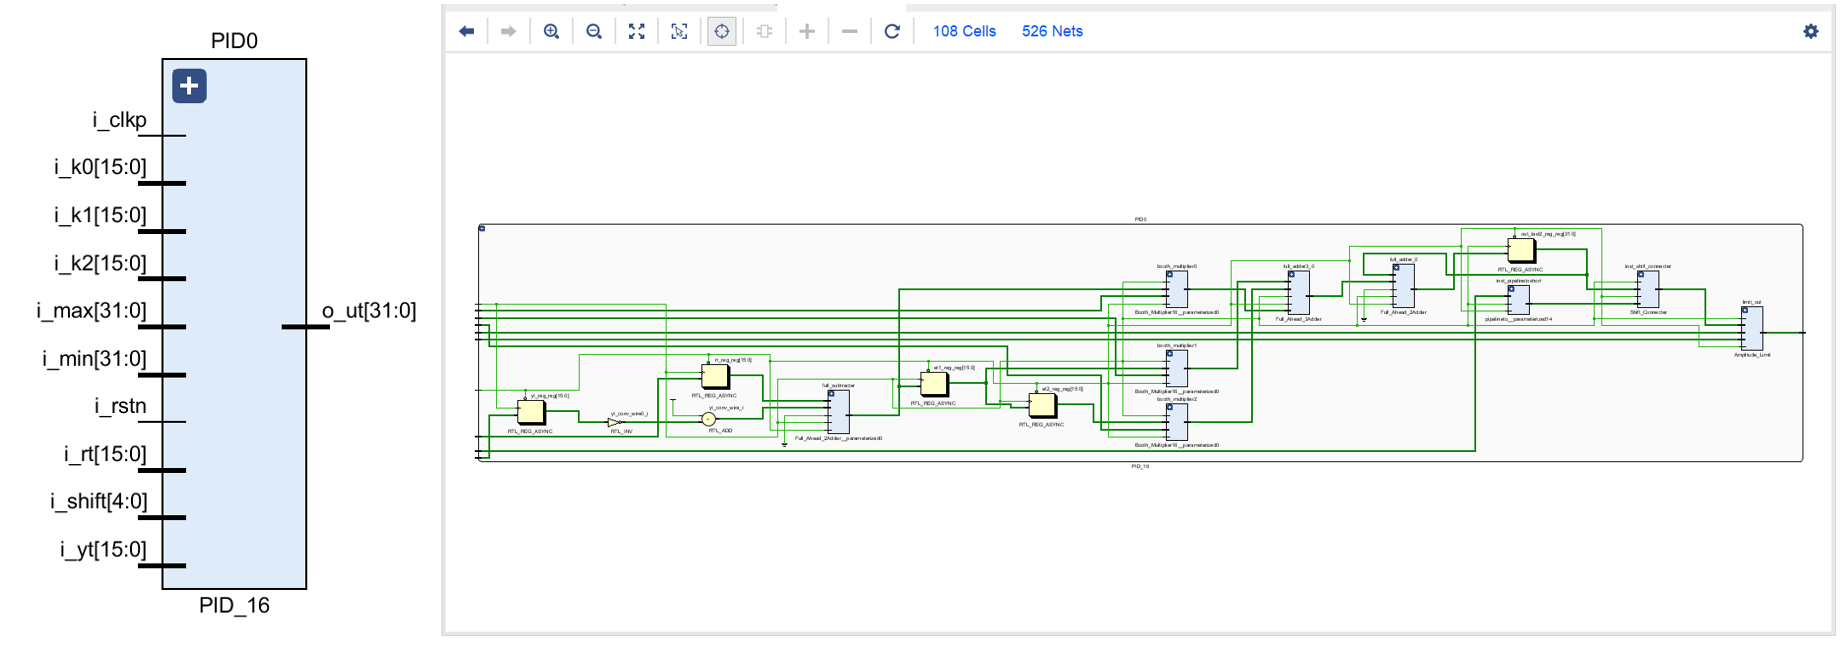
\includegraphics[width=1.0\linewidth]{rtmq/rtmq_pid}
\end{figure}

\begin{table}
    \centering
    \caption[RTMQ系统外设高速通用PID模块端口定义]{RTMQ系统外设高速通用PID模块端口定义\label{tb:rtmq_pid}}    
    \begin{tabular}{L{2.5cm}L{4cm}|L{2.5cm}L{4cm}}
        \toprule
        \multicolumn{2}{c|}{Input} & \multicolumn{2}{c}{Output} \\
        \midrule
        Port & Define & Port & Define\\
        \hline
        i\_clkp         & 系统时钟  & o\_ut[31:0] & PID输出结果 \\
        i\_k0[15:0]     & PID参数k0 &  &  \\
        i\_k1[15:0]     & PID参数k1 &  &  \\
        i\_k2[15:0]     & PID参数k2 &  &  \\
        i\_max[31:0]    & PID输出最高限幅 &  & \\
        i\_min[31:0]    & PID输出最低限幅 &  & \\
        i\_rstn         & PID重置信号 &  & \\
        i\_rt[15:0]     & PID的目标参考信号 &  & \\
        i\_shift[4:0]   & PID输出结果的偏移量 &  & \\
        i\_yt[15:0]     & PID的实际输入信号 &  & \\
        \bottomrule
    \end{tabular}
\end{table}




\begin{figure}
    \centering
    \caption[16位数字PID的FPGA实现结果与仿真结果对比]{16位数字PID的FPGA实现结果与仿真结果对比。初始系统输出$sys$和调节输出$o\_ut$都为0,参考数值$ref$为1000,$k_i=1, k_d=1$,Vivado综合输出时长为3500ns,仿真持续时间为1000$T_c$(系统仿真迭代次数)。\label{fig:pid_compare}}
    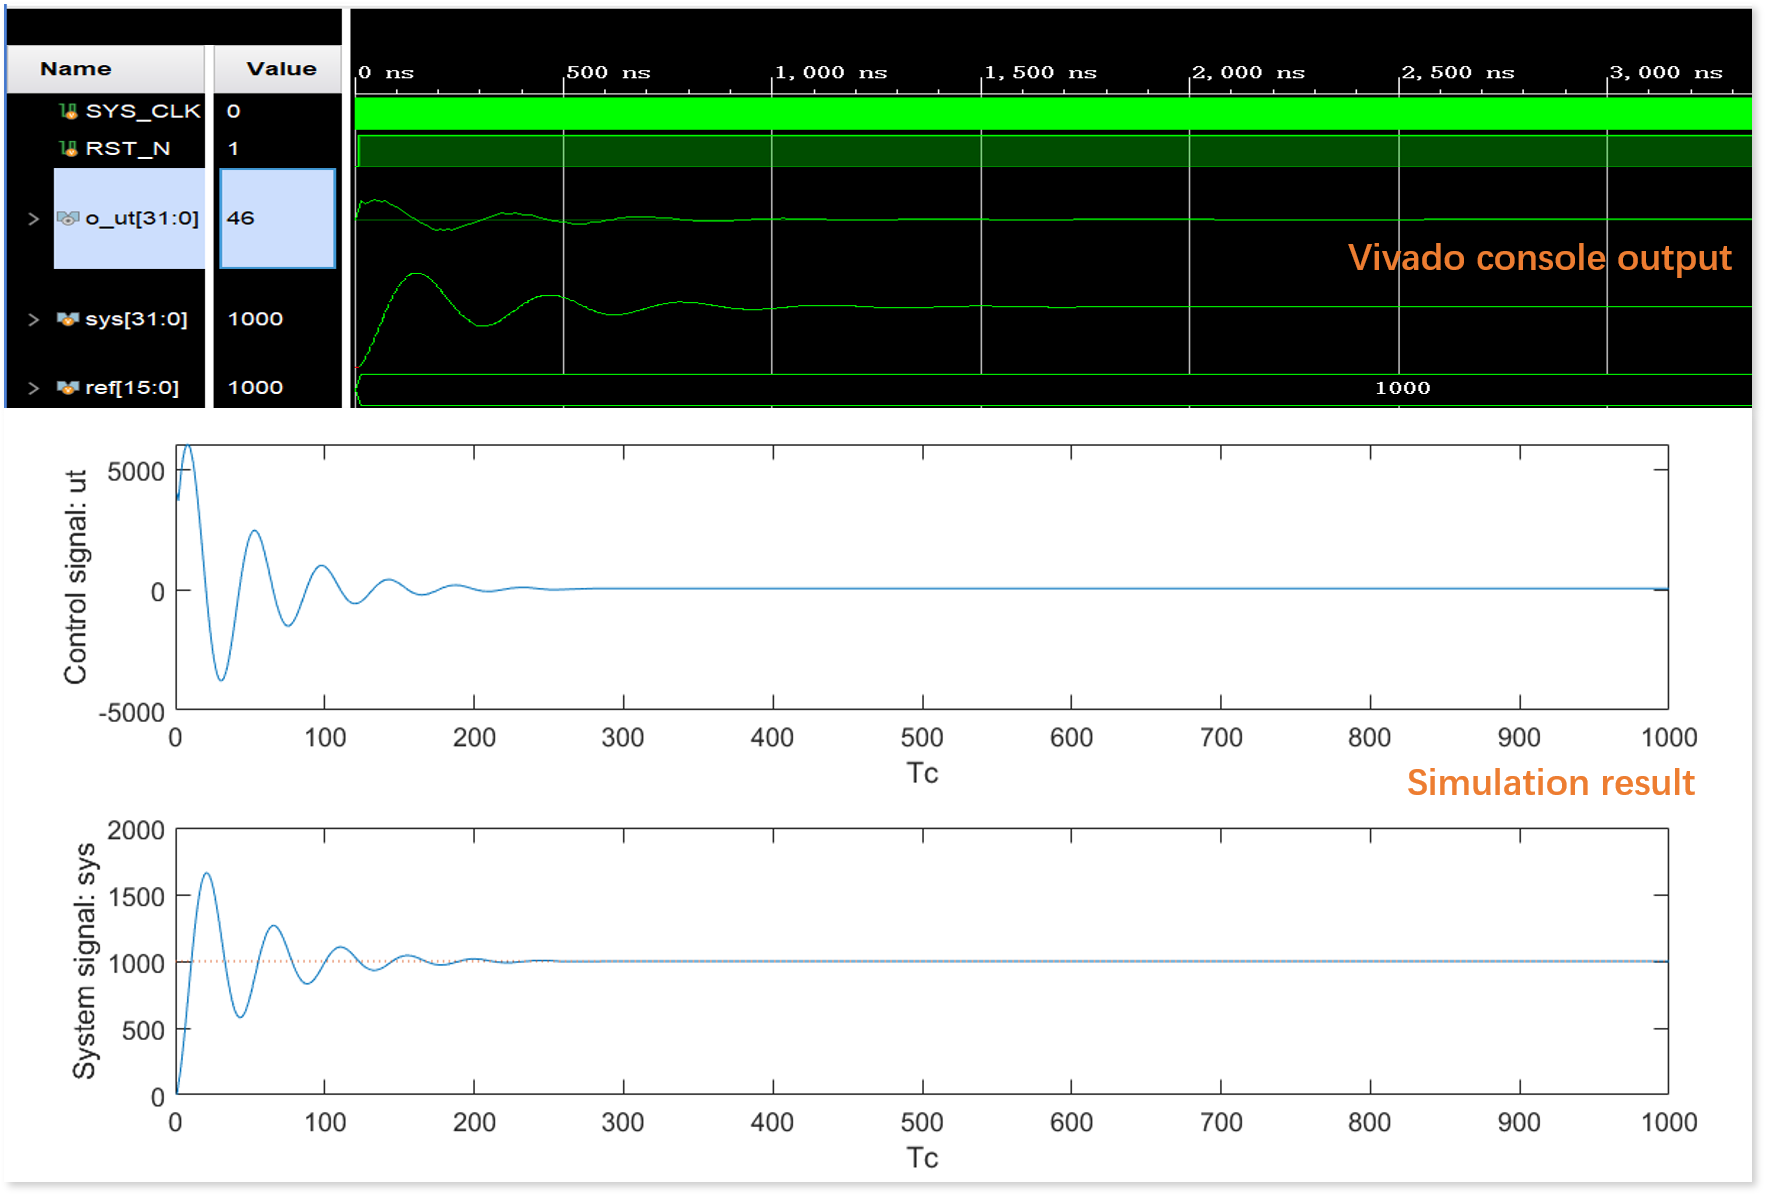
\includegraphics[width=0.8\linewidth]{rtmq/pid_compare}
\end{figure}

整个PID控制器使用了一个减法器、三个加法器、三个乘法器和若干寄存器。图\ref{fig:digital_pid_structure_16bits}是一个16位输入的数字PID,它的输出是32位的,该实例模块总共包含9级流水线,工作频率可达200MHz以上。对更低或者更高位数的数字PID控制器,可以通过替换相应位数的加减运算和乘法模块,并调整相应的寄存器位宽来方便地得到。


\subsection[离子阱频率稳定原理和系统搭建]{离子阱频率稳定原理}


受环境振动和温度变化影响,谐振腔的几何形状,主要是螺旋线的长度和腔体长度会发生变化,进而导致谐振腔的中心频率发生偏移。从谐振腔的S参数图\ref{fig:helical_compares}中可以看出螺线管谐振腔的Q值很大,透过峰较尖锐,即中心频率附近信号透过衰减较大。因此在输入信号频率抖动极小的情况下,受谐振腔中心频率偏移影响,信号的透过幅度将会发生较大的变化。
K. G. Johnson等人\cite[]{Johnson_Wong_Campos_Restelli_Landsman_Neyenhuis_Mizrahi_Monroe_2016}给出了一种采用模拟系统实现的离子阱频率稳定方案,通过采样和整流施加在Paul阱电极上的高压射频信号主动地对离子阱频率进行了稳定。该方案的简化版采用了鉴频器、射频功率放大器、模拟PID控制器、电容分压器、混频器、本地振荡源等器件。采用模拟方案涉及到的器件较多、灵活性差、占用实验空间大,因此我们采用基于RTMQ数字系统的稳定方式来优化上述问题。

\begin{figure}
    \centering
    \caption[基于RTMQ系统的数字PID离子阱频率稳定原理图]{基于RTMQ系统的数字PID离子阱频率稳定原理图。DDS:数字频率发生器;PID:比例微分积分控制器;ADC:模拟数字转换器;$C_1,C_2$:相位同步电容;$C_3,C_4$:射频分压电容。\label{fig:trap_frequency_lock}}
    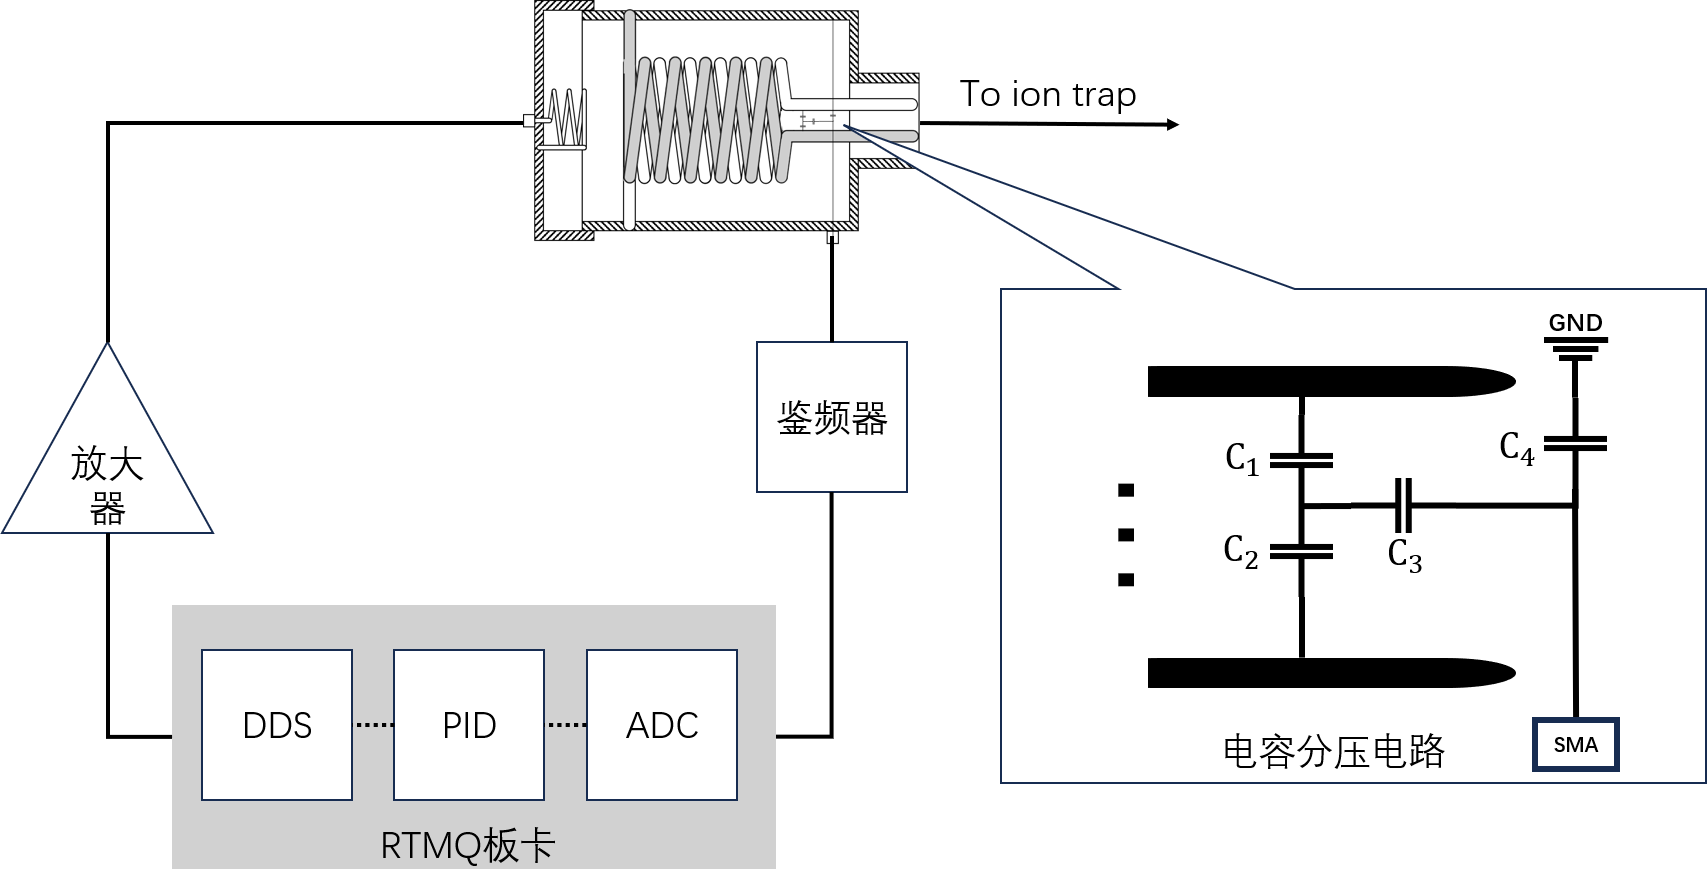
\includegraphics[width=0.9\linewidth]{trap_frequency_lock}
\end{figure}


基于RTMQ系统的离子阱频率稳定原理图如图\ref{fig:trap_frequency_lock}所示。射频信号通过数字PID对DDS进行并行幅度调制产生,随后经过射频功率放大器进入谐振腔耦合输入端。通过调节谐振腔耦合输入端对谐振腔进行阻抗匹配耦合,使得输出功率最大化。随后,在输出端焊接一个射频分压电路,按照100:1的分压比采集射频电压作为检测信号送入鉴频器。接着鉴频器的输出接入RTMQ板卡的16位ADC芯片,进而转换成数字信号作为PID输入,完成整个控制回路闭环。其中,分压电路图如图\ref{fig:trap_frequency_lock}中小图所示,$C_1=C_2\approx10$uF用于同步两个输出端的射频相位;$C_3\approx0.5$pF,$C_4\approx50$pF构成理论上为$100:1$射频分压电路(实际上受到焊接电容影响测得的分压比约为$53:1$)。

\begin{figure}
    \centering
    \caption[DDS输出功率和放大器输出功率]{DDS输出功率和放大器输出功率。横坐标为DDS输出功率(单位dBm),纵坐标为测量得到的放大后的射频功率(单位dBm)。红色空心点是测得的数据点,蓝色虚线为数据点的线性拟合,拟合结果为:$y=0.9644x+32.83$,系数$a=0.9644$接近1表示两者的相关性很好,截距$b=32.83$表示功率放大器的放大数约为32.83dBm。\label{fig:helical_lock_amplifier}}
    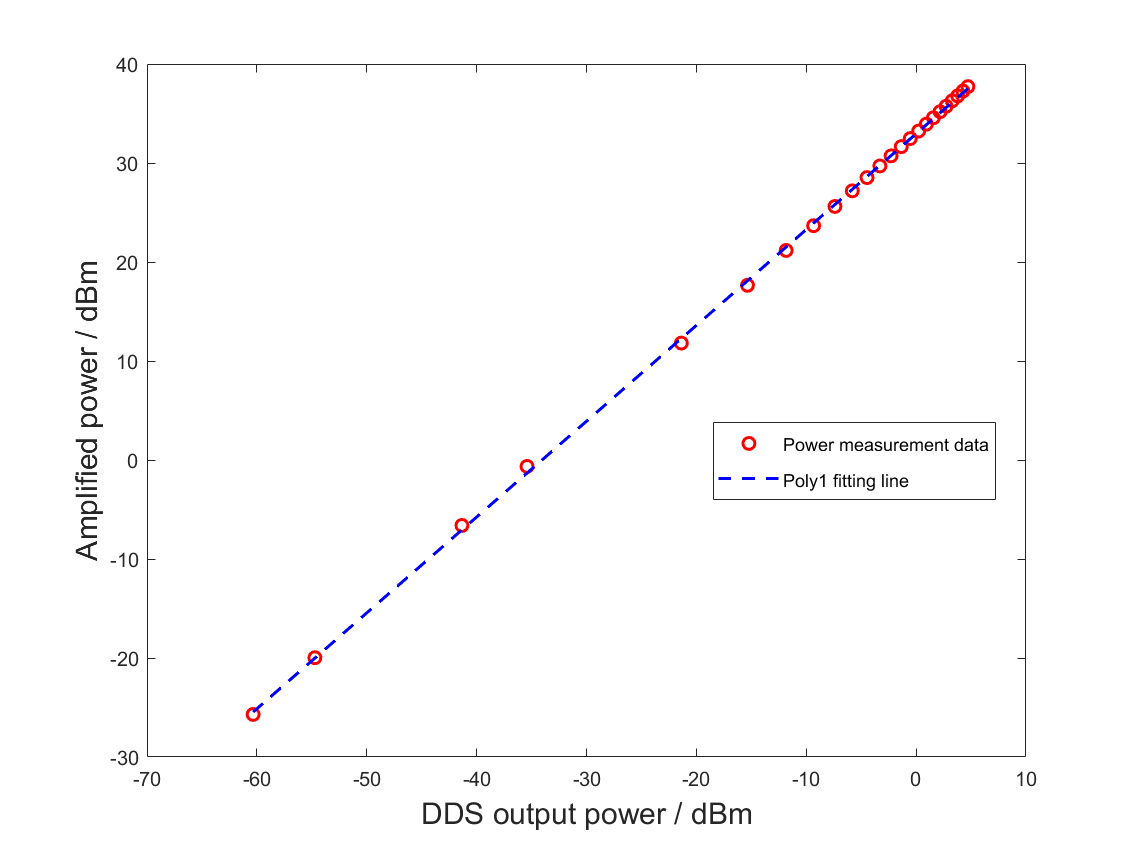
\includegraphics[width=0.8\linewidth]{helical_lock_amplifier}
\end{figure}


\begin{figure}
    \centering
    \caption[阱频稳定系统实验测试图]{阱频稳定系统实验测试图\label{fig:trap_frequency_lock_real}}
    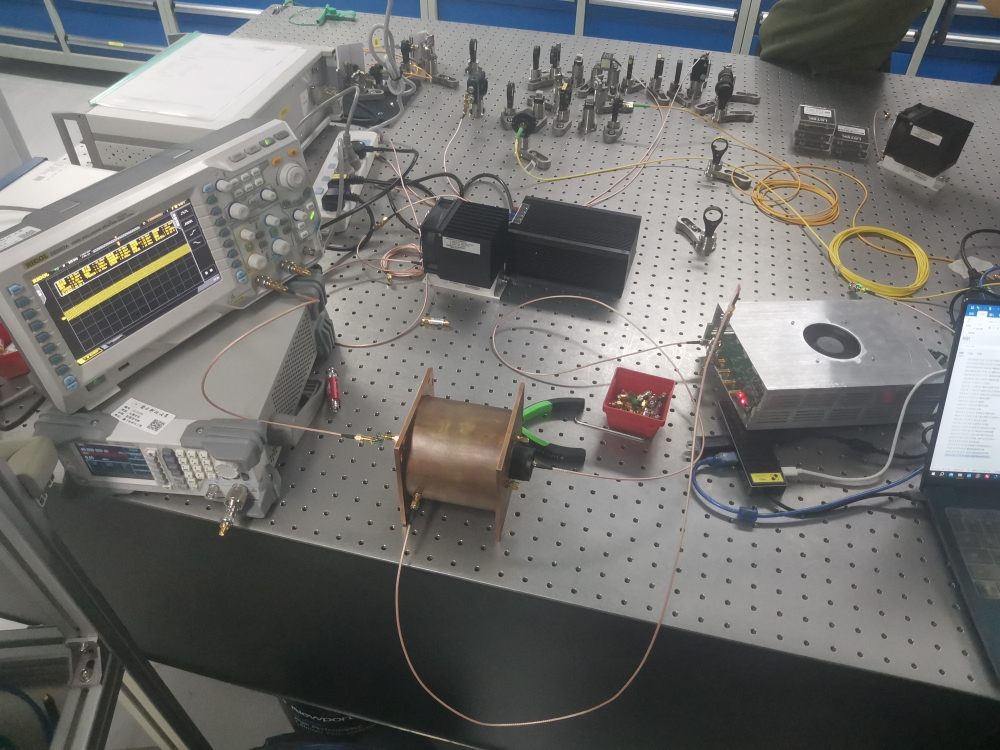
\includegraphics[width=0.9\linewidth]{trap_frequency_lock_real}
\end{figure}


由于系统中需要使用放大器,而放大器对不同频率的信号放大效果有所区别。过大的放大信号可能会损坏谐振腔的分压板,因此这里先用DDS的输出和放大器预先对放大器进行标定,结果如图\ref{fig:helical_lock_amplifier}所示。从结果图中的拟合直线截距上可以看出,在测试范围内输入输出功率关联性很好,信号功率放大器可以对信号放大约32.83dBm。
最终的阱频稳定系统搭建和实验测试图如图\ref{fig:trap_frequency_lock_real}所示。


\subsection[基于RTMQ的离子阱频率稳定系统测试结果]{基于RTMQ的离子阱频率稳定系统测试结果}

\begin{figure}
    \centering
    \caption[阱频稳定本底、稳定前、稳定后原始数据]{阱频稳定本底、稳定前、稳定后原始数据。横坐标:时间(单位s),纵坐标:输出幅度(单位mV)。\label{fig:trap_frequency_lock_original_compare}}
    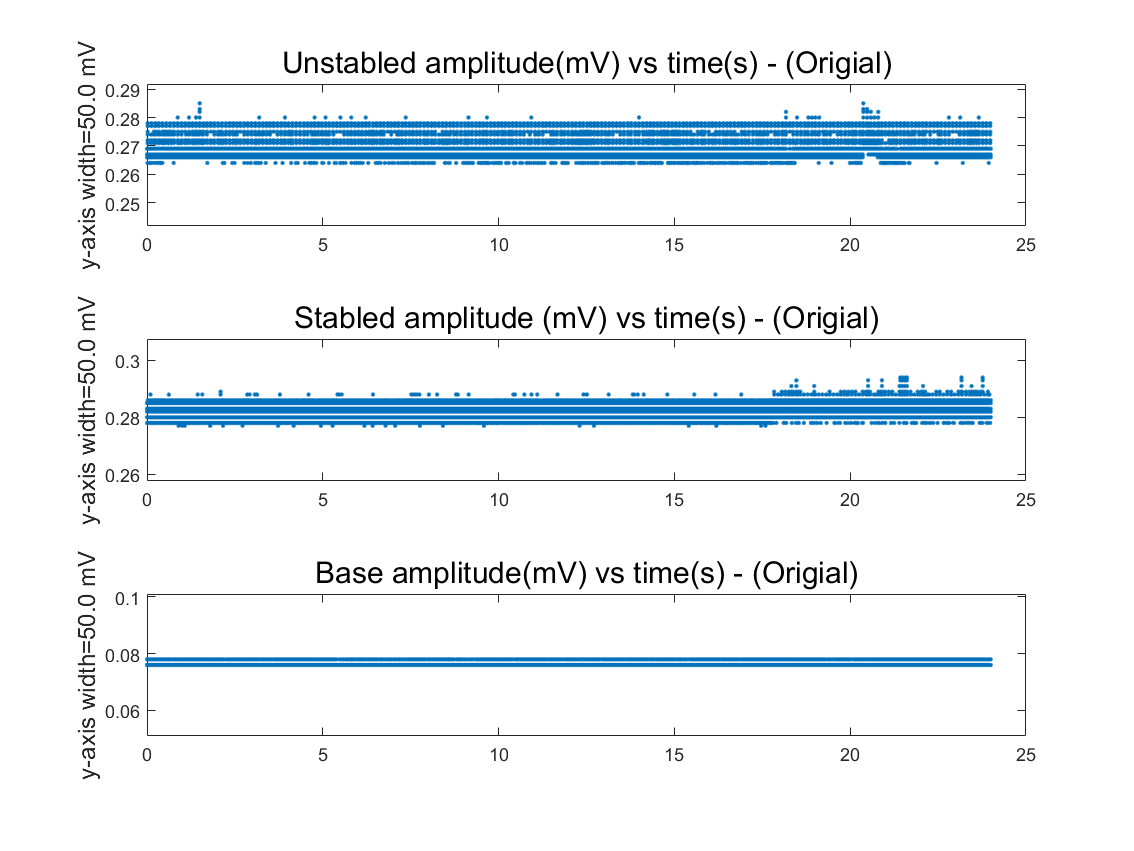
\includegraphics[width=0.8\linewidth]{trap_frequency_lock_original_compare}
\end{figure}



阱频稳定系统实验测试图如图\ref{fig:trap_frequency_lock_real}所示,数据采集使用RIGOL DSG815示波器进行,采样频率为500kHz,采集谐振腔输出信号经过检波器后的幅值$V_0$数据,单位mV,数字PID参数设置为:$k_p=2^5,k_i=1,k_d=0, ref=200$。图\ref{fig:trap_frequency_lock_original_compare}展示了阱频稳定本底(DDS无输出)、稳定前(ADC直连DDS调幅)、稳定后(ADC接PID后连DDS调幅)的原始测量数据,谐振腔的谐振频率为47.25MHz,各组的纵轴宽度居委50mV。从图图\ref{fig:trap_frequency_lock_original_compare}展示的结果来看,稳定前后及本地所处的幅值不完全一致。因此我们首先对结果进行归一化处理$V_{0,norm}=V_{0,original}/mean_{V_{0,original}}$来更好地对比三种情况下的输出稳定性表现,阱频稳定归一化后本底、稳定前、稳定后数据如图\ref{fig:trap_frequency_lock_normed_compare}所示,各组的纵轴宽度均为0.2。从结果中可见,稳定后的结果相对于稳定前的结果有了相对明显的改善。

\begin{figure}
    \centering
    \caption[阱频稳定归一化后本底、稳定前、稳定后数据]{阱频稳定归一化后本底、稳定前、稳定后数据。横坐标:时间(单位s),纵坐标:输出幅度(单位mV)。\label{fig:trap_frequency_lock_normed_compare}}
    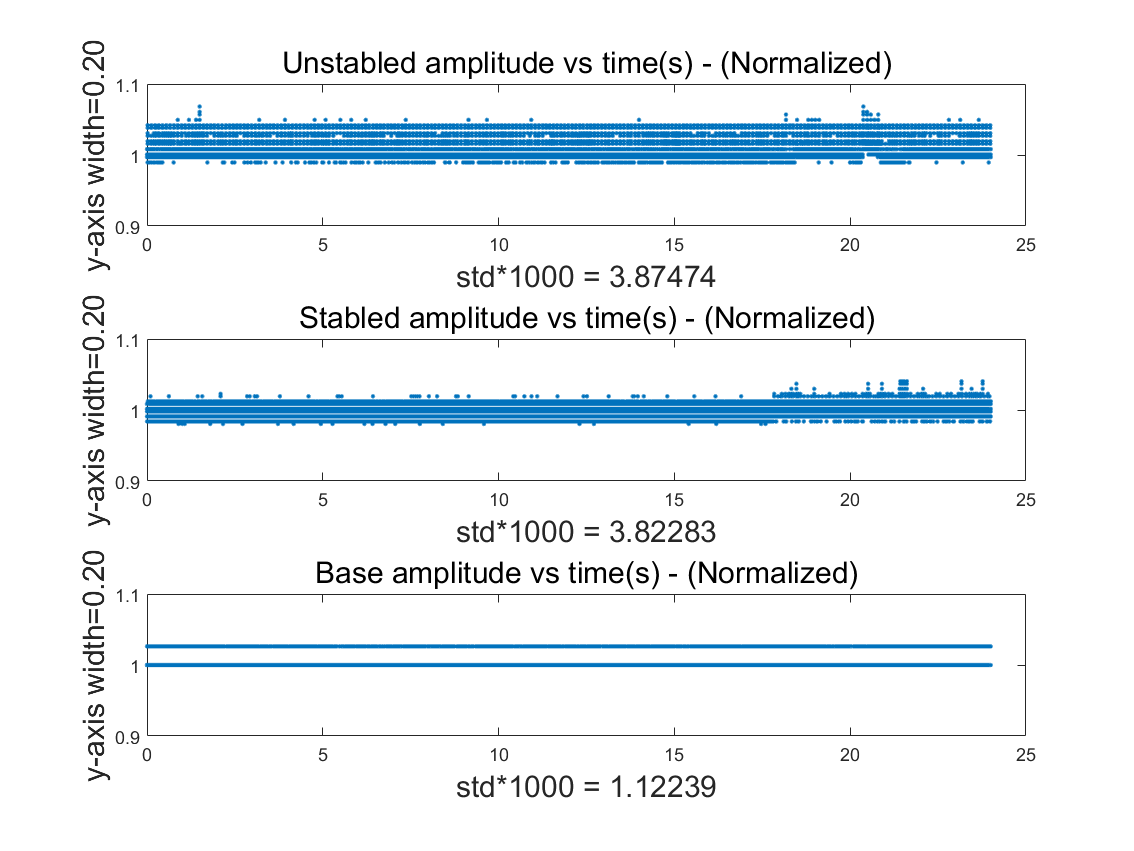
\includegraphics[width=0.8\linewidth]{trap_frequency_lock_normed_compare}
\end{figure}

\begin{figure}
    \centering
    \caption[阱频稳定归一化后本底、稳定前、稳定后数据阿兰方差。]{阱频稳定归一化后本底、稳定前、稳定后数据阿兰方差。数据采样频率:500kHz,横坐标:窗口长度(单位s),纵坐标:阿兰方差(单位1)。\label{fig:trap_frequency_lock_allan_variance_compare}}
    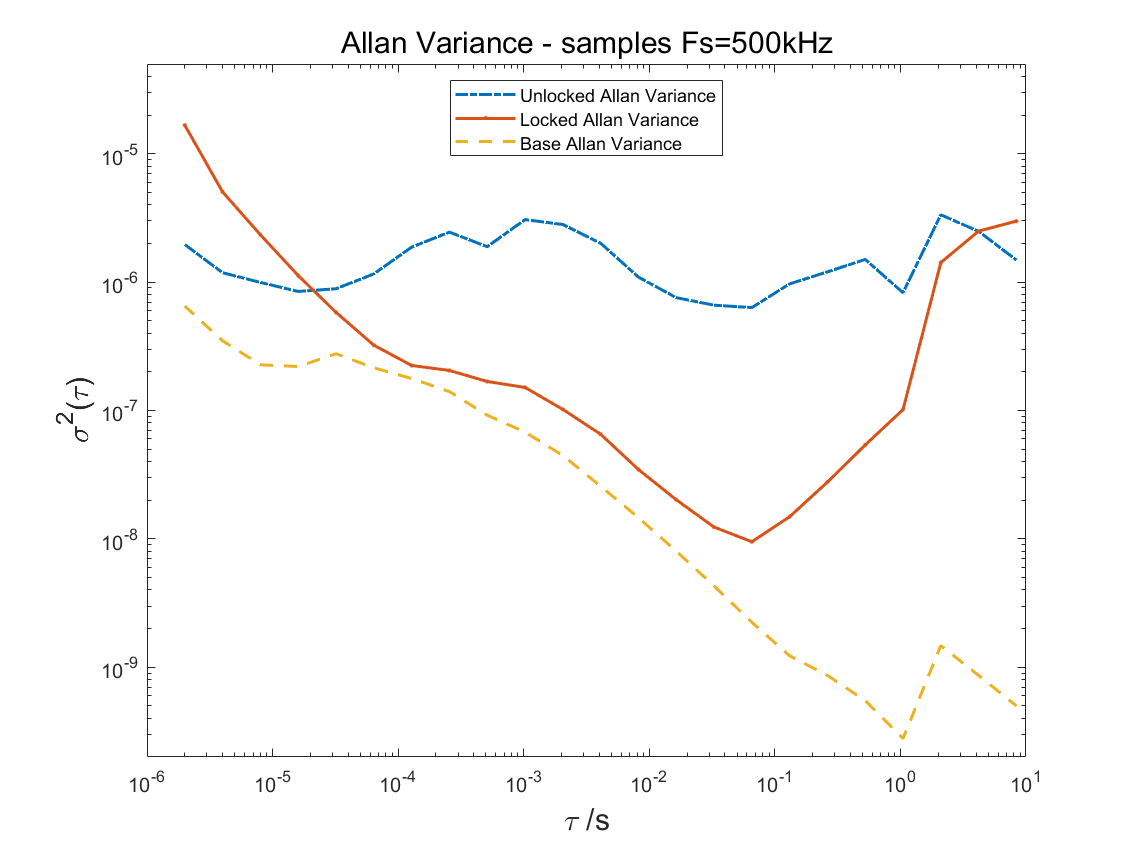
\includegraphics[width=0.8\linewidth]{trap_frequency_lock_allan_variance_compare}
\end{figure}


为了能更好了解稳定效果的整体表现情况,这里绘制出各组数据的阿兰方差。如图\ref{fig:trap_frequency_lock_allan_variance_compare}所示,蓝色点划线为未稳定时的幅值输出情况、橙色实线是使用PID稳定后的幅值输出情况、黄色虚线是幅值输出背景情况。
从图\ref{fig:trap_frequency_lock_allan_variance_compare}中可见,稳定后的性能在时间窗口小于$1.00\times 10^{-4}$s时,也即在100kHz以上的高频段要差于未锁定时的,可见PID稳定的调节作用在高频段引入了噪声。
稳定后的幅值输出性能在时间窗口约为$1.00\times 10^{-4}-1.00$s之间,也即频率为10kHz到直流之间,明显优于未稳定的情况,在时间窗口大于1s时两者性能开始接近,稳定系统对该范围的信号质量能够有明显的优化。
特别的,在时间窗口为$1.00\times 10^{-4}-6.55\times 10^-2$s之间,稳定后的性能接近背景的效果。在时间窗口为$6.55\times 10^-2$时相对于未稳定时的效果最好,有约两个量级的优化。由阱频率的计算公式\eqref{eq:trap_frequency}可知,阱频率$\omega$与谐振腔输出到阱电极上的电压幅值成正比$\omega\sim V_0$,也即在不考虑其它因素的情况下两者的相对标准差$\alpha$一致:$\alpha=\Delta\sigma_{\omega}/\sigma_{\omega}\simeq\Delta\sigma_{V_0}/\sigma_{V_0}$。在单考虑在1kHz附近的噪声干扰的情况下,未锁定时其相对标准差约为$1.80\times10^{-3}$,锁定后的相对标准差约为$3.89\times10^-4$。根据保真度计算公式\eqref{eq:frequency_noise_fidelity},这一因素对于角度翻转$\theta=\pi$的单量子比特操作保真度的影响从稳定前的$1-99.99920\%$降低到了稳定后的$1-99.99996\%$。
% 然而,PID稳定的调节作用在高频段引入了噪声,稳定后的性能在100kHz以上的高频段要差于未锁定时的。

% 典型的镱离子阱频率为$2\pi\times 1$MHz,结合公式和公式可以对





% 阱频稳定系统实验测试图如图\ref{fig:trap_frequency_lock_real}所示,谐振腔输出稳定效果测量结果如图\ref{fig:helical_lock_measure}所示,此时数字PID参数设置为:$k_p=2^4,k_i=1,k_d=0$。l1红色测量数据是在未进行稳定时测的的谐振腔输出幅度与输入功率设定值的关系,l2绿色和l3蓝色测量数据分别为将数字PID控制器目标值设定为-638和-909时的测量结果。在未稳定的情况下,谐振腔的输出幅度会跟随外部输入信号的幅度变化而变化,呈现出一定的比率关系。如图中红色测量数据,其斜率约为244.55;经过稳定后,在大范围内谐振腔的输出幅度仍然会跟随外部输入信号的幅度变化而变化,不过其呈现的比例关系会受到稳定抑制作用而减小,如图中绿色和蓝色测量数据,其斜率在155附近。从中可见,添加数字PID控制器对谐振腔的输出幅度会有明显的稳定抑制作用。

% \begin{figure}
%     \centering
%     \caption[谐振腔输出稳定效果测量结果]{谐振腔输出稳定效果测量结果。数字PID参数设置为:$k_p=2^4,k_i=1,k_d=0$。横坐标为DDS的设定输出功率数字值(非实际功率值),纵坐标我板卡上ADC测得的输出电压数字值(非实际功率值)。该图个数据点测量的是PID参考功率数值一定的情况下,改变输入的射频功率大小,看实际输出功率大小的变化。l1红色线性拟合线:$y=244.55x-1420.9$;l2绿色线性拟合线:$y=154.29x-1118.6$;l3蓝色线性拟合线:$y=157.00x-1279.4$。整体上斜率越小表明控制器对功率大小的变化有抑制作用。\label{fig:helical_lock_measure}}
%     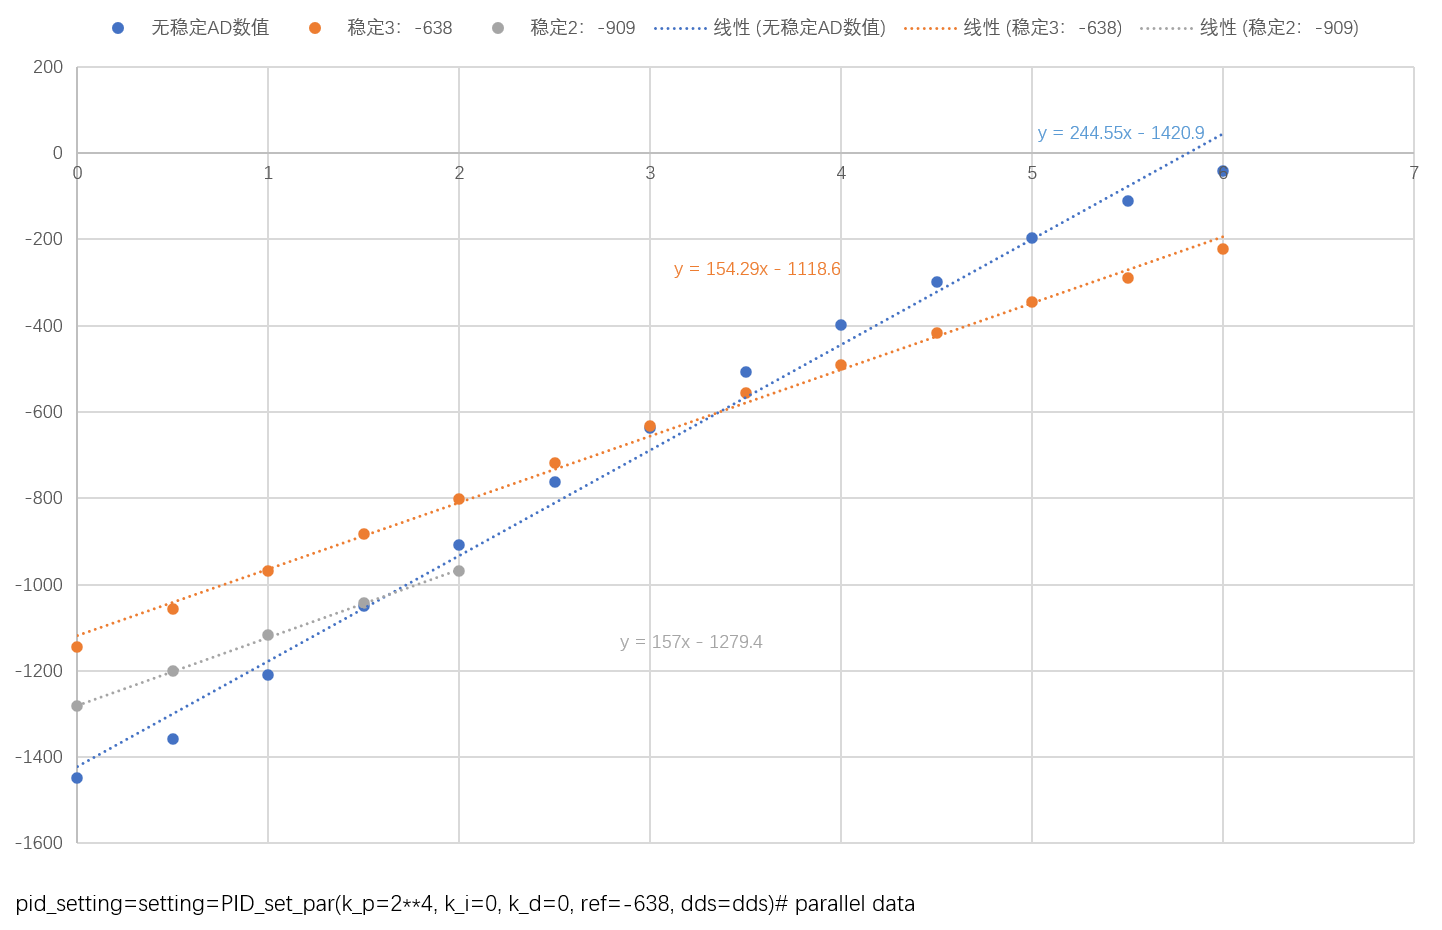
\includegraphics[width=1.0\linewidth]{helical_lock_measure}
% \end{figure}










\newpage
\section[基于RTMQ的激光功率稳定]{基于RTMQ的激光功率稳定\label{section:laser_power_locking}}
% ============================================================================
% ============================================================================
% =======================      激光功率稳定     ===============================
% ============================================================================
% ============================================================================
第\ref{section:quantum_computation}章\ref{section:yb_state_manipulation}节介绍了离子比特的两种操控方式——基于微波和基于激光。由于基于微波的操控在多离子比特情况下寻址困难,实际上对于多比特大规模量子计算的实现通常采用激光方案进行离子比特控制。因此,激光在基于离子的量子计算系统中扮演着十分重要的作用,而激光的功率、频率、相位等重要参数备受重视。其中最基本最重要的是激光的功率稳定,因为激光功率的波动会引入噪声从而影响离子阱中囚禁离子的量子态和量子比特门保真度\cite[]{Blums_Scarabel_Shimizu_Ghadimi_Connell_Händel_Norton_Bridge_Kielpinski_Lobino_et_al_2020}。
% 具体来说,激光功率稳定有以下几个作用:
% \begin{enumerate}
%     \item 提高量子比特的质量:激光功率稳定可以减少离子阱中囚禁离子的运动和量子态的噪声,从而提高量子比特的质量和精度;
%     \item 延长量子比特的寿命:激光功率稳定可以减少离子阱中囚禁离子的能量损失,从而延长量子比特的寿命;
%     \item 提高量子计算的成功率:激光功率稳定可以减少离子阱中囚禁离子的运动和量子态的噪声,从而提高量子计算的成功率;
%     \item 实现精确的量子操作:激光功率稳定可以实现精确的量子操作,例如囚禁离子的冷却、囚禁离子的量子门操作等;
% \end{enumerate}
实验中现有激光功率稳定的系统多是采用模拟PID控制器来进行系统搭建的。使用模拟PID的缺点在于器件成本高、灵活性不好、稳定性差、占用实验台空间大等缺点。本部分将介绍的方案采用RTMQ系统测控板对经典的模拟激光功率稳定系统进行数字化优化替代,使得系统的稳定性、灵活性、集成度等方面有了大幅度的提高。为了抑制如激光功率探测等的数模转换过程中引入到数字系统中的噪声问题,接下来将首先介绍RTMQ的另一个重要的功能外设拓展——高速通用数字IIR滤波器,随后介绍利用RTMQ测控系统结合该数字IIR滤波器和数字PID实现激光功率外部稳定系统的原理及其搭建和测试结果。

\subsection[RTMQ功能拓展高速通用数字IIR滤波器及其FPGA实现]{RTMQ功能拓展高速通用数字IIR滤波器及其FPGA实现\label{section:digital_iir}}
% ============================================================================
% =======================     高速数字滤波器    ===============================
% ============================================================================


在量子计算的实现过程中,对于噪声的抗争从未停止。而对抗噪声的一种十分有效的方式就是使用各种各样的滤波器来对信号进行过滤以提高有用信号的质量。滤波器是本质上一种选频装置,它可以使信号中特定的频率成分通过,而极大地衰减其它频率成分。利用滤波器的这种选频作用,可以进行频谱分析或滤除干扰噪声。
当前实验系统中广泛出现滤波器为模拟滤波器,但是随着量子测控系统的数字化集成化进行逐步加深,在很多内部信号的处理上也有相当多的滤波需求,比如消除ADC芯片采样的噪声等。我们特别地在RTMQ系统板卡上实现了相匹配的高速通用数字IIR滤波器,来丰富RTMQ的功能外设,进一步实现对量子物理实验系统信号的控制和优化。


\subsubsection[无限冲激响应滤波器IIR]{无限冲激响应滤波器IIR}
数字滤波器通过对输入信号进行加工和处理,利用离散系统的特性来改变输入信号的频率特性,从而达到选频、提高信噪比、消除干扰等目的。数字滤波器一般由延迟单元、加法器、乘法器、寄存器等基本运算单元组成。不同类型的数字滤波器有不同的实现方法和应用领域。在通信、语音处理、图像处理、信号处理等领域,数字滤波器都有着广泛的应用。整个离子阱系统中很多模块都有滤波器的需求以获取更高质量的信号来控制量子比特。为此,整个RTMQ系统中需要实现数字滤波器以供系统设计和实现使用。

有限冲击响应滤波器(FIR滤波器)的冲激响应在有限时间内衰减为零,其输出仅取决于当前和过去的输入信号值。FIR滤波器在保证幅度特性的同时,很容易做到严格的线性相位特性。无限冲击响应滤波器(IIR滤波器)的冲激响应理论上应会无限持续,其输出不仅取决于当前和过去的输入信号值,也取决于过去的信号输出值。
FIR滤波器的优点是具有线性相位、稳定性好、容易实现等,缺点是阶数较高时,运算量较大,对存储空间要求较高。IIR滤波器的优点是阶数较低时,运算量较小,对存储空间要求较低,缺点是相位非线性、稳定性较差、设计复杂等。实际滤波器设计经验表明,实现相同形状的滤波效果,IIR滤波器所需的计算资源远小于FIR滤波器。鉴于在FPGA上的算法硬件实现是对资源十分敏感的,因此我们选用IIR滤波器来进行实现。

因它的冲激响应理论上会无限持续而得名,IIR滤波器的输出不仅取决于当前和过去的输入信号值,也受到过去的信号输出值影响,IIR滤波器用差分方程来表示为:
\begin{align}
    y(n)=\sum_{k=1}^Na_ky(n-k)+\sum_{k=0}^Nb_kx(n-k)\label{eq:iir_filter}
\end{align}


其中,$y(n)$表示输出信号,$x(n)$表示输入信号,$a_k$和$b_k$表示滤波器系数。本质上来说,IIR滤波器就是将输入和过去的输出按照某种方式加权计算获得最终输出结果的。对于一个给定阶数和数字位数的IIR滤波器,它的形状完全取决于系数$a_k$和$b_k$。因此,为了维持通用性,在硬件实现的过程中,我们应该把系数($a_k, b_k$)设计为可外部软件配置的。
以四阶为例,通用四阶IIR滤波器的结构框图如图\ref{fig:rtmq_iir_structure}所示,图中$a_0-a_3, b_0-b_3$为IIR滤波器的可配置系数,主要用到的模块有寄存器、Booth乘法器、超前进位加法器等。
\begin{figure}
    \centering
    \caption[IIR滤波器设计结构框图]{IIR滤波器设计结构框图。MULT:Booth乘法器模块;Reg:寄存器模块;ADD:超前进位加法器模块;$i\_filter, o\_filter$:滤波器输入输出信号;$i\_factor\_a,i\_factor\_b$:IIR滤波器参数集合$a_0-a_3, b_0-b_3$输入。\label{fig:rtmq_iir_structure}}
    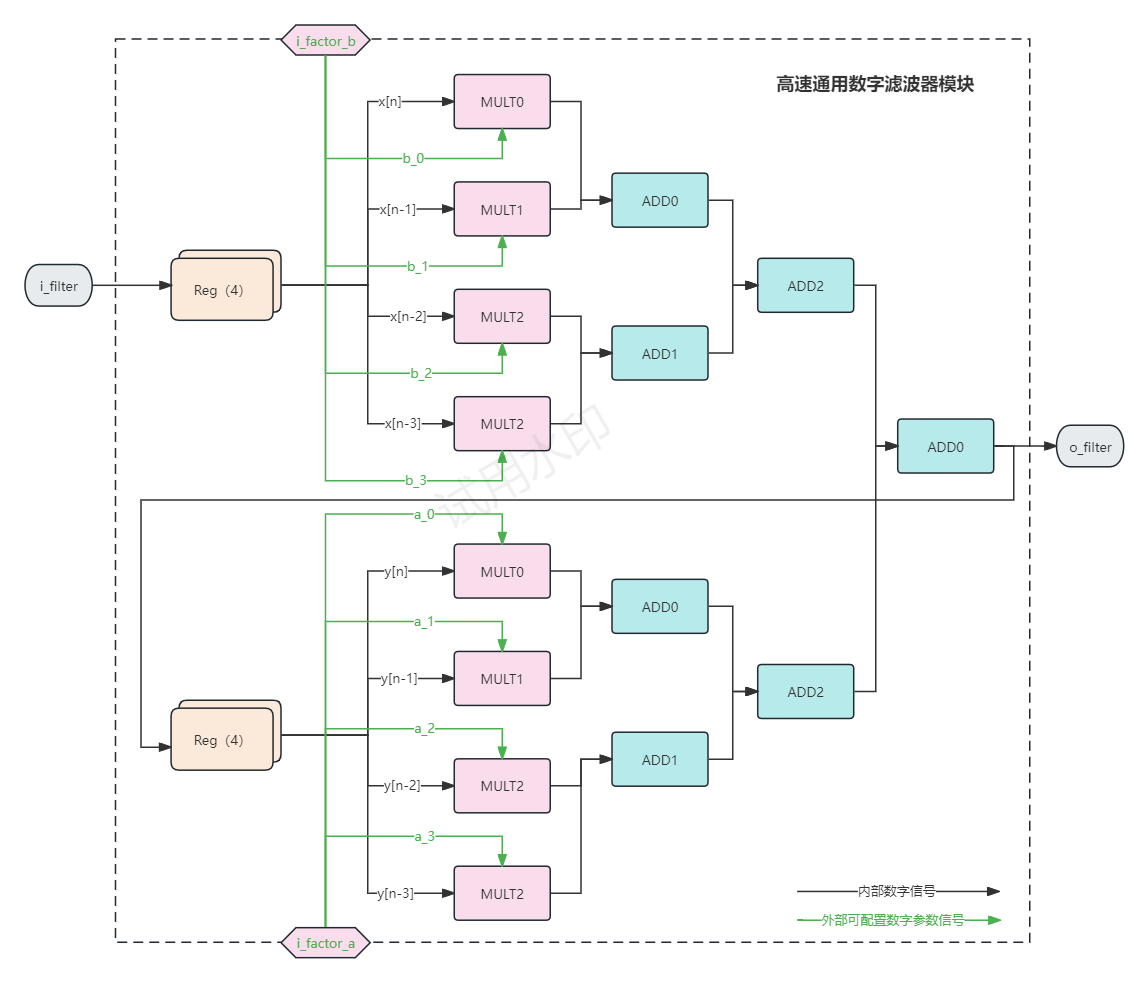
\includegraphics[width=1.0\linewidth]{rtmq/rtmq_iir_structure}
\end{figure}


\subsubsection[高速通用数字IIR滤波器的FPGA实现]{数字IIR滤波器的FPGA实现}

根据图\ref{fig:rtmq_iir_structure}给出的结构图和公式\eqref{eq:iir_filter},可以将其在FPGA中进行实现。该模块的输入为滤波器输入i\_filter,输出为滤波器输出o\_filter,此外还有可外部配置的输出加权参数i\_factor\_a和输入加权参数i\_factor\_b。
滤波器的输入i\_filter经过四级寄存器用于记录x的四级历史输入,分别输出为x[n]、x[n-1]、x[n-2]、x[n-3];随后分别与i\_factor\_b携带的四个参数b\_0、b\_1、b\_2、b\_3相乘得到输入x的加权中间输出,再经过两级加法器得到输入x的加权和输出add\_x。对于滤波器的输出o\_filter也经过四级寄存器记录滤波器的四级历史输出,分别输出y[n]、y[n-1]、y[n-2]、y[n-3];随后分别与i\_factor\_a携带的四个参数a\_0、a\_1、a\_2、a\_3相乘得到输出y的加权中间输出,再经过两级加法器得到输出y的加权和输出add\_y。最后再用一个加法器将add\_x和add\_y相加得到滤波器的最终输出o\_filter。其中i\_factor\_b和i\_factor\_a是滤波器设计的参数,可以根据事先设计好的滤波器形状通过RTMQ微处理器进行外部配置。为了和RTMQ微处理器匹配,该滤波器为有符号整数运算,输入为32位有符号数,输出为32位有符号数。数字IIR滤波器在FPGA中的实现结果的结构图如图\ref{fig:iir_filter_vivado}所示,其模块端口定义如表\ref{tb:rtmq_iir_filter}所示。

\begin{figure}
    \centering
    \caption[IIR滤波器实现结果的结构图]{IIR滤波器实现结果的结构图(Vivado)\label{fig:iir_filter_vivado}}
    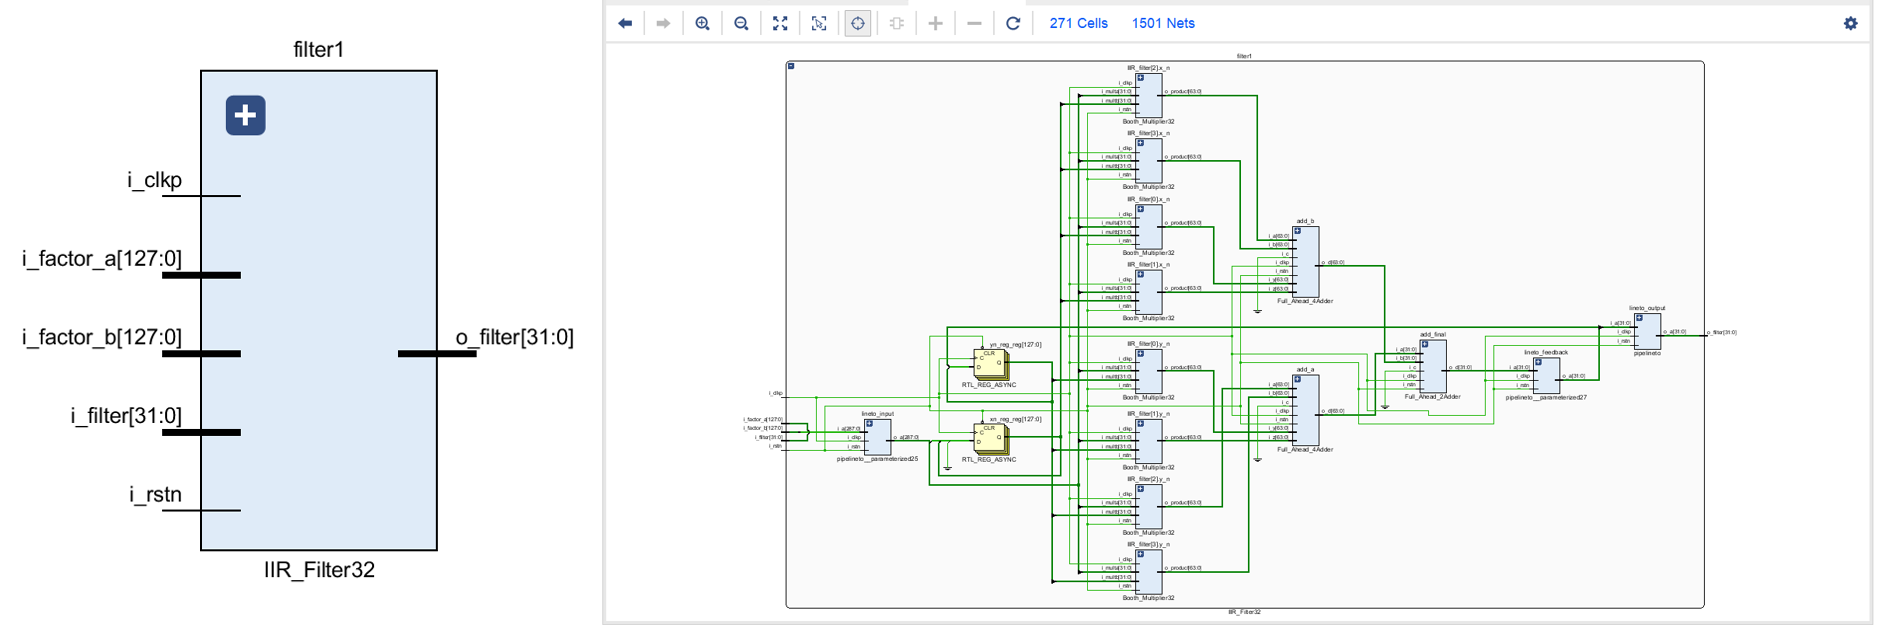
\includegraphics[width=1.0\linewidth]{rtmq/rtmq_iir_filter}
\end{figure}

需要注意的是
% 在极端情况下,该滤波器模块中的加法器模块计算过程中可能有溢出情况,为了避免这种情况可以考虑和数字PID类似在滤波器输入前添加数字限幅器。另外
为了应对滤波器参数为小数的情况,在本设计中将滤波器参数首先乘以$2^{n}$放大后再作为参数赋值给i\_factor\_a和i\_factor\_b,然后再将滤波器运算结果进行n位右移缩小回来(例如n=24)用于输出和迭代。为了匹配乘法器和RTMQ微处理器核心的位宽,反馈和输出时将经过乘法器和加法器后计算的64位输出结果转换为32位作为o\_filter。
除此之外,由于上一时刻的输出结果$y(n-1)$需要参与到下一时刻的输出结果的计算中,因此从计算结果o\_filter到y迭代反馈之间仅能有一级流水线存在,否则输出结果就会出错。也即从乘法器输入到乘法器输出,以及加法器输入到加法器输出并反馈到乘法器输入这个回路中只能存在一级流水线,在本设计中该级流水线按插在输出最终结果的最后一级加法器模块之后。正因此,这个IIR滤波器无法工作在太高的频率上,需要在板上额外配置工作频率,本设计中该32位通用IIR滤波器在FPGA板上的工作频率为25MHz。


\begin{table}
    \centering
    \caption[RTMQ系统外设高速通用PID模块端口定义]{RTMQ系统外设高速通用PID模块端口定义\label{tb:rtmq_iir_filter}}    
    \begin{tabular}{L{3cm}L{3.5cm}|L{2.5cm}L{4cm}}
        \toprule
        \multicolumn{2}{c|}{Input} & \multicolumn{2}{c}{Output} \\
        \midrule
        Port & Define & Port & Define\\
        \hline
        i\_clkp             & 系统时钟 & o\_filter[31:0] & 滤波器输出 \\
        i\_factor\_a[127:0] & 四阶滤波器参数a0[31:0]-a3[31:0] &  &  \\
        i\_factor\_b[127:0] & 四阶滤波器参数b0[31:0]-b3[31:0] &  &  \\
        i\_filter[31:0]     & 滤波器输入 &  &  \\
        i\_rstn             & IIR重置信号 &  & \\
        \bottomrule
    \end{tabular}
\end{table}







\subsubsection[滤波器形状测量]{滤波器形状测量}
数字滤波器的形状设计可以采用MATLAB中的滤波器设计器来完成。在量子计算的实验系统中常常要应对的是高频信号噪声,低通滤波器是十分常见的需求,因此下面以低通滤波器为例进行说明。通过MATLAB设计一个巴特沃斯型迭代滤波器,具体设计指标为:采样频率$f_s=200$MHz,通带截止频率$f_p=100$kHz,阻带截止频率$f_s=2$MHz,通带允许最大衰减$d_p=3$dB,阻带允许最大衰减$d_s=50$dB。结果为一个3阶的迭代滤波器,参数为:
$
a_0=1.0000;
a_1=-1.9950;
a_2=0.9950;
a_3=0;
b_0=0.3115\times 10^{-5};
b_1=0.6231\times 10^{-5};
b_2=0.3115\times 10^{-5};
b_3=0$
由于a参数和b参数两者均为浮点数,无法直接赋值到数字IIR滤波器中。因此需要对系数输入进行放大处理,然后在滤波器结果迭代和输出时再缩放回来完成计算。将设计系数结果放大$2^{24}$后并取整为:
$a_0=16777216;
a_1=-33470572;
a_2=16693565;
a_3=0;
b_0=52;
b_1=105;
b_2=52;
b_3=0$。



带宽的测量采用外部射频源输出一系列频率到板上ADC(16位),然后将ADC的输出作为IIR滤波器的输入,采集ADC输入的数字信号幅值$o_{adc}$和滤波器输出的数字信号幅值$o_{filter}$,将两者的幅值相比得到滤波器增益$G=o_{filter}/o_{adc}$,进而绘制出测量得到的滤波器形状。实际测量得到的滤波器形状和直接模拟运算得到的滤波器形状结果如图\ref{fig:filter_design_real1}。可以看到设计的理论截止频率(100kHz)和数字滤波器实际的截止频率(13.17kHz)有较大的差异。其原因主要有一下几方面:
\begin{itemize}
    \item 数字滤波器的设计实际上是对模拟滤波器的近似,因而结果不绝对准确;
    \item 实际赋值到数字PID中的滤波器设计参数存在数据截断;
    \item 实际在FPGA中的硬件滤波器运算位宽有限,迭代过程中存在数据截断;
    \item 频谱测量过程中用到ADC(16位)等中间数字过程,对数字信号幅值数据的表征不够精确。
\end{itemize}

在理论结果绘制中,对滤波器的参数进行类似FPGA硬件中的人工截断,得到的模拟结果如图\ref{fig:filter_design_real2}所示。可见此时理论设计的截止频率结果与实际硬件数字PID的截止频率结果更加接近了。尽管仍然存在一定的差异,已经可以给出比较有意义的指导信息了。整体上来看,硬件实现的数字滤波器在配置为低通滤波器的时候带宽会被压窄。因此如果需要100kHz的带宽,则需要在设计时适当放大这个带宽需求。最终实际的滤波器带宽可以通过测量来进一步验证是否符合使用要求,如果不符合则可以重新设计和测试。值得一提的是,在实现了通用的硬件IIR滤波的基础上,重新设计和配置$a_0-a_3, b_0-b_3$等参数是十分方便快捷的,仅需更改可配置寄存器的值即可。

\begin{figure}
    \centering
    \caption[IIR滤波器设计仿真和实际测试结果]{IIR滤波器设计仿真和实际测试结果\label{fig:filter_design_real1}}
    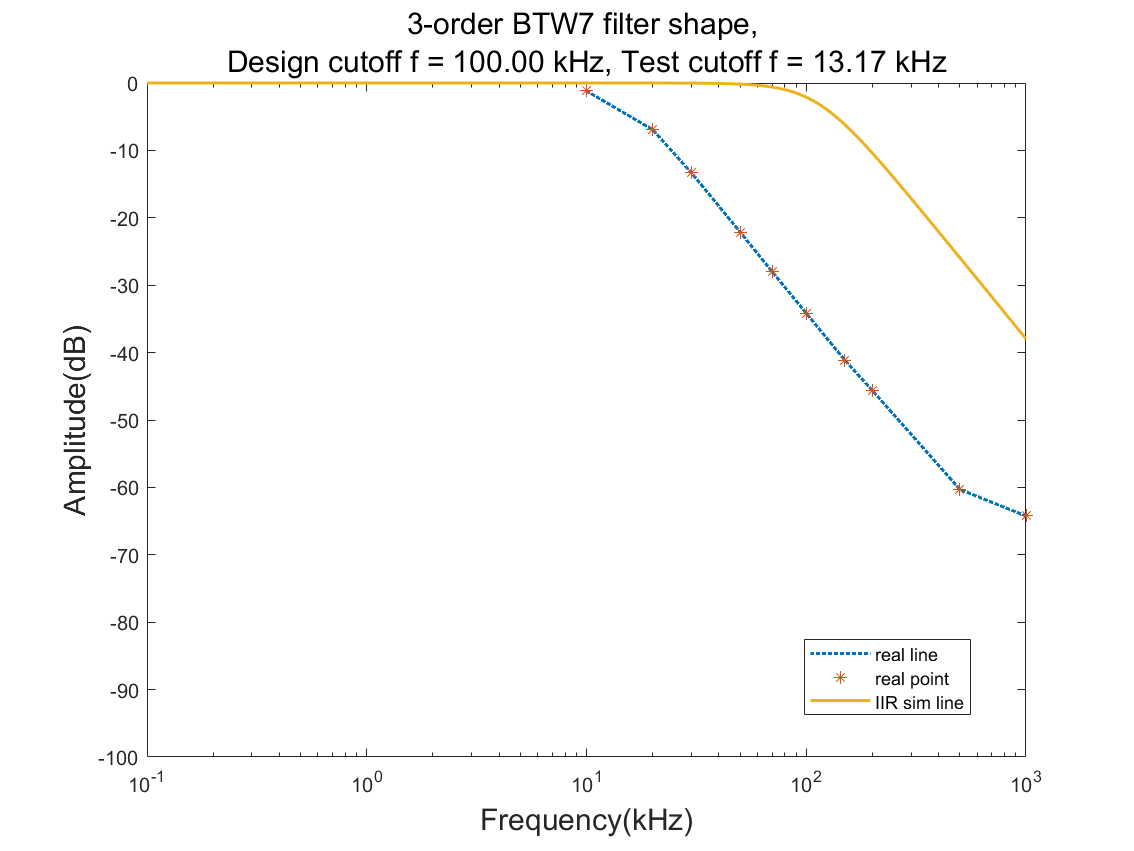
\includegraphics[width=0.8\linewidth]{rtmq/filter_design_real1}
\end{figure}

\begin{figure}
    \centering
    \caption[IIR滤波器考虑截断的仿真和实际测试结果]{IIR滤波器考虑截断的仿真和实际测试结果\label{fig:filter_design_real2}}
    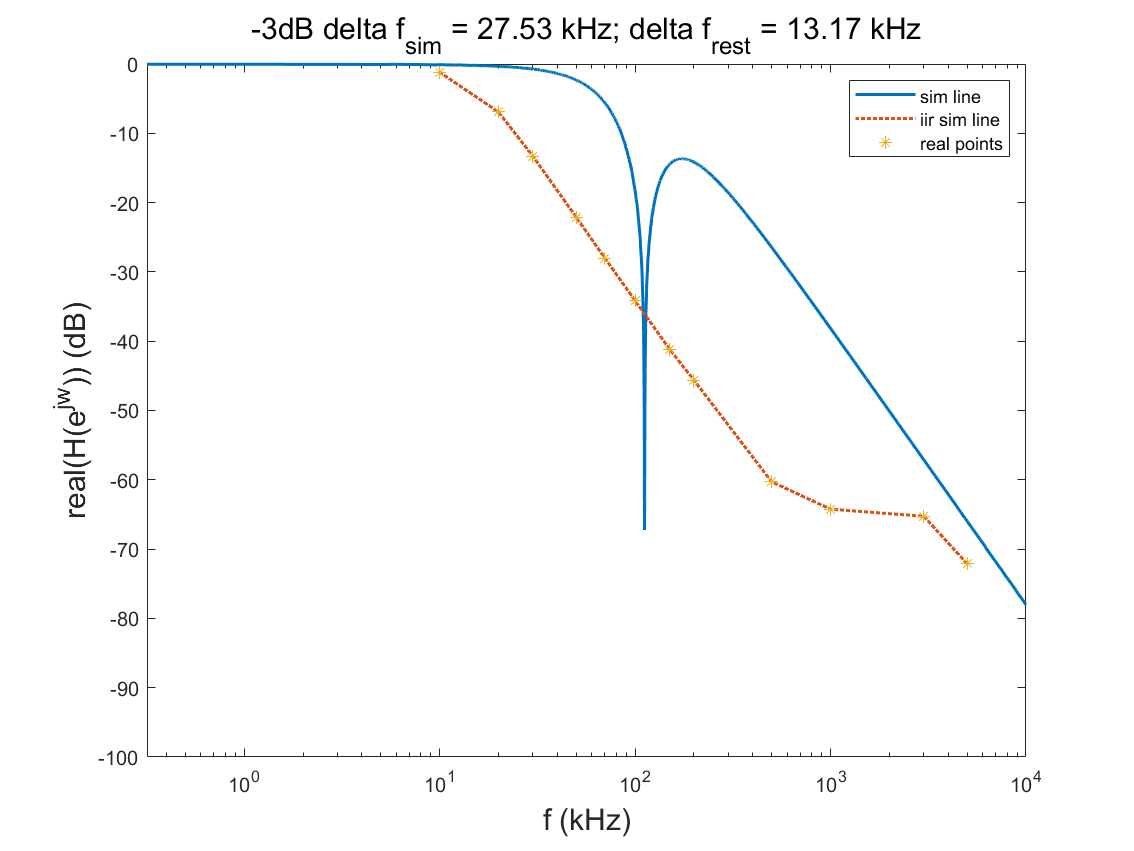
\includegraphics[width=0.8\linewidth]{rtmq/filter_design_real2}
\end{figure}

% \newpage
\subsection[激光功率外部稳定原理和系统搭建]{激光功率外部稳定原理和系统搭建}
激光功率稳定与多种因素有关,通常来说有温度控制、电流控制、光学反馈控制、机械稳定性等,这些因素基本都针对激光器本身进行稳定。除了对激光器本身进行稳定外,还可以激光输出的后续光路中设计相关的控制系统对激光进行稳定。这种方式独立于激光器吱声的出光稳定,可以在激光出光稳定的基础上进一步提高激光功率的稳定性。下面介绍这种激光功率外部稳定原理和实现。

\begin{figure}
    \centering
    \caption[激光功率外部稳定]{激光功率外部稳定。HWP:半波片,PBS:偏振片,PS(B):光功率分数器,AOM:声光调制器,PD:光功率探测器,ADC:数模转换器,IIR:无限冲激响应滤波器(配置为低通),PID:比例微分积分控制器,DDS:数字频率生成器、PA:功率放大器、PS(RF):射频功率分数器。\label{fig:laser_stabilization0}}
    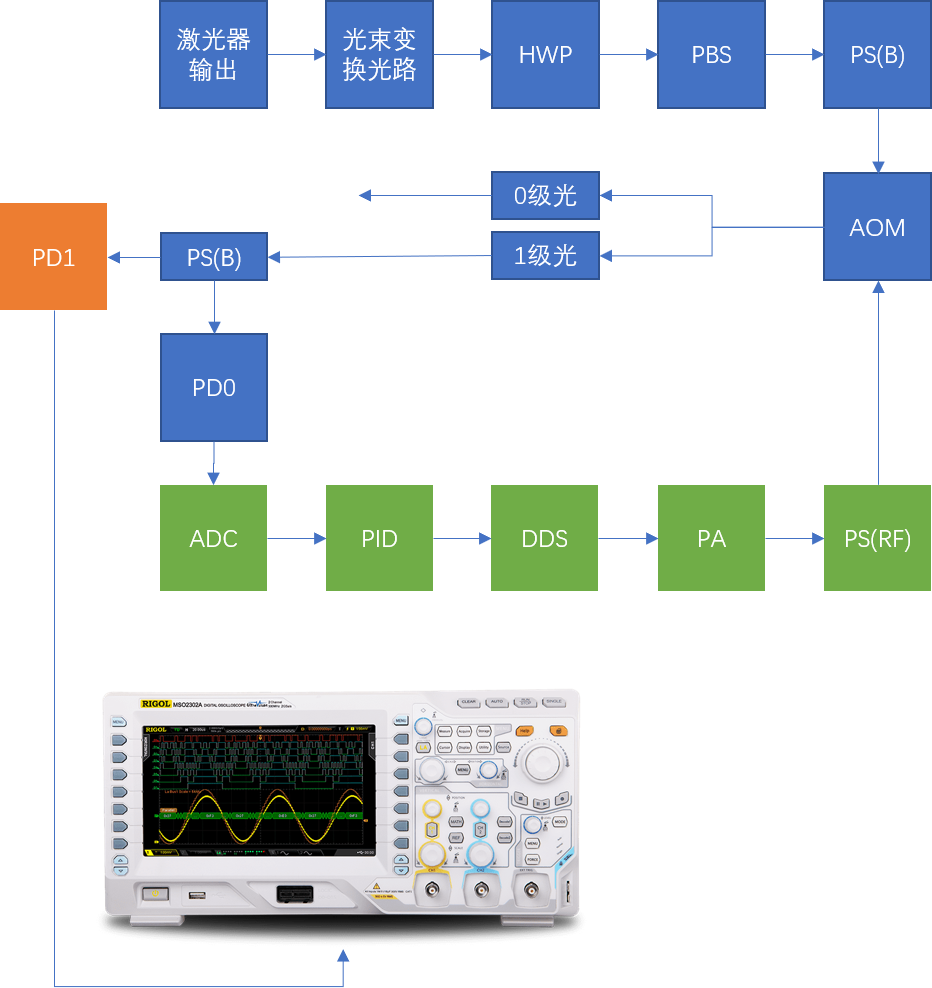
\includegraphics[width=1.0\linewidth]{laser_stabilization0}
\end{figure}

激光功率外部稳定系统主要包括如图\ref{fig:laser_stabilization0}几部分:435nm激光器、透镜组、半波片HWP、光偏振分束镜PBS、光功率分配镜PS(B)、声光调制器AOM、光分束镜PS(B)、光子探测器PD、ADC芯片、高速通用数字PID、高速通用数字无限冲激响应滤波器IIR、直接数字信号合成器DDS、射频功放PA、射频功率分配器PS(RF)。

整个过程如下,首先激光器产生激光经过透镜和反光镜组将激光变换到要求的光斑大小和入射位置;接着使用半波片(HWP)将光转化为垂直和水平偏振成分;接着使用偏振分数器将偏振光提纯为匹配AOM偏振需求的光;随后使用光功率分配器分出一部分激光用于构成反馈回路,另一部分光经过控制回路控制的AOM调制后成为可用的功率稳定激光;激光经过AOM后会产生若干级衍射光,起中主要能量集中在0级和1级衍射光上,我们可以选择其中一路来进行探测和稳定(这里选择1级光);将一级光经过光功率分束镜一部分作为测试监测,另一部分用于反馈控制回路中。控制器采用基于RTMQ板卡数字系统实现,主要器件为ADC、PID、IIR、DDS,除此之外还需要功率放大器(PA)和射频功率分配器(可选,如果只有一路则不用,实际使用中可以分出多路来调控多了AOM)。
RTMQ测控板控制器系统工作如下:
\begin{enumerate}
    \item 1. 首先板上ADC芯片将用PD探测到的激光功率转化为16位无符号数字信号,为了与后续的16位有符号器件相匹配,这里对ADC芯片给出的无符号数映射为有符号数;
    \item 2. 上步的ADC输出经过IIR滤波器,IIR滤波器的形状设计约为0-100kHz低通滤波,用以排除一些高频噪声;
    \item 3. 经IIR滤波器滤波后进入PID,PID的k0,k1,k2参数用python脚本由kp,ki,kd自动转换得到,实验中常用的典型值为:kp=100,ki=2,kd=0;
    \item 4. 接着PID的输出直接用来调控DDS,对DDS进功率调制,这里为了实现更快的反馈DDS配置为并行幅度调制模式(该模式下DDS射频信号输出幅度由16位有符号数决定,因此在PID直接输出进入DDS前要再加上一个基础功率信号值,该信号值应接近目标稳定功率对应的功率信号值)。
\end{enumerate}

\begin{figure}
    \centering
    \caption[激光功率稳定系统测试图]{激光功率稳定系统测试图\label{fig:laser_stabilization_real}}
    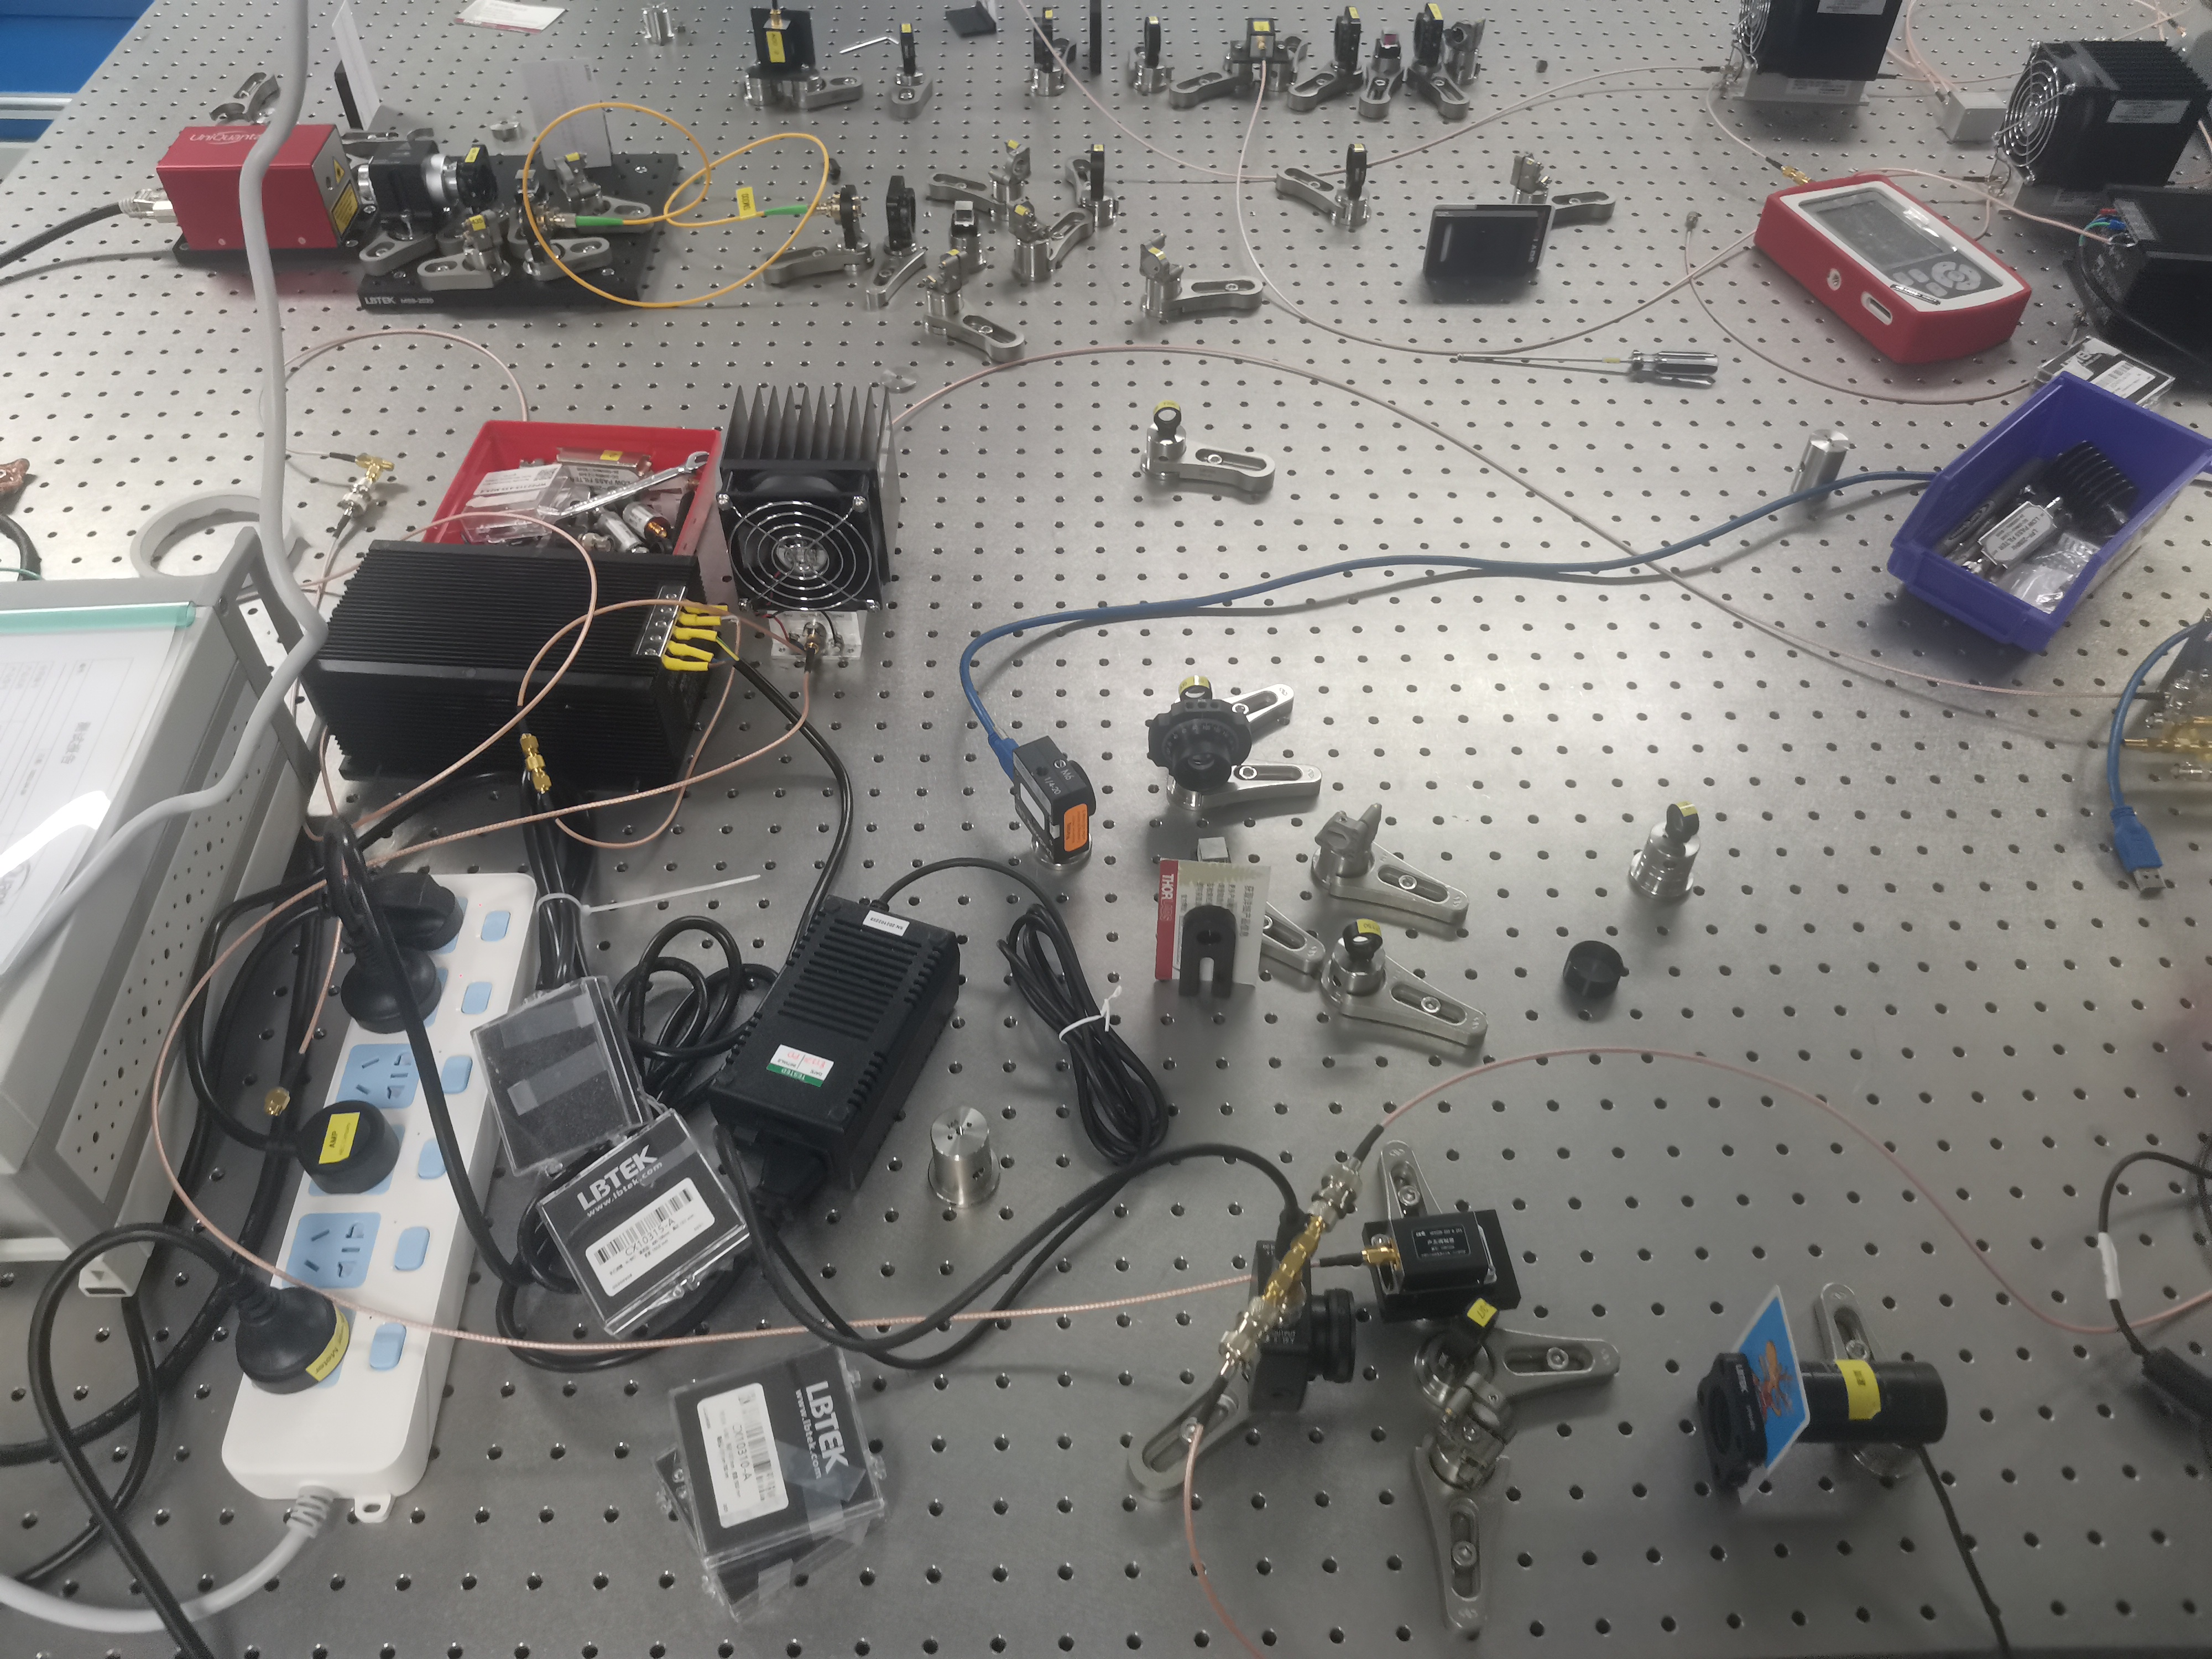
\includegraphics[width=0.8\linewidth]{laser_stabilization_real}
\end{figure}

通过调节射频功率的大小可以控制AOM1级光和0级光的功率分布,在合理范围内,射频功率越大1激光分得的功率越高。数字PID根据1级衍射光的功率变化控制DDS输出不同功率的射频信号,从而实现对1级衍射激光的稳定控制。对于整个控制回路,一般来说只需要分出两路如AOM0和AOM1,一路AOM0用来做功率稳定的反馈回路,另一路AOM1用来做工作光,然后可以拓展地在另一路后面添加光功率分配镜来获得更多路的稳定光,如附录图\ref{fig:laser_stabilization}所示。
激光功率稳定系统实验测试如图\ref{fig:laser_stabilization_real}所示。




\subsection[基于RTMQ的激光功率稳定系统的测试结果]{基于RTMQ的激光功率稳定系统的测试结果}
% D:\Database\Files\2021-2024-研究生事件文件\2022-2023\研究\2023年4月13日-光功率稳定\2023年4月27日_光功率计测试数据

\begin{figure}
    \centering
    \caption[激光功率外部稳定原始数据]{激光功率外部稳定本底、稳定前、稳定后原始数据。横坐标:时间(单位um),纵坐标:功率(单位uW)。\label{fig:laser_stabilization_data}}
    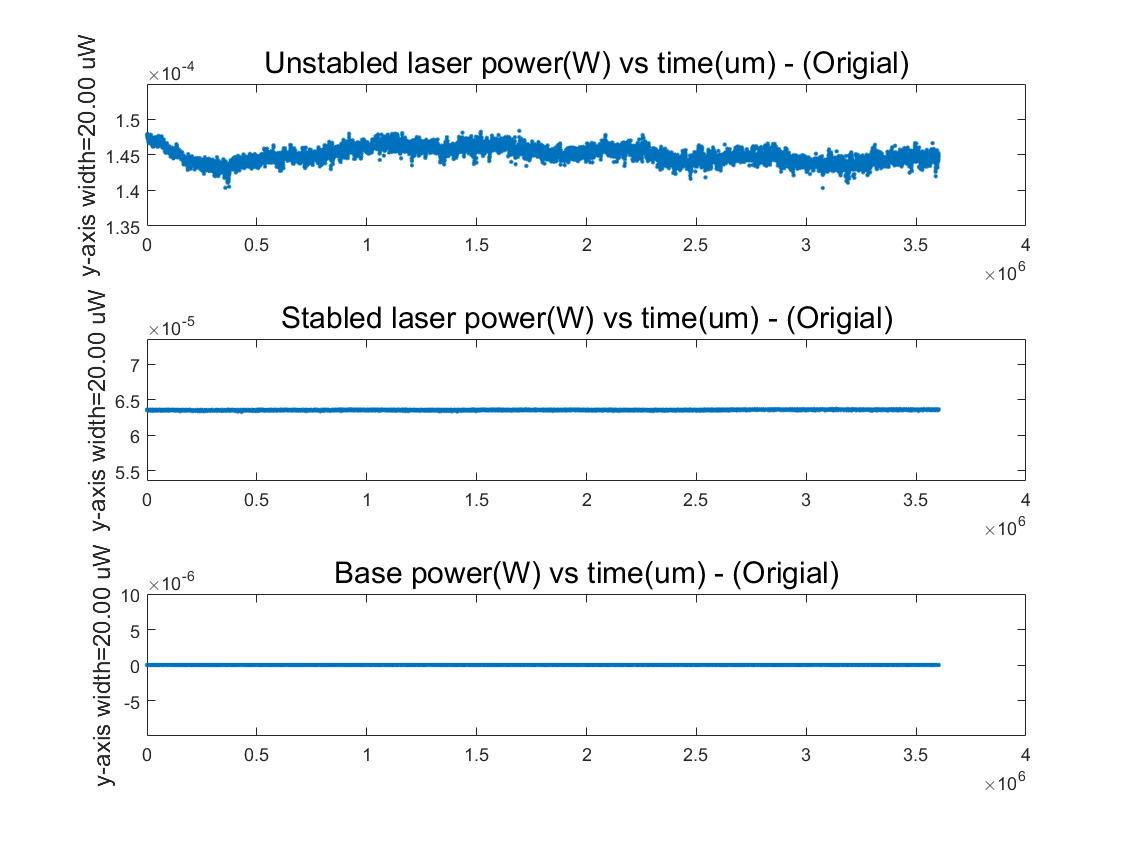
\includegraphics[width=0.8\linewidth]{laser_stabilization_data}
\end{figure}

\begin{figure}
    \centering
    \caption[激光功率外部稳定归一化后数据]{激光功率外部稳定归一化后本底、稳定前、稳定后数据。横坐标:时间(单位um),纵坐标:功率(单位uW)。\label{fig:laser_stabilization_data0}}
    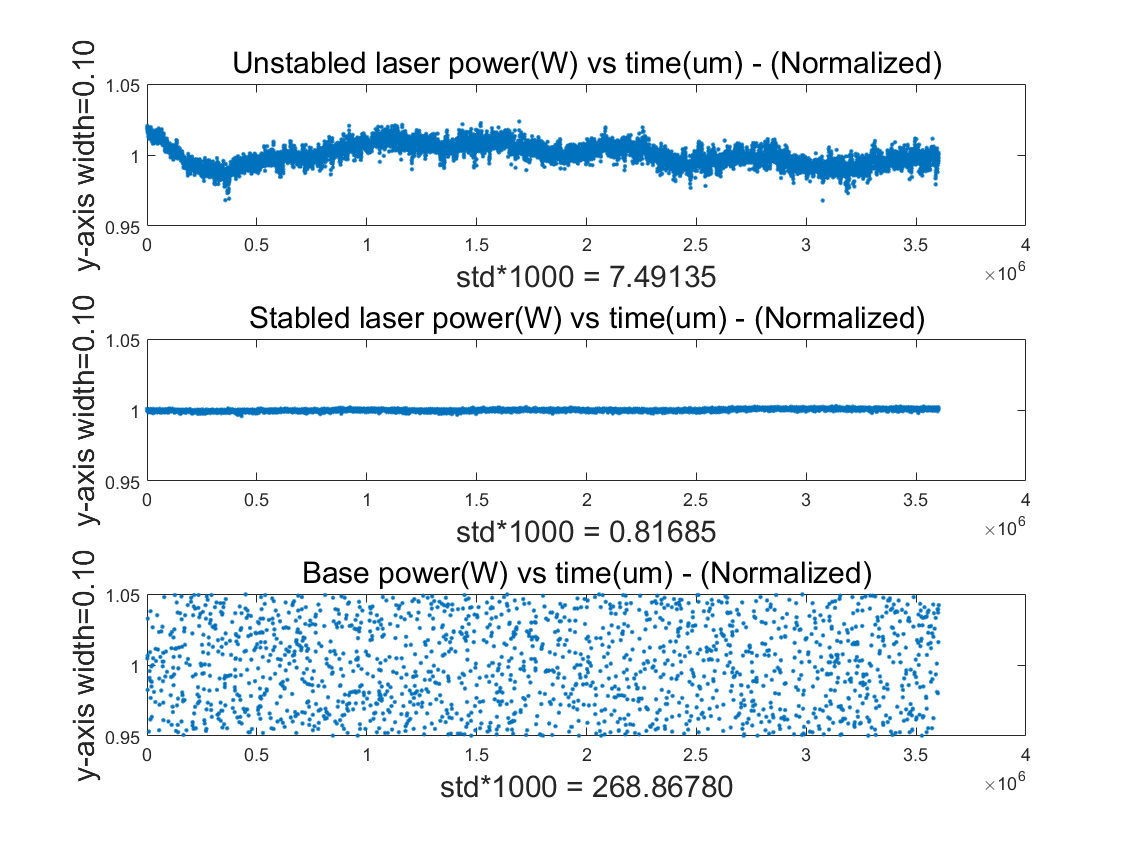
\includegraphics[width=0.8\linewidth]{laser_stabilization_data0}
\end{figure}


% 数据的测量采用如图所示的RIGOL DSG815示波器进行,在50kHz的采样率下采集约3.5s的数据。
为了能更好了解稳定效果的整体表现情况,我们以3Hz的采样率采集了激光功率稳定系统本底及稳定前后的数据。
激光功率外部稳定本底、稳定前、稳定后原始数据如图\ref{fig:laser_stabilization_data}所示,从图中看可以看出PD在无激光输入的暗态下本底噪声较小。除此之外,可以看到经过稳定后的激光功率小于稳定前的激光功率,这其中的主要原因是稳定过程中AOM动态分离了部分激光功率。为了能够有效地对比稳定前后的效果,我们用各组数据的均值对功率测试的结果进行归一化处理$P_{norm}=P_{original}/mean(P_{original})$,结果如图\ref{fig:laser_stabilization_data0}所示。由于本底噪声过于接近0,因此本底噪声的归一化结果呈现发散状态,在这里不具有参考价值。从图\ref{fig:laser_stabilization_data0}中可以明显看出经过数字PID稳定系统后的功率更加稳定了。
同时也绘制出了归一化后稳定前后数据的阿兰方差,如图\ref{fig:laser_stabilization_data2}所示,蓝色虚线为未稳定时的阿兰方差、橙色实线是稳定后的功率阿兰方差。从结果对比来看,稳定后的激光功率数据的阿兰方差在各个滑动窗口都低于未稳定时的,表明这里的数字稳定系统在较长时间的各个滑动窗口稳定性都好于未稳定时的,整体上有大约两个量级的改善。


\begin{figure}
    \centering
    \caption[激光功率外部稳定阿兰方差对比数据]{激光功率外部稳定归一化后本底、稳定前、稳定后数据阿兰方差。数据采样频率:3 Hz,横坐标:窗口长度(单位s),纵坐标:阿兰方差(单位1)。蓝色虚线为没有稳定情况下的功率阿兰方差,橙色实线是稳定后的功率阿兰方差。\label{fig:laser_stabilization_data2}}
    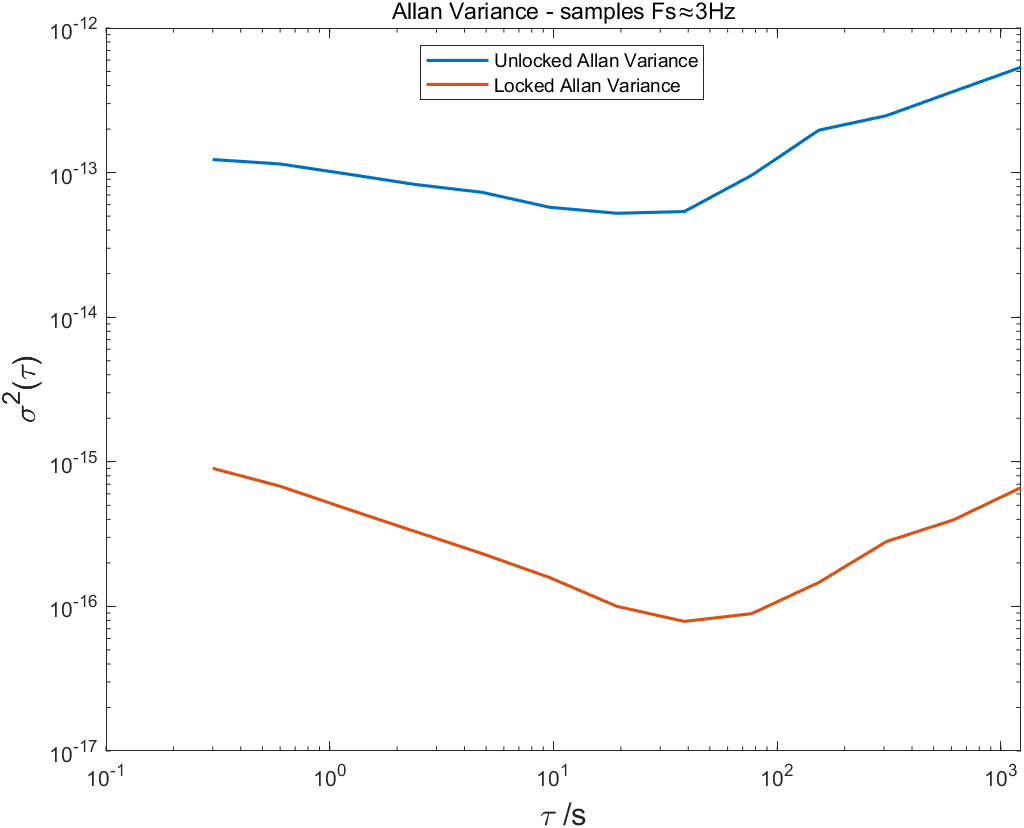
\includegraphics[width=0.8\linewidth]{laser_stabilization_data2}
\end{figure}

一般来说可以通过计算两组数据归一化后的方差之比可以粗略地获得稳定效果,方差越小稳定性越高。经计算稳定前后激光功率数据的方差比为$\frac{\sigma_{unstable}}{\sigma_{stabled}}\approx 9.17$。整体上经过激光功率稳定系统后,稳定前好了约9倍。为了能够更加直观地评估稳定的效果,我们将归一化后的所有数据点绘制出统计柱状图(由于本底的归一化不具有参考价值因此这里省略),结果如图\ref{fig:laser_stabilization_data1}所示。由公式\eqref{eq:amplitude_noise_fidelity}计算可知,激光幅度的相对标准差$\alpha$由$7.49135\times 10^{-3}$降低到$0.81685\times 10^{-3}$时,其对于角度翻转$\theta=\pi$的单量子比特操作保真度的影响可以由$1-99.9862\%$降低到$1-99.9998\%$,效果十分显著。


\begin{figure}
    \centering
    \caption[激光功率外部稳定柱状图对比数据]{激光功率外部稳定归一化后本底、稳定前、稳定后数据柱状图。横坐标:归一化后的激光功率数值(单位1),纵坐标:频数(单位1)。\label{fig:laser_stabilization_data1}}
    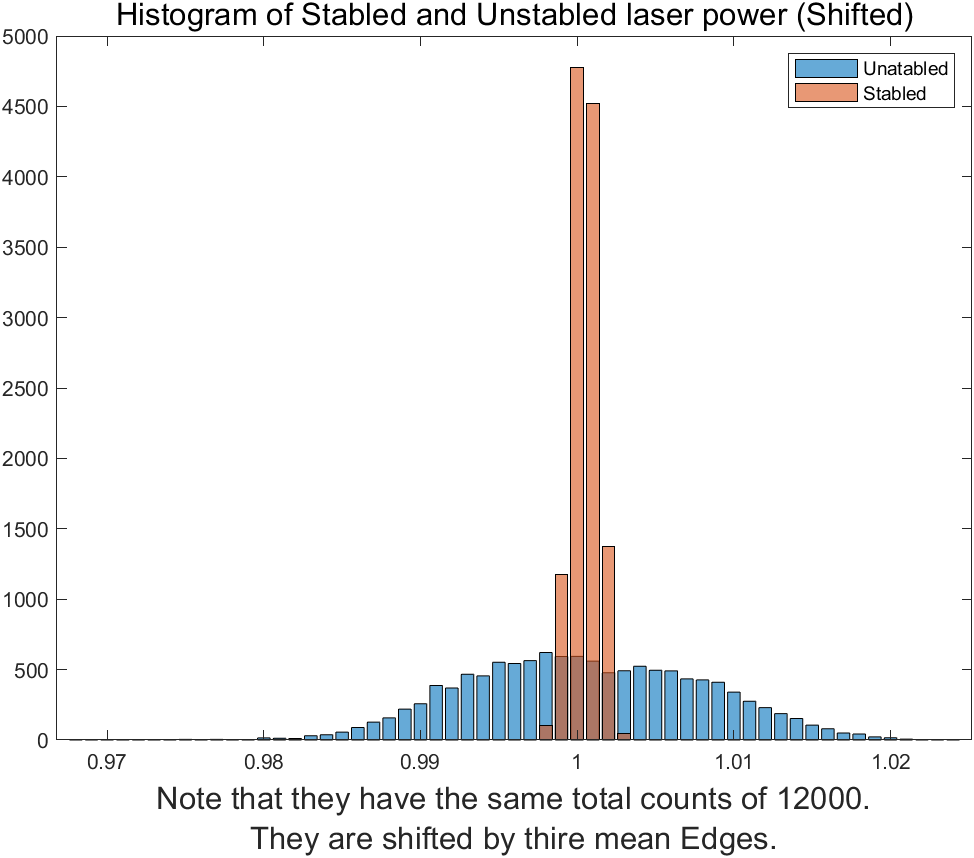
\includegraphics[width=0.8\linewidth]{laser_stabilization_data1}
\end{figure}












\newpage
\section[基于RTMQ的脉冲激光拍频稳定]{基于RTMQ的脉冲激光拍频稳定\label{section:pulsed_laser_locking}}
% ============================================================================
% ============================================================================
% =======================      激光拍频稳定     ===============================
% ============================================================================
% ============================================================================

量子信息通常会被编码在量子系统的不同能级结构中,比如第\ref{section:yb_computation}节中介绍的镱离子的内能级。这些能级能量差一般在微波或者光学波段,其量子比特状态通常可以用外部场操纵,例如微波或光场。在能级与外部场的耦合下,可以驱动量子状态发生改变,也即实现\emph{量子比特操控}。锁模(脉冲)激光器是可以实现此目的的通用仪器,其宽带光谱同时具有射频(RF)和微波结构。这种激光器已被用于控制原子\cite[]{Hayes_Matsukevich_Maunz_Hucul_Quraishi_Olmschenk_Campbell_Mizrahi_Senko_Monroe_2010}、分子\cite[]{Peer_Shapiro_Stowe_Shapiro_Ye_2007}和固态量子系统\cite[]{Greve_Press_McMahon_Yamamoto_2013}。
本节将首先介绍脉冲激光器及其拍频探测原理,接着给出基于RTMQ量子测控系统并结合前述通用数字PID和通用数字滤波器实现的一种简单技术来稳定脉冲激光的拍频,以便操作和控制通用量子比特系统\cite[]{ladd2010quantum}。
不同于之前常用的拍频锁定技术\cite[]{Islam_Campbell_Choi_Clark_Conover_Debnath_Edwards_Fields_Hayes_Hucul_et_al_2014},本方案通过使用板上集成的数字PID和数字滤波器,及大地提高了系统的稳定性和灵活性,并降低了实验的成本和空间的占用。


\subsection[脉冲激光器及其拍频探测原理]{脉冲激光器及其拍频探测原理}
\subsubsection[锁模(脉冲)激光器]{锁模(脉冲)激光器}
如第\ref{section:pulsed_laser_ion_operation}节中所述,锁模(脉冲)激光器可用于产生宽带光学频率梳,总带宽从$10$GHz到$100 $THz,梳齿由激光的重复速率$\omega_{rep}$间隔,通常在$0.1-1 $GHz范围内。量子比特的能级劈裂会匹配到重复频率的整数倍数附近,为了弥合与特定量子比特的频率差距,需要使用额外的光调制器完成微调\cite[]{Hayes_Matsukevich_Maunz_Hucul_Quraishi_Olmschenk_Campbell_Mizrahi_Senko_Monroe_2010}。为了在量子系统中保持长期相干性,与激光源相关的光学频率差必须稳定\cite[]{Stick_Hensinger_Olmschenk_Madsen_Schwab_Monroe_2006}。

产生稳定频率差的一种方便方法是将光源的光分成两条路径,将其中一束光进行微调,然后让它们在离子比特处交汇。这种方式可以避免激光共模波动引起的频率抖动问题\cite[]{Thomas_Hemmer_Ezekiel_Leiby_Picard_Willis_2002}。
一般来说,对于跃迁频率$\nu_{ab}\leq 1$GHz的情况,可以使用声光调制器(Acousto-Optic Modulator, AOM)产生相应的频率;对于高达$\nu_{ab} \sim 10 $GHz的较大跃迁频率,可以使用电光调制器(Electro-Optic Modulator, EOM),尽管由于频率调制边带会受到相位偏移模式影响被抑制\cite[]{Lee_Blinov_Brickman_Deslauriers_Madsen_Miller_Moehring_Stick_Monroe_2003}。锁模(脉冲)激光器可以产生不受此相位问题影响的调幅(AM)边带,成为生成调控边带的极佳方案。锁模(脉冲)激光器的带宽通常足够大,可以解决频率$\nu_{ab} < 100 $THz的能级劈裂。与AOM的适度频移相结合,可用于在该带宽内达到任意频率。

\subsubsection[脉冲激光的拍频探测原理]{脉冲激光的拍频探测原理}
对光频率的拍频探测是一个十分重要的环节,本质上对光频率的拍频探测就是对光能量的探测。对激光频率的拍频探测通常采用光电二极管组成的光探测器(Photon Detector, PD)。它的探测结果受到光电二极管的响应速度影响,比如响应速度小于1GHz的PD会过滤掉激光中超过1GHz的高频成分。我们的目标频率是光拍频结果中与离子比特能级共振的频率,即12.56GHz附近的频率。因此系统的搭建需要使用超快光探测器。接下来将具体介绍对脉冲激光的拍频探测原理。

脉冲激光的一般时域表示,考虑脉冲激光是幅度调制的连续激光:
\begin{align}
    E(t)=E_0 (t) e^{-i\omega_0 t}
\end{align}

从傅里叶分析角度表述:
\begin{align}
    E(t)=\left(\sum_{n=-\infty}^{\infty}\left[E_n e^{-in\omega_{rep}t} e^{-i\omega_0 t} \right]\right)\cdot e^{ikx}\cdot e^{i\phi}
\end{align}
其中$E_n$是频率为$n\omega_{rep}$的光频成分对应的电场大小,$k$是脉冲光的波矢,$\phi$是脉冲光的初始相位。
用超快光电探测器(Ultra-fast Photon Detector, UPD)探测一路脉冲光时得到光功率:
\begin{footnotesize}
\begin{align}
    P(t)=&|E(t)|^2=\left|\left(\sum_{n=-\infty}^{\infty}\left[E_n e^{-in\omega_{rep}t} e^{-i\omega_0 t} \right]\right)\cdot e^{ikx}\cdot e^{i\phi}\right|^2\\
    =&\left\{\left(\sum_{n=-\infty}^{\infty}\left[E_n e^{-in\omega_{rep}t} e^{-iω_0 t} \right]\right)\cdot e^{ikx}\cdot e^{i\phi}\right\} \cdot\left\{\left(\sum_{m=-\infty}^{\infty}\left[E^*_m e^{im\omega_{rep}t} e^{i\omega_0 t} \right]\right)\cdot e^{-ikx}\cdot e^{-i\phi}\right\}\\
    =&\sum_{n,m=-\infty}^{\infty}E_n e^{-in\omega_{rep} t} e^{-i\omega_0 t}\cdot E_m^* e^{im\omega_{rep} t} e^{i\omega_0 t}\\
    =&\sum_{n,m=-\infty}^{infty}E_n E_m^* e^{-i(n-m) \omega_{rep} t}\label{eq:pt_res1}
\end{align}    
\end{footnotesize}

针对公式\eqref{eq:pt_res1}分别考虑$n,m$的几类可能情况,原方程可化为:
\begin{footnotesize}
\begin{align}
    P(t)=&\sum_{n=m=-\infty}^{\infty}E_n E_m^*
    +\sum_{n>m=-\infty}^{\infty}E_n E_m^*e^{-i(n-m)\omega_{rep}t}+\sum_{n<m=-\infty}^{\infty}E_n E_m^*e^{-i(n-m)\omega_{rep}t}\\
    =&\sum_{n=m=-\infty}^{\infty}E_n E_m^*
    +\sum_{n>m=-\infty}^{\infty}E_n E_m^*e^{-i(n-m)\omega_{rep}t}+\sum_{m<m=-\infty}^{\infty}E_m E_n^*e^{-i(m-n)\omega_{rep}t}\\
    =&\sum_{n=m=-\infty}^{\infty}E_n E_m^*+\sum_{n>m=-\infty}^{\infty}E_n E_m^*e^{-i(n-m)\omega_{rep}t}+E_mE_n^* e^{i(n-m)\omega_{rep}t}
\end{align}
\end{footnotesize}

考虑电场强度为实数的情况下,可得:
\begin{align}
    P(t)=&\sum_{n=m=-\infty}^{\infty}E_n^2 + \sum_{n>m=-\infty}^{\infty}E_n E_m\left(e^{-i(n-m)\omega_{rep}t}+e^{i(n-m)\omega_{rep}t}\right)\\
    =&\sum_{n=m=-\infty}^{\infty}E_n^2 + \sum_{n>m=-\infty}^{\infty}E_n E_m\left(2\cos\left((n-m)\omega_{rep}t\right)\right)\\
    =&\sum_{n=m=-\infty}^{\infty}E_n^2 + \sum_{n>m=-\infty}^{\infty}2E_n E_m \cos\left((n-m)\omega_{rep}t\right)\label{eq:pt_res2}
\end{align}

这其中第一项为与时间无关项,反映到探测结果中就是UPD的直流成分;第二项是一些列的三角函数波,它们幅度相等,并具有$\omega_{rep}$的频率间隔,这便是单路脉冲光探测结果中的频率梳成分。

我们的方案是采用两路光同时作用在离子上的,下面讨论同时探测两路光得到的结果。假设两路光分别是$E_1(t),\ E_2(t)$,它们的探测结果为:
\begin{footnotesize}
\begin{align}
    P(t)=&\left|\left(\sum_{n_1=-\infty}^{\infty}E_{n_1}e^{-in_1\omega_{rep1}t}e^{-i\omega_{01}t}\right)\cdot e^{ik_1x}\cdot e^{i\phi_1} + \left(\sum_{n_2=-\infty}^{\infty}E_{n_2}e^{-in_2\omega_{rep2}t}e^{-i\omega_{02}t}\right)\cdot e^{ik_2x}\cdot e^{i\phi_2}\right|^2\\
    =&\left\{\left(\sum_{n_1=-\infty}^{\infty}E_{n_1}e^{-in_1\omega_{rep1}t}e^{-i\omega_{01}t}\right)\cdot e^{ik_1x}\cdot e^{i\phi_1} + \left(\sum_{n_2=-\infty}^{\infty}E_{n_2}e^{-in_2\omega_{rep2}t}e^{-i\omega_{02}t}\right)\cdot e^{ik_2x}\cdot e^{i\phi_2}\right\}\\
    +&\left\{\left(\sum_{m_1=-\infty}^{\infty}E_{m_1}^* e^{im_1\omega_{rep1}t}e^{i\omega_{01}t}\right)\cdot e^{-ik_1x}\cdot e^{-i\phi_1} + \left(\sum_{m_2=-\infty}^{\infty}E_{m_2}^*e^{im_2\omega_{rep2}t}e^{i\omega_{02}t}\right)\cdot e^{-ik_2x}\cdot e^{-i\phi_2}\right\}\label{eq:pt_res3}
\end{align}
\end{footnotesize}


公式\eqref{eq:pt_res3}的乘积展开有四项,分别为:
\begin{footnotesize}
\begin{align}
    P(t)=&RES1+RES2+RES3+RES4\\
    RES1=P_{1to1}(t)=&\left(\sum_{n_1=-\infty}^{\infty}E_{n_1}e^{-in_1\omega_{rep1}t}e^{-i\omega_{01}t}\right)\cdot e^{ik_1x}\cdot e^{i\phi_1} 
    \cdot \left(\sum_{m_1=-\infty}^{\infty}E_{m_1}^* e^{im_1\omega_{rep1}t}e^{i\omega_{01}t}\right)\cdot e^{-ik_1x}\cdot e^{-i\phi_1}\\
    RES2=P_{1to2}(t)=&\left(\sum_{n_1=-\infty}^{\infty}E_{n_1}e^{-in_1\omega_{rep1}t}e^{-i\omega_{01}t}\right)\cdot e^{ik_1x}\cdot e^{i\phi_1} 
    \cdot \left(\sum_{m_2=-\infty}^{\infty}E_{m_2}^*e^{im_2\omega_{rep2}t}e^{i\omega_{02}t}\right)\cdot e^{-ik_2x}\cdot e^{-i\phi_2}\\
    RES3=P_{2to1}(t)=&\left(\sum_{n_2=-\infty}^{\infty}E_{n_2}e^{-in_2\omega_{rep2}t}e^{-i\omega_{02}t}\right)\cdot e^{ik_2x}\cdot e^{i\phi_2}
    \cdot \left(\sum_{m_1=-\infty}^{\infty}E_{m_1}^* e^{im_1\omega_{rep1}t}e^{i\omega_{01}t}\right)\cdot e^{-ik_1x}\cdot e^{-i\phi_1}\\
    RES4=P_{2to2}(t)=&\left(\sum_{n_2=-\infty}^{\infty}E_{n_2}e^{-in_2\omega_{rep2}t}e^{-i\omega_{02}t}\right)\cdot e^{ik_2x}\cdot e^{i\phi_2}
    \cdot \left(\sum_{m_2=-\infty}^{\infty}E_{m_2}^*e^{im_2\omega_{rep2}t}e^{i\omega_{02}t}\right)\cdot e^{-ik_2x}\cdot e^{-i\phi_2}
\end{align}
\end{footnotesize}

其中RES1和RES4是单路脉冲光自相互作用的结果项,RES2和RES3是两路单路脉冲相互作用的结果项。RES1和RES4这种单路脉冲光自相互作用的探测结果前面公式\eqref{eq:pt_res2}已经讨论过了,结果可以直接类似写出如下:

\begin{align}
    RES1=P_{1to1}(t)=&\sum_{n_1=m_1=-\infty}^{\infty}E_{n_1}^2 + \sum_{n_1>m_1=-\infty}^{\infty}2E_{n_1} E_{m_1} \cos\left((n_1-m_1)\omega_{rep1}t\right)\label{eq:final_res1}\\
    RES4=P_{2to2}(t)=&\sum_{n_2=m_2=-\infty}^{\infty}E_{n_2}^2 + \sum_{n_2>m_2=-\infty}^{\infty}2E_{n_2} E_{m_2} \cos\left((n_2-m_2)\omega_{rep2}t\right)\label{eq:final_res4}
\end{align}


下面重点讨论RES2和RES3这类两路光相互作用的项。
\begin{footnotesize}
\begin{align}
    RES2=P_{1to2}(t)=&\left(\sum_{n_1=-\infty}^{\infty}E_{n_1}e^{-in_1\omega_{rep1}t}e^{-i\omega_{01}t}\right)\cdot e^{ik_1x}\cdot e^{i\phi_1} 
    \cdot \left(\sum_{m_2=-\infty}^{\infty}E_{m_2}^*e^{im_2\omega_{rep2}t}e^{i\omega_{02}t}\right)\cdot e^{-ik_2x}\cdot e^{-i\phi_2}\\
    =&\sum_{n_1,m_1=-\infty}^{\infty}E_{n_1}E_{m_2}^*e_1^{-i(n_1\omega_{rep1}-m_2\omega_{rep2})t}e^{-i(\omega_{01}-\omega_{02})t}e^{i(k_1-k_2)x}e^{i(\phi_1-\phi_2)}
\end{align}
\end{footnotesize}

此时考虑具体情况,这两束光为同一束脉冲光中分出的,则有$E_{n_2}=kE_{n_1}$,$\omega_{rep1}=\omega_{rep2}$,此时上面结果变为:
\begin{footnotesize}
\begin{align}
    RES2=P_{1to2}(t)=&\sum_{n_1,m_1=-\infty}^{\infty}E_{n_1}kE_{m_2}^*e_1^{-i(n_1-m_2)\omega_{rep1}t}e^{-i(\omega_{01}-\omega_{02})t}e^{i(k_1-k_2)x}e^{i(\phi_1-\phi_2)}
\end{align}
\end{footnotesize}

前面计算过电场为实数时的情况,类似的可以得到:
\begin{align}
    \sum_{n,m=-\infty}^{\infty}E_nE_m^*e^{-i(n-m)\omega_{rep}t}=\sum_{n=m=-\infty}^{\infty}E_n^2+\sum_{n>m=-\infty}^{\infty}2E_nE_m\cos((n-m)\omega_{rep}t)
\end{align}

此时,记e指数项相关的变量$\Delta\omega=\omega_{01}-\omega_{02},\ \Delta k=k_1-k_2,\ \Delta\phi=\phi_1-\phi_2$,RES2结果变为:
\begin{footnotesize}
\begin{align}
    RES2=P_{1to2}(t)=&\left\{\sum_{n_1=m_2=-\infty}^{\infty}kE_{n_1}^2+\sum_{n_1>m_2=-\infty}^{\infty}2E_{n_1}E_{m_2}(e^{-i(n_1-m_2)\omega_{rep1}t}+e^{i(n_1-m_2)\omega_{rep1}t})\right\}\\
    & \cdot e^{-i(\Delta\omega)t}e^{i(\Delta k)x}e^{i\Delta\phi}\\
    =&\left\{\sum_{n_1=m_2=-\infty}^{\infty}kE_{n_1}^2+\sum_{n_1>m_2=-\infty}^{\infty}2E_{n_1}E_{m_2}\cos((n_1-m_2)\omega_{rep}t)\right\}\notag\\
    & \cdot (\cos\Delta\omega t-i\sin\Delta\omega t)e^{i(\Delta k)x}e^{i\Delta\phi}\label{eq:final_res2}
\end{align}
\end{footnotesize}

同理,RES3的计算可以相应地得到。若记$\Delta\omega=\omega_{02}-\omega_{01},\ \Delta k=k_2-k_1,\ \Delta\phi=\phi_2-\phi_1$,则RES2最后的结果与公式\eqref{eq:final_res2}类似,结果如下:
\begin{small}
\begin{align}
    RES3=P_{2to1}(t)=&\left\{\sum_{n_1=m_2=-\infty}^{\infty}kE_{n_1}^2+\sum_{n_1>m_2=-\infty}^{\infty}2E_{n_1}E_{m_2}\cos((n_1-m_2)\omega_{rep}t)\right\}\notag\\
    & \cdot (\cos\Delta\omega t+i\sin\Delta\omega t)e^{-i(\Delta k)x}e^{-i\Delta\phi}\label{eq:final_res3}
\end{align}    
\end{small}

最后,两路来自同一脉冲束的光作用的探测结果$P(t)$可以由公式\eqref{eq:final_res1}公式\eqref{eq:final_res2}公式\eqref{eq:final_res3}公式\eqref{eq:final_res4}结果共同写出:
\begin{small}
\begin{align}
    P(t)=&\sum_{i=1}^{4}RES_i\\
    =&\sum_{n_1=m_1=-\infty}^{\infty}E_{n_1}^2 + \sum_{n_1>m_1=-\infty}^{\infty}2E_{n_1} E_{m_1} \cos\left((n_1-m_1)\omega_{rep1}t\right)\\
    &+\left\{\sum_{n_1=m_2=-\infty}^{\infty}kE_{n_1}^2+\sum_{n_1>m_2=-\infty}^{\infty}2E_{n_1}E_{m_2}\cos((n_1-m_2)\omega_{rep}t)\right\}\notag\\
    & \cdot (\cos\Delta\omega t-i\sin\Delta\omega t)e^{i(\Delta k)x}e^{i\Delta\phi}\\
    &+\left\{\sum_{n_1=m_2=-\infty}^{\infty}kE_{n_1}^2+\sum_{n_1>m_2=-\infty}^{\infty}2E_{n_1}E_{m_2}\cos((n_1-m_2)\omega_{rep}t)\right\}\notag\\
    & \cdot (\cos\Delta\omega t+i\sin\Delta\omega t)e^{-i(\Delta k)x}e^{-i\Delta\phi}\\
    &+\sum_{n_2=m_2=-\infty}^{\infty}E_{n_2}^2 + \sum_{n_2>m_2=-\infty}^{\infty}2E_{n_2} E_{m_2} \cos\left((n_2-m_2)\omega_{rep2}t\right)
\end{align}
\end{small}

经一步化简得到,两路来自同一脉冲束的光作用的探测结果$P(t)$表达式为:
% \begin{small}
\begin{align}
    P(t)=&\sum_{n_1=m_1=-\infty}^{\infty}(k^2+1)E_{n_1}^2\label{eq:pulsed_01}\\
    &+\sum_{n_1>m_1=-\infty}^{\infty}2(k^2+1)E_{n_1}E_{m_1}\cos\left((n_1-m_1)\omega_{rep}t\right)\label{eq:pulsed_02}\\
    &+\sum_{n_1=m_1=-\infty}^{\infty}2kE_{n_1}^2\cos\Delta\omega t\label{eq:pulsed_03}\\
    &+\sum_{n_1>m_1=-\infty}^{\infty}2kE_{n_1}E_{m_1}\cos\left((n_1-m_1)\omega_{rep}t\right)cos\Delta\omega t\label{eq:pulsed_04}
\end{align}
% \end{small}

这其中第一项\eqref{eq:pulsed_01}贡献了探测结果中的直流项;第二项\eqref{eq:pulsed_02}贡献了结果中的间隔频率为$\omega_{rep}$的频率梳齿项;第三项\eqref{eq:pulsed_03}贡献了频率为调制频率差$\Delta\omega$的项;第四项\eqref{eq:pulsed_04}贡献了各个频率梳齿两侧相距中心梳齿$\Delta\omega$的边带项。第四项的频率梳齿边带正是要稳定的目标频率项,里面包含了外部可调节项$\Delta\omega$,而这一项来可以是AOM。我们可以通过设计控制回路,通过AOM输出控制信号$\Delta\omega$,进而使得目标频率$(n_1-m_1)\omega_{rep}\pm \Delta\omega$稳定在量子比特编码能级频率差$\nu_{qubit}$上。

\subsection[基于RTMQ系统的激光拍频稳定原理]{基于RTMQ系统的激光拍频稳定原理}

如图\ref{fig:beat_note_stabilization}所示,为了调整驱动量子比特跃迁的场的频率,来自锁模(脉冲)激光器的光束被分成两条路径,在各自支路上分别受到$\nu_{M1}$和$\nu_{M2}$的频率调制,然后在离子比特上重新交汇。
两条光路尽量等长(不必须严格等长或在光学波长尺度上长期稳定),并需要微调光路长度以使得脉冲能在离子比特处交汇。

\begin{figure}
    \centering
    \caption[脉冲激光拍频稳定系统框图]{脉冲激光拍频稳定系统框图。AOM:声光调制器;PD:光功率探测器;DDS:数字频率生成器;PID:比例积分微分控制器;FOL:频率低通滤波器;ADC:模拟数字转化器。\label{fig:beat_note_stabilization}}
    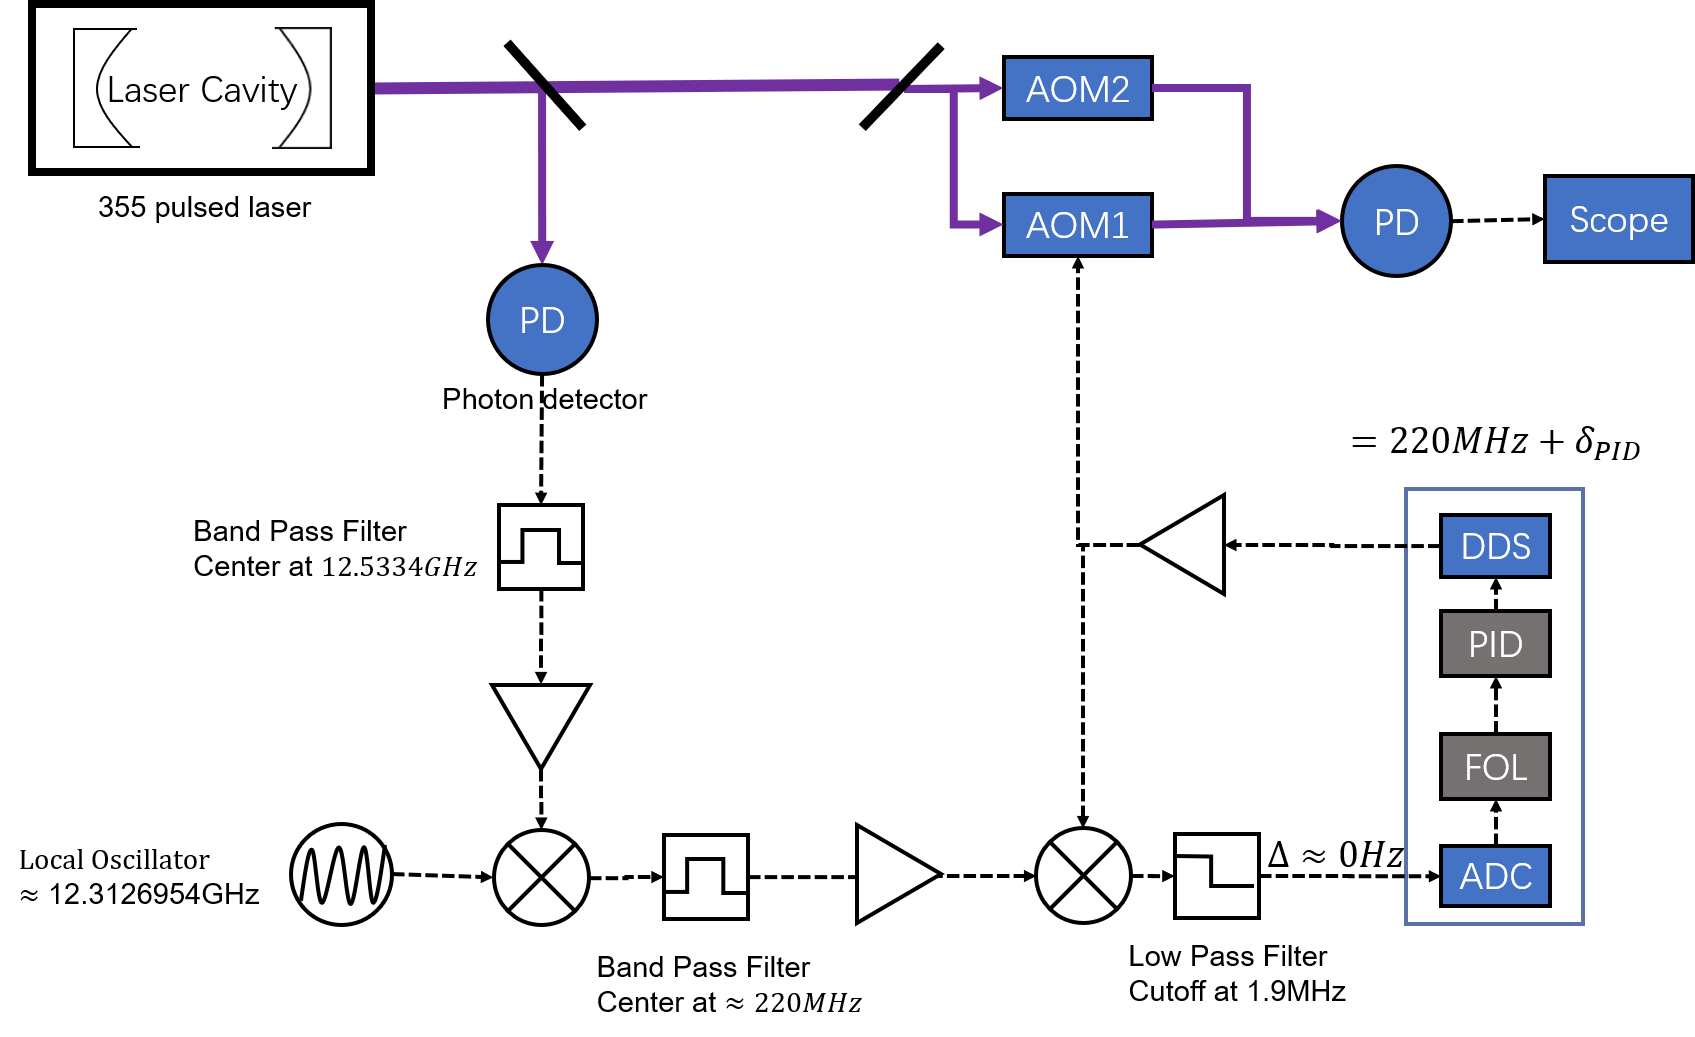
\includegraphics[width=1.0\linewidth]{beat_note_stabilization}
\end{figure}

图\ref{fig:frequency_comb}显示了由快速光电二极管测量的光束的结果RF光谱,由每个单独光束的激光重复率$\nu_{rep}$分隔,以及经AOM调制后组合光束的$\nu_{rep}\pm |\Delta \nu_M|$分隔的附加拍频边带,其中$|\Delta \nu_M|=|\nu_{M1}-\nu_{M2}|$。
我们通过调整路径$\Delta\nu_M$的相对频移来控制这些额外边带的位置,使之与编码量子信息的能级共振。经调制后用于调控离子的目标边带为$\nu_{sb}$,可以表达为:
\begin{align}
    \nu_{sb}=n\nu_{rep}\pm|\Delta\nu_M|
\end{align}

\begin{figure}
    \centering
    \caption[脉冲激光频率梳]{在频谱分析仪中看到的脉冲激光频率梳。激光频率梳由每个单独光束的激光重复率$\nu_{rep}$分隔,以及经AOM调制后组合光束的$\nu_{rep}\pm |\Delta \nu_M|$分隔的附加拍频边带,其中$|\Delta \nu_M|=|\nu_{M1}-\nu_{M2}|$。由于微波传输线、滤波器及网分自身频率特性等作用,观察到的频率梳并非理想形状。\label{fig:frequency_comb}}
    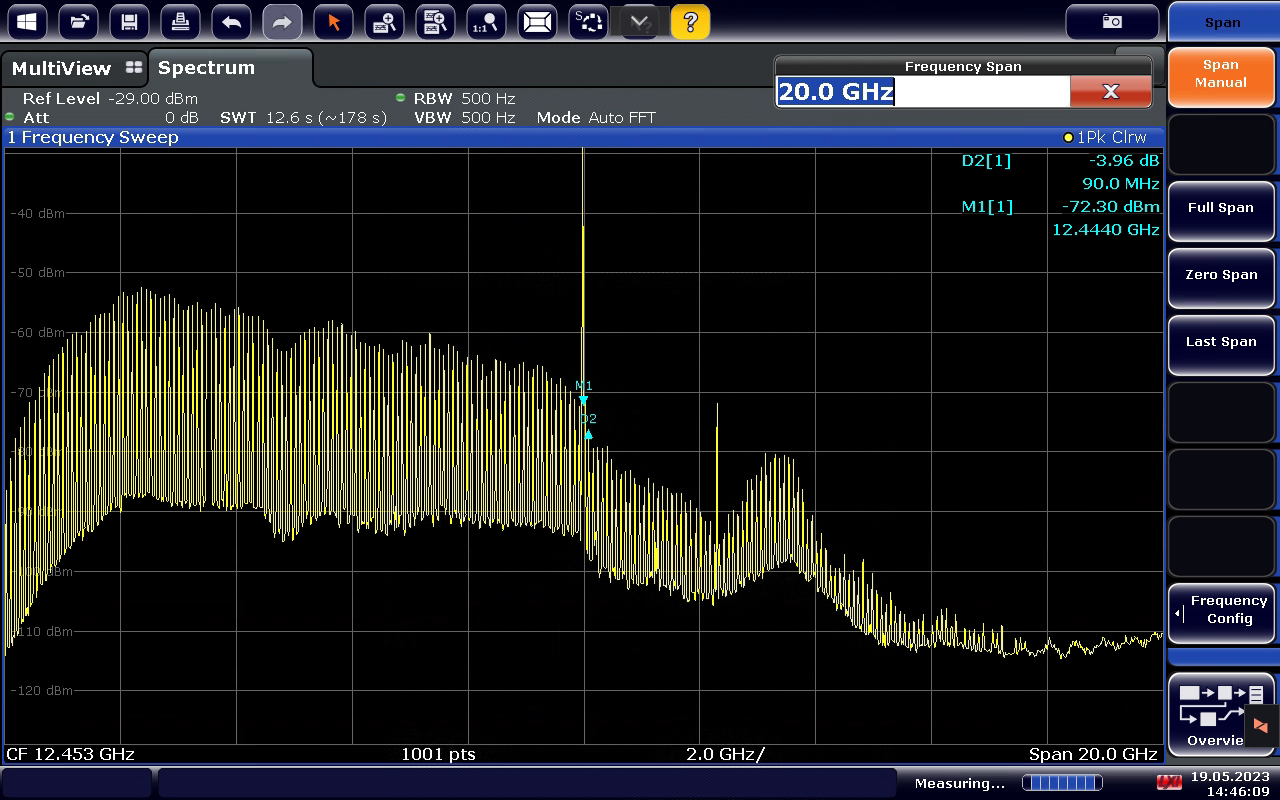
\includegraphics[width=0.8\linewidth]{frequency_comb}
\end{figure}

其中$n$是某个整数,$\nu_{sb}$在频率梳的带宽内。注意采用拉曼跃迁的方式操控时(第\ref{section:raman_transition}节),如图\ref{fig:raman_transition1}所示,激光载波包络相位不需要稳定\cite[]{Peer_Shapiro_Stowe_Shapiro_Ye_2007},尽管也有类似的方式可以完成\cite[]{Koke_Grebing_Frei_Anderson_Assion_Steinmeyer_2010}。

\begin{figure}
    \centering
    \caption[受激拉曼跃迁示意图]{受激拉曼跃迁示意图。$\ket{e}$:上级激发态能级;$\ket{a},\ket{b}$:编码量子信息的高低能级;$\nu_{ab}$:编码量子信息的能级能隙;$\nu_{a}$:$\ket{e}$能级与$\ket{b}$能级的能隙;$\nu_a^L$:$\ket{a}$能级与虚拟能级的能隙;$\nu_b^L$:$\ket{b}$能级与虚拟能级的能隙。\label{fig:raman_transition1}}
    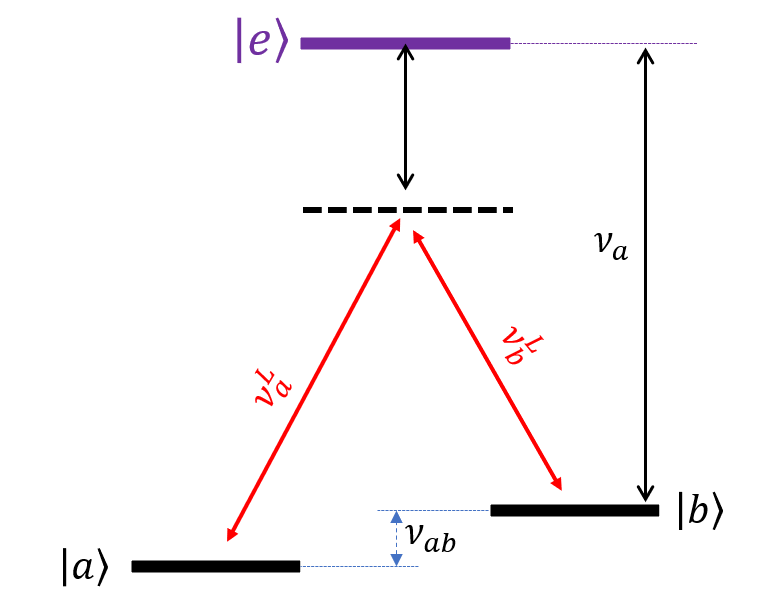
\includegraphics[width=0.6\linewidth]{raman_transition1}
\end{figure}

驱动量子比特需要梳齿之间的光学相干性在量子比特操作的毫秒或更快的时间尺度上保持,这对于锁模(脉冲)激光源来说很容易实现\cite[]{Hayes_Matsukevich_Maunz_Hucul_Quraishi_Olmschenk_Campbell_Mizrahi_Senko_Monroe_2010}。然而,由于激光腔长中的热应变或其它机械应变,激光重复频率会产生漂移[$\nu_{rep}=\nu_{rep}(t)$],导致施加的边带频率$\nu_{sb}$也跟着漂移,进一步地对量子比特驱动也将偏离共振。因此需要一定的措施来稳定用于操控量子比特的边带频率。

经典上采用将误差信号反馈给激光腔长的方式稳定重复率,不过当激光腔长不可调解时将无法实现。此外,这样的锁的带宽将有限,因为测量激光重复率的采集时间和使用机械换能器调制激光腔长度的延迟可能比激光腔波动的特征时间长。例如,$^{171}Yb$($12.642819 $GHz)电子基态的超精细跃迁在$ \nu_{rep} \sim 80.65$MHz处接近锁模频率激光器的第 157 梳齿。
想要将上述频率稳定在1kHz以内的话,一种经典的方法是测量$\nu_{rep}(t)$使其达到几赫兹的分辨率,而这需要的积分时间将超过1s\cite[]{Islam_Campbell_Choi_Clark_Conover_Debnath_Edwards_Fields_Hayes_Hucul_et_al_2014}。这种过于慢的稳定方式并不适合用来稳定频率梳齿的拍频边带。

作为替代,我们选择使用频率梳齿的$n\nu_{rep}(t)$与本地标准参考信号$\nu_{LO}$进行拍频的方式来检测频率的漂动。如图\ref{fig:beat_note_stabilization}所示,我们将锁模(脉冲)激光分出一部分与用FPD进行探测,然后经过一个12.5GHz为中心的带通滤波器并放大后,将其与在12.56GHz附近的本地振荡源拍频。两者拍频之后经过一个合适的低通或带通滤波器就可以获得一个差频信号$|n\nu_{rep}-\nu_{LO}|$(两者的绝对大小不重要,我们总是可以观测到正的差频)。接着将这个差频信号放大并与板卡的DDS输出频率进行拍频和滤波获得一个更小的差频信号,将这个信号送入板卡的ADC进行模数转换,随后经过数字滤波器和数字PID的处理对DDS的频率进行调节。整个控制器是采用数字系统实现的,主要涉及模块包括16位ADC(Linear Technology, LTC2216)、16位滤波器(第\ref{section:digital_iir}节)、16位PID(第\ref{section:digital_pid}节)、32位DDS(Analog Device, AD9910)。



\subsection[基于RTMQ的脉冲激光拍频稳定系统搭建及结果]{基于RTMQ的脉冲激光拍频稳定系统搭建及结果}


\begin{figure}
    \centering
    \caption[脉冲激光拍频稳定实验系统图]{脉冲激光拍频稳定实验系统图\label{fig:beat_note_stabilization_real}}
    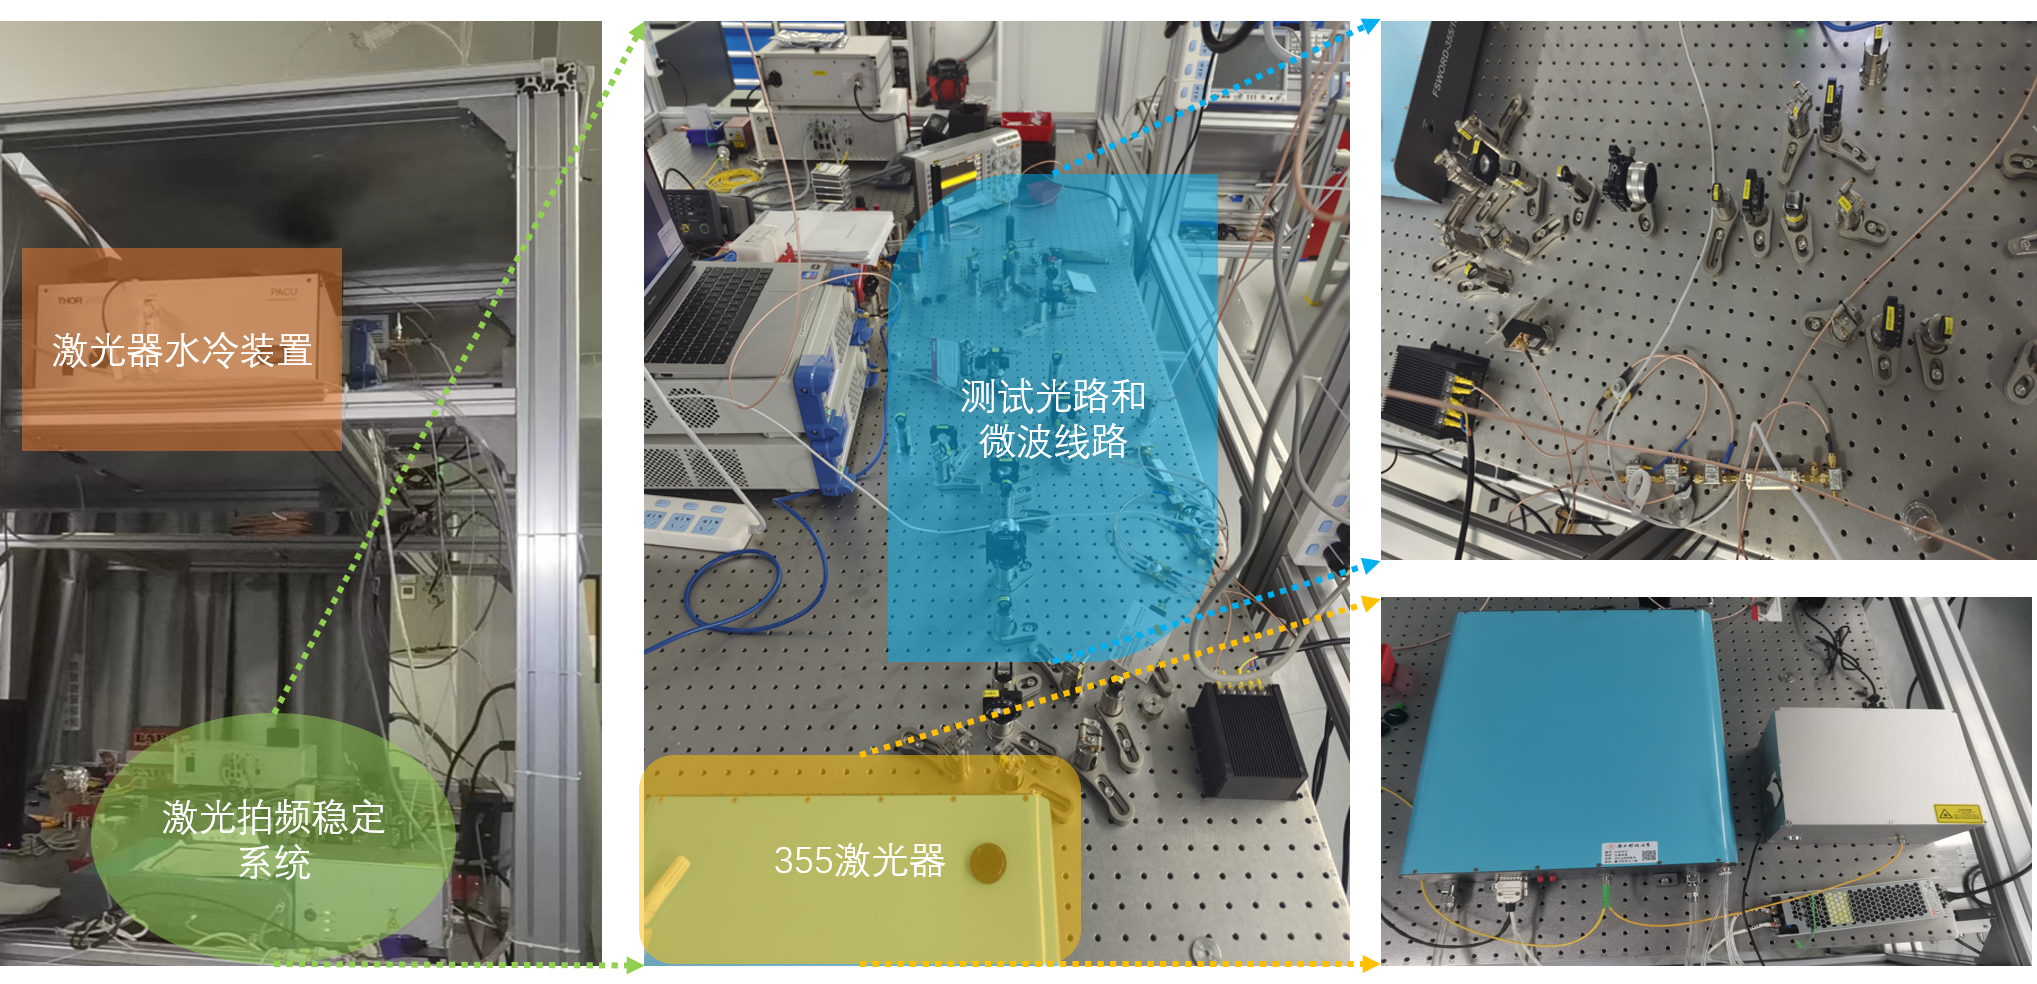
\includegraphics[width=1.0\linewidth]{beat_note_stabilization_real}
\end{figure}

脉冲激光拍频稳定系统实物如图\ref{fig:beat_note_stabilization_real}所示。激光拍频稳定的结果如图\ref{fig:beat_note_stabilization_signal}所示,图中展示了在12.39GHz附近的一个稳定的拍频边带。实验中可以利用此类似这样的稳定后的边带与离子进行相互作用,进而实现对离子量子比特的调控。值得一提的是,尽管系统稳定是针对某一级(例如157级)频率梳齿的边带进行稳定的,实际上整个频率梳齿的边带都会一定程度上被稳定下来。不过由于锁模(脉冲)激光重复频率的长期漂动,距离目标稳定边带越远的边带稳定效果越差。根据实验观测355脉冲激光在12.39GHz附近的拍频结果未稳定前标准差约为15kHz左右,稳定后的标准差约为100Hz左右,稳定性有了约150倍的提高。镱离子的典型拉比频率约为8.33MHz,结合公式\eqref{eq:frequency_noise_fidelity}计算可知,其对于角度翻转$\theta=\pi$的单量子比特操作保真度的影响从完全不能用的约$1-50\%$降低到了约$1-99.942\%$。

\begin{figure}
    \centering
    \caption[脉冲激光拍频稳定12.39GHz附近稳定边带结果]{脉冲激光拍频稳定12.39GHz附近稳定边带结果\label{fig:beat_note_stabilization_signal}}
    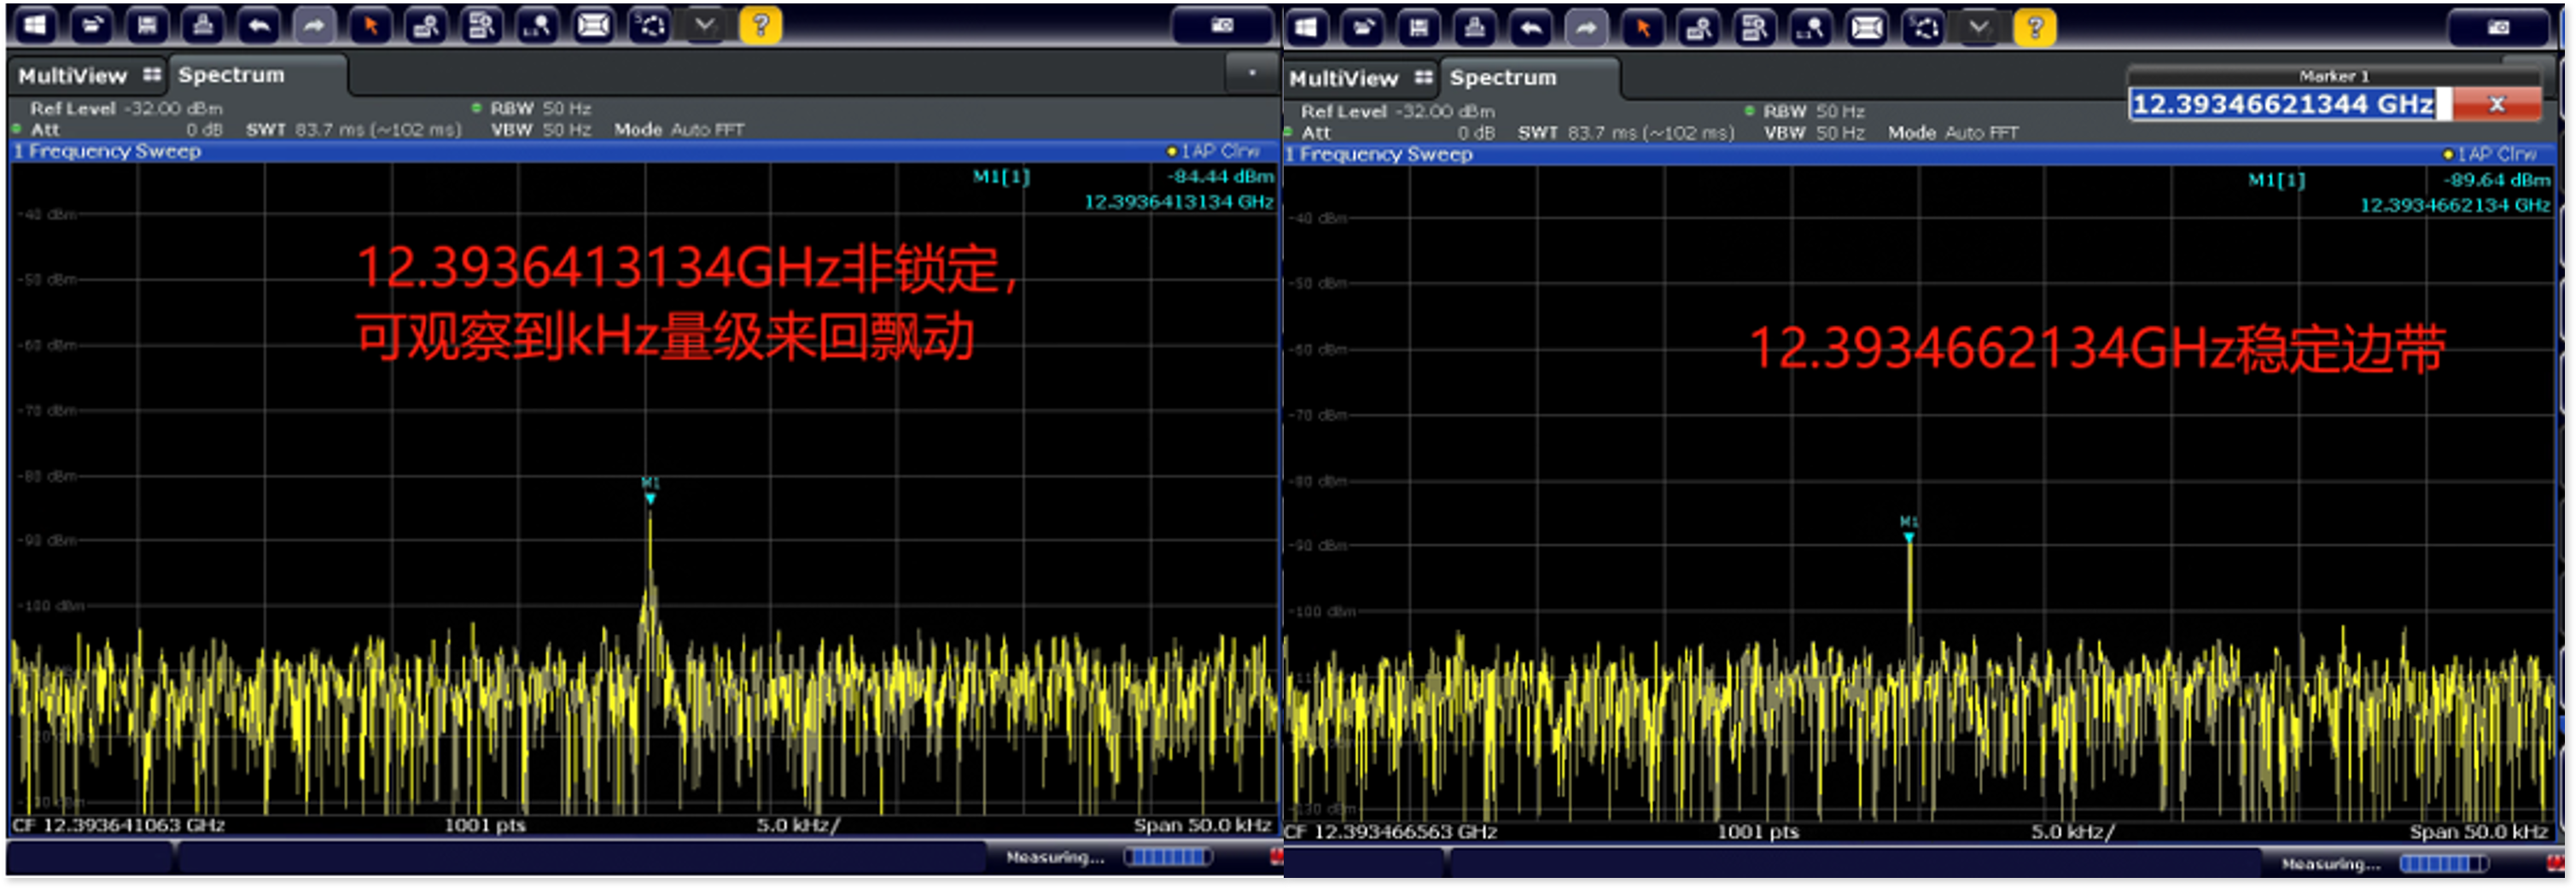
\includegraphics[width=1.0\linewidth]{beat_note_stabilization_signal}
\end{figure}

\subsubsection[拍频稳定系统的可锁频率幅度]{拍频稳定系统的可锁频率幅度}
由于锁模(脉冲)激光重复频率的长期漂动,数字PID拍频稳定系统需要对其进行补偿来使得频率符合预期值。然而拍频稳定系统并不能应付无限大的频率漂移。\emph{可锁频率幅度}表示了锁频系统对拍频结果的长期漂移的最大可接受范围,超过此范围的长期频率漂动将无法被稳定。下面讨论关于系统的可锁频率幅度相关问题。

该系统结合了大量数字系统,它的控制器和频率输出都由数字系统实现,这及大地提高了系统的稳定性和灵活性。控制器采用了数字PID,调节频率输出采用了DDS。因此理论上只要DDS的输出可以跟得上,应该能稳定接近DDS输出的可调节频率幅度。系统中采用的DDS的频率编码为32bit,频率范围为400MHz。寄存器的数值$R_{DDS}$和实际输出的模拟频率$f_{DDS}$的换算关系为:
\begin{align}
    f_{DDS}=\frac{R_{DDS}}{2^{32}}\times 400\ \textnormal{MHz}
\end{align}

DDS数字对应的\emph{频率步长}为$f_{resolution}=\frac{400\textnormal{MHz}}{2^{32}}\approx0.093\textnormal{Hz}$。然而,DDS芯片中给出的并行频率调制位数是16位,而实际的频率分辨率是32位,这意味着没有办法并行进行全部(0-400MHz)范围内的频率调制。
实际的使用中可以设定一个中心频率$f_{c}$,然后通过16位并行调制字再对这个频率进行微调$\Delta f$。另外,这16位并行调制字可以通过移位$N_{shift}$来对应的32位频率调制字的不同位数,以获得不同的调节范围。每左移一位,并行调制字的权重乘2,最大可移位数为15。也即,16位频率调制字的调制效果$\Delta f$为:
\begin{align}
    \Delta f=f_{resolution}\times n \times 2^{N_{shift}}
\end{align}

其中$n$是16位频率调制字对应的十进制无符号数。最终,DDS的并行调制频率结果为:
\begin{align}
    f_{dds}=f_c+f_{resolution}\times n \times 2^{N_{shift}}
\end{align}

\begin{figure}
    \centering
    \caption[频率调制字位移数vs调制精度
    ]{频率调制字位移数vs调制精度。频率调制字位移数与调制精度两者满足关系$f_{precision}=f_{resolution}\times2^{N_{shift}}$。
    \label{fig:beat_note_resolution_shift}}
    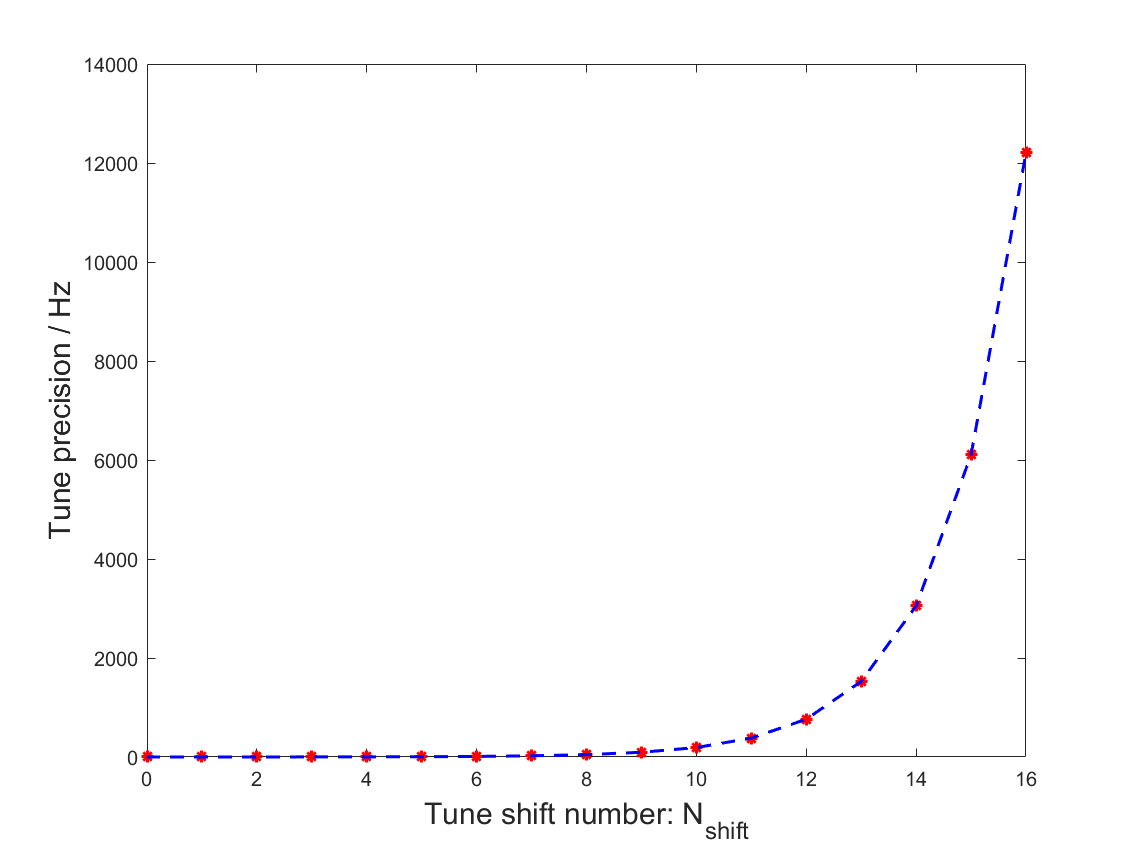
\includegraphics[width=0.8\linewidth]{beat_note_resolution_shift}
\end{figure}

需要注意的是在每次的位移后,并行调制的调制频率步长也会增加2倍,也即频率分辨率会相应下降2倍。频率调制字位移数与调制步长的关系如图\ref{fig:beat_note_resolution_shift}所示,频率调制字位移数与调制精度两者满足关系$f_{precision}=f_{resolution}\times2^{N_{shift}}$。



\begin{figure}
    \centering
    \caption[脉冲激光拍频稳定可锁频率幅度测试]{脉冲激光拍频稳定可锁频率幅度测试。蓝色虚线给出了前7个数据点关于公式$f(x)=a\times e^{b\times x}+c$的拟合结果,结果为:a=21.54,95\%置信区间(4.323,38.76);b=0.7487 ,95\%置信区间(0.5666,0.9308);c=-18.03,95\%置信区间(-56.06,20)。\label{fig:beat_note_lockable_range_bits}}
    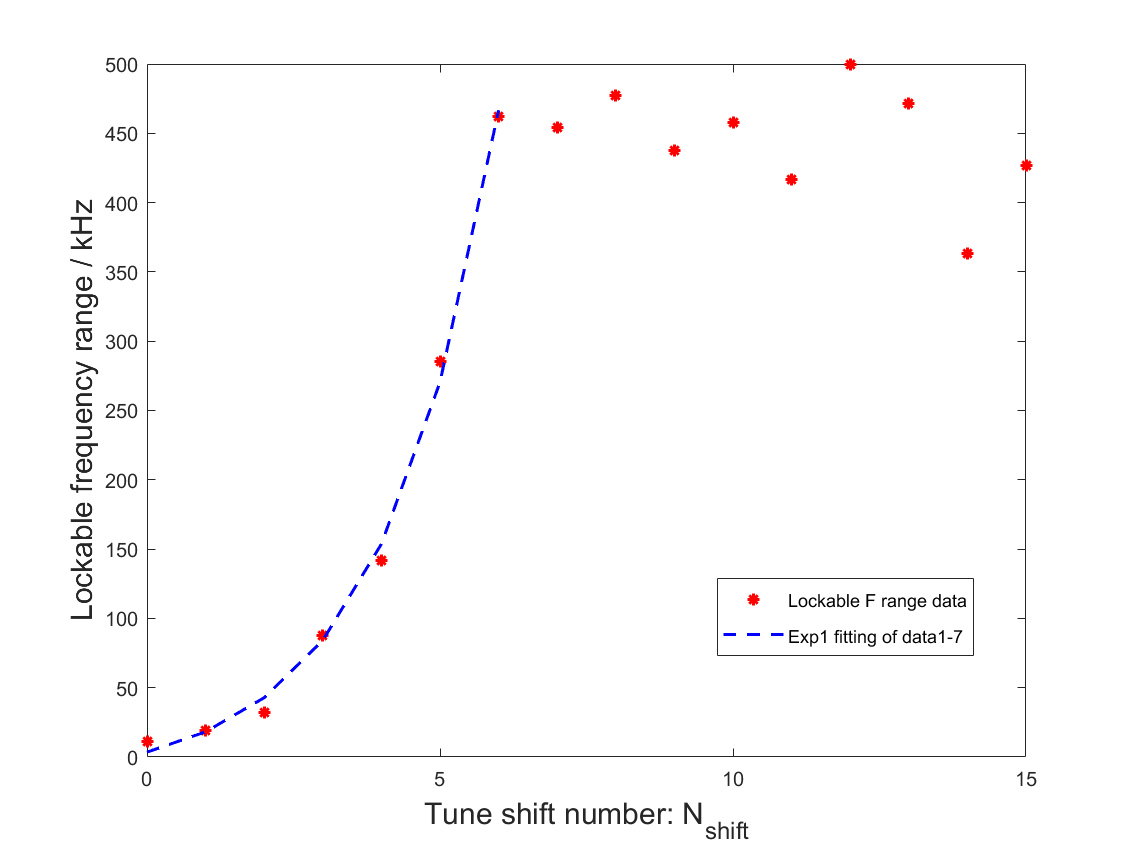
\includegraphics[width=0.8\linewidth]{beat_note_lockable_range_bits}
\end{figure}

通过计算可知,当16位并行调制字移位为0时,可以调节的频率范围仅为约6kHz。在数字PID和DDS的连接一定的情况下,为了测试整个拍频稳定系统的最大可锁频率幅度,可以通过不断移位并行调制字,来测得整个锁频系统最大的可锁频率幅度。测量结果如图\ref{fig:beat_note_lockable_range_bits}所示,理论上在移位到15之前每次移位后测的的可锁频率幅度相对前一种情况应该乘2。图中蓝色虚线给出了前7个数据点关于公式$f(x)=a\times e^{b\times x}+c$的拟合结果,结果为:a=21.54,95\%置信区间(4.323,38.76);b=0.7487 ,95\%置信区间(0.5666,0.9308);c=-18.03,95\%置信区间(-56.06,20)。

从图\ref{fig:beat_note_lockable_range_bits}中可见在移位0-6之间时基本符合可锁频率幅度岁位移数依次增大2倍这个规律,而到6之后可锁频率幅度便基本保持稳定了。从中可以得出在当前配置下,整个系统的最大可锁频率幅度约为450kHz。这个数值的限制因素主要可能有两个原因:1. 频率调制分辨率过低,导致无法稳定到目标频率上;2. 数字PID带宽影响;3. 系统中存在限制带宽的器件。联系到为了提升调制品质和减少噪声影响,我们的数字系统在PID前添加了一个数字低通滤波器,它的带宽约为450kHz。因此该数字低通滤波器应该是这个结果的主要影响因素。不过由于450kHz的可锁频率范围完全够用了,可以不用再这方面进行进一步优化。如果需要更宽的可锁频率范围,可以通过重新设计该数字低通滤波器的形状和带宽来方便地实现。








\newpage
\section[章末小结]{章末小结}

离子阱量子计算系统是一个涉及多种学科领域的复杂综合系统,离子囚禁、射频和激光在其中占据着至关重要的地位。本章介绍了经典信号对量子操作保真度的影响,给出了一套基于RTMQ架构的测控板硬件设计及其一些重要外设拓展固件的FPGA实现,展示了基于RTMQ量子测控系统实现的离子阱频率稳定、激光功率稳定以及激光拍频稳定等几个离子阱量子计算的关键子系统以提高量子比特操作的保真度。

使用RTMQ架构的测控板硬件设计选用了Xilinx的Artix-7系列功能最强大的FPGA芯片,并且针对离子阱量子计算实验中常用的功能集成了相应的芯片,如ADC模数转换芯片、DAC数模转换芯片、DDS数字频率生成器芯片等,同时采用了专门的时钟管理芯片为系统各功能模块提供统一的时钟管理。该测控板硬件设计能够满足RTMQ量子测控系统及其一些外设拓展固件的部署,可以很好地适用于离子量子计算实验系统。
稳定的离子阱频率在从量子信息处理和量子模拟到原子运动的量子态的制备、原子干涉测量、和量子有限计量等方面至关重要。相较于使用模拟PID控制器的经典方案,本文使用集成了高速通用数字PID的RTMQ测控系统实现的离子阱频稳定系统在稳定性、灵活性、集成度等方面都有了大幅度的提高。
激光在基于离子的量子计算系统中扮演着相当关键的角色,现有的大多数多离子比特的实现都是采用激光方案。因此对于激光的功率、频率等关键参数的控制对提高离子比特保真度十分重要,本章中也给出了这套RTMQ测控系统在激光功率和拍频稳定系统方面的应用实例。同时也介绍了高速通用数字IIR滤波器的设计和FPGA实现作为RTMQ系统的一种外设拓展,引入到数字控制系统中以克服激光探测中的噪声等问题。

以上结果展示了本文所研究的RTMQ量子测控系统在离子阱量子计算实验平台构建上的实用性。凭借其数字化的优势,RTMQ系统可以及大地简化整个实验平台仪器的使用,在满足量子物理实验对实时性、可拓展性要求的同时,促进整个离子阱量子计算系统的数字化、集成化发展进程。





